%%%%%%%%%%%%%%%%%%%%%%%%%%%%%%%%%%%%%%%%%
% Beamer Presentation
% LaTeX Template
% Version 1.0 (10/11/12)
%
% This template has been downloaded from:
% http://www.LaTeXTemplates.com
%
% License:
% CC BY-NC-SA 3.0 (http://creativecommons.org/licenses/by-nc-sa/3.0/)
%
%%%%%%%%%%%%%%%%%%%%%%%%%%%%%%%%%%%%%%%%%

%----------------------------------------------------------------------------------------
%	PACKAGES AND THEMES
%----------------------------------------------------------------------------------------

\documentclass[aspectratio=169,UTF8,11pt,t]{ctexbeamer}

\mode<presentation> {
\usetheme{Madrid}
\setbeamertemplate{footline}[frame number]
\setbeamercolor{page number in head/foot}{fg=blue}
\setbeamertemplate{navigation symbols}{}
}

% User Defined Block %%%%%%%%%%%%%%%%%%%%%%%%%%%%%%%%%%%%%%%%%%%%%%%%%%%%%%%%
\usepackage{setspace}
\definecolor{hanblue}{rgb}{0.27, 0.42, 0.81}
\definecolor{indiagreen}{rgb}{0.07, 0.53, 0.03}
\definecolor{indianred}{rgb}{0.8, 0.36, 0.36}
\definecolor{indianyellow}{rgb}{0.89, 0.66, 0.34}
\definecolor{babypink}{rgb}{0.96, 0.76, 0.76}
\definecolor{ao(english)}{rgb}{0.0, 0.5, 0.0}
\setbeamerfont{block title}{size=\normalsize}
\setbeamerfont{block body}{size=\small}
\newenvironment<>{blueblock}[1]{%
  \setbeamercolor{block title}{fg=white,bg=hanblue}%
  \begin{block}#2{#1}}{\vspace{-1.5mm}\end{block}}
\newenvironment<>{greenblock}[1]{%
  \setstretch{1.3}\setbeamercolor{block title}{fg=white,bg=indiagreen}%
  \begin{block}#2{#1}}{\end{block}}
\newenvironment<>{redblock}[1]{%
  \setstretch{1.3}\setbeamercolor{block title}{fg=white,bg=indianred}%
  \begin{block}#2{#1}}{\end{block}}
\newenvironment<>{yellowblock}[1]{%
  \setstretch{1.3}\setbeamercolor{block title}{fg=white,bg=indianyellow}%
  \begin{block}#2{#1}}{\end{block}}

%----------------------------------------------------------------------------------------
%	PACKAGES
%----------------------------------------------------------------------------------------
\usepackage{graphicx} % Allows including images
%\usepackage{tikz}
%\usetikzlibrary{shapes.geometric, arrows}
\usepackage{listings}
\lstset{language=C++,
    columns=flexible,
    basicstyle=\footnotesize\ttfamily,                                    % 设定代码字体、大小
    %numbers=left,xleftmargin=2em,framexleftmargin=2em,                   % 在左侧显示行号
    numberstyle=\color{darkgray},                                        % 设定行号格式
    keywordstyle=\color{blue},                                            % 设定关键字格式
    commentstyle=\color{ao(english)},                                     % 设置代码注释的格式
    stringstyle=\color{brown},                                            % 设置字符串格式
    %showstringspaces=false,                                              % 控制是否显示空格
	%frame=single,                                                         % 控制外框
    breaklines,                                                           % 控制是否折行
    postbreak=\space,                                                     % 控制折行后显示的标识字符
    breakindent=5pt,                                                      % 控制折行后缩进数量
    emph={size\_t,array,deque,list,map,queue,set,stack,vector,string,pair,tuple,ostream}, % 非内置类型
    emphstyle={\color{teal}},
    escapeinside={(*@}{@*)},
}

\def\pgfsysdriver{pgfsys -dvipdfmx.def}
\usepackage{tikz,tikz-layers}
%----------------------------------------------------------------------------------------
%	TITLE PAGE
%----------------------------------------------------------------------------------------

\title[\textit{C++程序设计:第八章}]{第八章~动态内存与数据结构} % The short title appears at the bottom of every slide, the full title is only on the title page

%\author[李长河]{李长河} % Your name
%\institute[CUG] % Your institution as it will appear on the bottom of every slide, may be shorthand to save space
%{
%中国地质大学(武汉)\\ % Your institution for the title page
%\medskip
%\textit{lichanghe@cug.edu.cn} % Your email address
%}
\date{} % Date, can be changed to a custom date

\begin{document}

%----------------------------------------------------------------------------------------
%	TIKZ FLOWCHART
%----------------------------------------------------------------------------------------
%\tikzstyle{startstop} = [rectangle, rounded corners, minimum width=2cm, minimum height=0.5cm, text centered, draw=black, fill=red!30, font=\tiny]
%\tikzstyle{io} = [trapezium, trapezium left angle=70, trapezium right angle=110, minimum width=0cm, minimum height=0cm, text centered, draw=black, fill=blue!30, font=\tiny]
%\tikzstyle{process} = [rectangle, minimum width=2.5cm, minimum height=1.5cm, text centered, draw=black, fill=orange!30, font=\tiny, text width=2cm]
%\tikzstyle{decision} = [diamond, minimum width=2.5cm, minimum height=2cm, text centered, draw=black, fill=green!30, font=\tiny, text width=1.8cm, aspect=1.1]

\begin{frame}
\titlepage % Print the title page as the first slide
\end{frame}

%-----------------

\begin{frame}[fragile,c]{动态数据} % Table of contents slide, comment this block out to remove it


\begin{greenblock}{问题}
使用\alert{数组}存放\alert{数量未知}的元素时,我们必须采用\alert{大开小用}的策略,这种策略不能实现\alert{按需分配},会造成存储空间的浪费
\end{greenblock}

\begin{greenblock}<2->{答案}
本章介绍的\alert{动态内存分配}技术的提出就是了为了解决这个问题。支持内存管理使得C/C++语言有了出色的性能。
\end{greenblock}

\end{frame}

\begin{frame}{目录}
\begin{center}
\begin{columns}[t]
\column{0.5\textwidth}
\tableofcontents[sections={1-3}]
\column{0.5\textwidth}
\tableofcontents[sections={4-5}]
\end{columns}
\end{center}
\end{frame}

%----------------------------------------------------------------------------------------
%	PRESENTATION SLIDES
%----------------------------------------------------------------------------------------

%-----------------

\begin{frame}[fragile,c]{~} % Table of contents slide, comment this block out to remove it

\begin{block}{学习目标}
\begin{enumerate}
  \item 掌握动态内存分配与回收方法以及智能指针的使用;
  \item 掌握对象的拷贝控制方法;
  \item 掌握线性链表、链栈和二叉树的特点及常用操作。
\end{enumerate}
\end{block}

\end{frame}

%-----------------

%##################################################################
\section{动态内存}
%##################################################################

%-----------------

\begin{frame}[fragile]{动态内存}

下面两组示例代码中定义的对象的存储类型和生命周期有什么区别?

\vspace{-4mm}

\begin{columns}[t]

\column{0.65\textwidth}
\begin{blueblock}{示例一}
\vspace{-1.5mm}\begin{lstlisting}[moreemph={}]
void fun(){
    int a(10);
    cout << a << endl;
}
\end{lstlisting}\vspace{-1.5mm}
\end{blueblock}

\column{0.3\textwidth}
\begin{block}<2->{局部自动对象}
\begin{itemize}
  \item 自动存储周期
  \item 存储于栈区
\end{itemize}
\end{block}

\end{columns}

\begin{columns}[t]

\column{0.65\textwidth}
\begin{blueblock}{示例二}
\vspace{-1.5mm}\begin{lstlisting}[moreemph={A}]
struct A {
    const static double PI(3.14);
}
const double E = 2.72;
void fun(){
    static int a(10);
}
\end{lstlisting}\vspace{-1.5mm}
\end{blueblock}

\column{0.3\textwidth}
\begin{block}<3->{静态和全局对象}
\begin{itemize}
  \item 静态存储周期
  \item 存储于全局数据区
\end{itemize}
\end{block}

\end{columns}

\end{frame}

%-----------------

%++++++++++++++++++++++++++++++++++++++++++++++
\subsection{创建动态对象}
%++++++++++++++++++++++++++++++++++++++++++++++

%-----------------

\begin{frame}[fragile]{8.1.1~创建动态对象}

\begin{block}{动态对象}
\alert{由程序员创建并负责回收}的对象,创建于动态内存(也称为\alert{自由存储区}或\alert{堆})
\begin{itemize}
  \item 动态存储周期
  \item 存储于自由存储区
\end{itemize}
\end{block}

\vspace{1mm}

\uncover<2->{C++语言使用~\alert{运算符\texttt{new}}~来分配动态内存:}

\vspace{-4mm}

\begin{columns}[t]

\column{0.65\textwidth}
\begin{blueblock}<3->{创建动态对象}
\vspace{-1.5mm}\begin{lstlisting}[moreemph={}]
int *pi = new int;   // pi指向一个未初始化的int类型对象
\end{lstlisting}\vspace{-1.5mm}
\end{blueblock}

\begin{blueblock}<4->{创建并初始化动态对象}
\vspace{-2.5mm}\begin{lstlisting}[moreemph={}]
int *pi = new int(10);
string *ps = new string("C++");
cout << *pi << " " << *ps << endl; // 输出:10 C++
\end{lstlisting}\vspace{-2mm}
\end{blueblock}

\column{0.3\textwidth}
\begin{yellowblock}<3->{说明}
\texttt{new}语句在自由存储区创建一个无名的\texttt{int}类型对象,并返回该对象的地址,存放于指针对象\texttt{pi}中
\end{yellowblock}

\end{columns}

\end{frame}

%-----------------

%++++++++++++++++++++++++++++++++++++++++++++++
\subsection{释放动态内存}
%++++++++++++++++++++++++++++++++++++++++++++++

%-----------------

\begin{frame}[fragile]{8.1.2~释放动态内存}

C++语言使用~\alert{运算符\texttt{delete}}~来释放动态内存:

\vspace{-4mm}

\begin{columns}[t]

\column{0.65\textwidth}
\begin{blueblock}<2->{释放动态内存一}
\vspace{-2.5mm}\begin{lstlisting}[moreemph={}]
TYPE *p = new TYPE;
delete p;
\end{lstlisting}
\end{blueblock}

\uncover<3->{释放一块{\color{red}非\texttt{new}分配的内存、同一内存多次释放或者使用一个已经释放的内存},其行为都是未定义的:}

\column{0.3\textwidth}
\begin{yellowblock}<2->{说明}
$\bullet$~\texttt{p}必须为一个指向动态对象的指针或者空指针\\
$\bullet$~如果\texttt{p}指向的是类类型对象则调用其析构函数
\end{yellowblock}

\end{columns}


\begin{columns}[t]

\column{0.65\textwidth}

\begin{blueblock}<4->{释放动态内存二}
\vspace{-2.5mm}\begin{lstlisting}[moreemph={}]
int i, *p1 = &i, *p2 = new int(10);
delete p1; // 未定义,p1指向的对象为局部对象
p1 = p2;     // p1和p2指向同一个动态内存空间
delete p1; // 正确,释放p1所指向的动态内存空间
delete p2; // 错误:p2指向的动态内存已经被释放
\end{lstlisting}\vspace{-2mm}
\end{blueblock}

\column{0.3\textwidth}
\begin{redblock}<5->{注意}
编译器不能分辨指针所指向的对象是否为动态对象,也不能判断指针所指向的动态内存是否被释放
\end{redblock}

\end{columns}

\end{frame}

%-----------------

\begin{frame}[fragile]{8.1.2~释放动态内存}

\begin{block}{空悬指针}
对于一个指向动态内存的指针,在\texttt{delete}之后会依然存有内存地址,此时的指针也称为空悬指针
\end{block}

\vspace{-4mm}

\begin{columns}[t]

\column{0.65\textwidth}
\begin{blueblock}<2->{重置空悬指针}
\begin{tikzpicture}[overlay]
   \node<2>[rectangle,draw=red, text=red ] (a1) at(8,-0.5){0x124A6854};
   \node[text=red] at (6.5,-0.5) {p};
   \draw<2>[thick,red,->] (-0.2,-0.5)--(0.0,-0.5);
   \node<3>[rectangle,draw=red, text=red ] (a2) at(8,-0.5){0x00000123};
   \draw<3>[thick,red,->] (-0.2,-0.9)--(0,-0.9);
   \node<4>[rectangle,draw=red, text=red ] (a2) at(8,-0.5){0x00000000};
   \draw<4>[thick,red,->] (-0.2,-1.3)--(0,-1.3);
\end{tikzpicture}
\begin{lstlisting}[moreemph={}]
int *p = new int;
delete p;
p = nullptr; //p 不再指向任何对象
\end{lstlisting}
\end{blueblock}
\column{0.3\textwidth}
\begin{yellowblock}<2->{说明}
空悬指针的危害类似于未初始化的野指针,应重置该指针为\texttt{nullptr}
\end{yellowblock}

\end{columns}

\end{frame}

%-----------------

\begin{frame}[fragile]{8.1.2~释放动态内存}

\begin{block}{内存泄漏}
在使用动态对象的过程中,由于疏忽或错误造成\alert{无法释放已经不再使用的内存}的情况称为内存泄漏
\end{block}

\vspace{-4mm}

\begin{columns}[t]

\column{0.65\textwidth}
\begin{blueblock}<2->{内存泄漏示例一}
\vspace{-2mm}\begin{lstlisting}[moreemph={}]
int i, *q = new int(2);
q = &i;             // 错误:发生内存泄漏
\end{lstlisting}\vspace{-2mm}
\end{blueblock}
\vspace{-1mm}
\begin{blueblock}<3->{内存泄漏示例二}
\vspace{-2.5mm}\begin{lstlisting}[moreemph={}]
foo(614);           //正确:无内存泄漏
foo(105);           //错误:发生内存泄漏
\end{lstlisting}\vspace{-2.5mm}
\end{blueblock}
\vspace{-3mm}
\begin{blueblock}<3->{\texttt{foo}函数定义}
\vspace{-2.5mm}\begin{lstlisting}[moreemph={}]
void foo(int i) {
    int *p = new int(207);
    if ( *p > i) return;
    delete p;
}
\end{lstlisting}\vspace{-2.5mm}
\end{blueblock}

\column{0.3\textwidth}
\begin{yellowblock}<2->{说明}
当\texttt{q}指向对象\texttt{i}时,\texttt{q}原来所指向的动态内存无法释放
\end{yellowblock}
\begin{yellowblock}<3->{说明}
当调用\texttt{foo}函数的实参值小于\texttt{207}时,\texttt{foo}函数体中\texttt{p}所指向的动态内存无法释放。
\end{yellowblock}

\end{columns}

\end{frame}

%++++++++++++++++++++++++++++++++++++++++++++++
\subsection{智能指针}
%++++++++++++++++++++++++++++++++++++++++++++++

%-----------------

\begin{frame}[fragile]{8.1.3~智能指针}

通过\texttt{new}和\texttt{delete}分配和释放动态内存很容易产生空悬指针或内存泄漏

\begin{block}<2->{智能指针}
在C++11新标准引入,用于控制动态对象的生命期,能够确保\alert{正确地自动释放动态内存},从而防止内存泄漏\\
~\\
\uncover<3->{
新标准在\texttt{memory}头文件中定义了三种不同类型的智能指针:
\begin{enumerate}
  \item \texttt{unique\_ptr}独占所指向的对象资源,例如个人信息
  \item \texttt{shared\_ptr}允许多个指针指向一个对象,即共享资源,例如后台系统数据
  \item \texttt{weak\_ptr}是一种不控制所指对象生命期的智能指针,指向\texttt{shared\_ptr}所管理的对象
\end{enumerate}}
\end{block}

\end{frame}

%-----------------

\begin{frame}[fragile]{8.1.3~智能指针\normalsize{~---~\texttt{unique\_ptr}}}

初始化一个\texttt{unique\_ptr}必须采用\alert{直接初始化}方式,因为接受指针参数的智能指针的构造函数为\texttt{explicit}:

\vspace{-4mm}

\begin{columns}[t]

\column{0.65\textwidth}
\begin{blueblock}<2->{\texttt{unique\_ptr}初始化}
\vspace{-1.5mm}\begin{lstlisting}[moreemph={unique\_ptr}]
{
    unique_ptr<string> p1; // p1为nullptr
    unique_ptr<int> p2(new int(207));
    unique_ptr<Fraction> p3 = make_unique<Fraction>(1,2); //C++14
} // p1、p2和p3离开作用域,被销毁,释放其拥有的动态内存
\end{lstlisting}\vspace{-1.5mm}
\end{blueblock}

\begin{blueblock}<3->{\texttt{unique\_ptr}使用一}
智能指针的使用和普通指针类似,解引用时返回其指向的对象:
\vspace{-1.5mm}\begin{lstlisting}[moreemph={unique\_ptr}]
unique_ptr<string> p1(new string("Mandy"));
if(p1 && p1->empty())       // 指针p1非空且其指向空string
    *p1 = "Lisha";          // *p1为解引用
\end{lstlisting}\vspace{-1.5mm}
\end{blueblock}
\column{0.3\textwidth}
\begin{yellowblock}<2->{说明}
$\bullet$当\texttt{p2}消亡时,\texttt{p2}所指向的对象也会消亡,完成动态内存的自动释放\\
$\bullet$make\_unique模板参数为指针指向的类型,实参为类型构造函数参数
\end{yellowblock}
\end{columns}
\end{frame}

%-----------------

\begin{frame}[fragile]{8.1.3~智能指针\normalsize{~---~\texttt{unique\_ptr}}}
\texttt{unique\_ptr}~\alert{独自}拥有所指向的动态对象,也就是说只能有一个\texttt{unique\_ptr}指向给定的对象:
\vspace{-4mm}
\begin{columns}[t]
\column{0.65\textwidth}
\begin{blueblock}<2->{\texttt{unique\_ptr}使用二}
\vspace{-1.5mm}\begin{lstlisting}[moreemph={unique\_ptr}]
unique_ptr<int> p1(new int(207));
unique_ptr<int> p2(p1);     //错误
unique_ptr<int> p3;
p3 = p2;                    //错误
\end{lstlisting}\vspace{-1.5mm}
\end{blueblock}

\column{0.3\textwidth}
\begin{yellowblock}<2->{说明}
\texttt{unique\_ptr}独占所指向的对象,不支持拷贝和赋值(可以复制或赋值一个将要被销毁的~unique\_ptr,例如从函数返回的~unique\_ptr)
\end{yellowblock}

\end{columns}

\end{frame}

%-----------------

\begin{frame}[fragile]{8.1.3~智能指针\normalsize{~---~\texttt{unique\_ptr}}}

可以通过\texttt{release}或\texttt{reset}将一个动态内存的所有权从一个\texttt{unique\_ptr}转移给另外一个 \texttt{unique\_ptr}:
\vspace{-4mm}
\begin{columns}[t]
\column{0.65\textwidth}
\begin{blueblock}<2->{\texttt{unique\_ptr}对象调用\texttt{release}成员函数}
\begin{lstlisting}[moreemph={unique\_ptr}]
unique_ptr<int> p1(new int(207));
unique_ptr<int> p2(p1.release());  //解除p1对原有动态对象的拥有权,并转移给p2
cout << *p2 << endl;
\end{lstlisting}
\vspace{-1.5mm}
\end{blueblock}
\begin{blueblock}<3->{\texttt{unique\_ptr}对象调用\texttt{reset}成员函数}
\begin{lstlisting}[moreemph={unique\_ptr}]
unique_ptr<int> p3(new int(105));
p3.reset(p2.release());
cout << *p3 << endl;
\end{lstlisting}
\vspace{-1.5mm}
\end{blueblock}

\column{0.3\textwidth}
\begin{yellowblock}<2->{说明}
  $\bullet$ \texttt{release}将\texttt{p1}置空并返回\texttt{p1}原指针\\
  $\bullet$ p1将其内存所有权转移给p2
\end{yellowblock}
\begin{yellowblock}<3->{说明}
$\bullet$ \texttt{reset}释放\texttt{p3}原来的动态内存,并指向\texttt{p2}释放出来的内存
\end{yellowblock}
\end{columns}

\end{frame}

%-----------------

\begin{frame}[fragile]{8.1.3~智能指针\normalsize{~---~\texttt{shared\_ptr}}}

与\texttt{unique\_ptr}相同,利用\texttt{new}初始化一个\texttt{shared\_ptr}时,必须使用直接初始化:

\vspace{-4mm}
\begin{columns}[t]
\column{0.65\textwidth}
\begin{blueblock}{\texttt{shared\_ptr}初始化一}
\vspace{-1.5mm}\begin{lstlisting}[moreemph={shared\_ptr}]
shared_ptr<int> p1 = new int(105);  //错误
shared_ptr<int> p2(new int(614));   //正确
\end{lstlisting}\vspace{-1.5mm}
\end{blueblock}
\column{0.3\textwidth}
\end{columns}

\vspace{4mm}

\uncover<2->{
更安全的分配和使用动态内存的方法是调用\texttt{make\_shared}标准库函数:
}

\vspace{-4mm}

\begin{columns}[t]

\column{0.65\textwidth}
\begin{blueblock}<3->{\texttt{shared\_ptr}初始化二}
\vspace{-1.5mm}\begin{lstlisting}[moreemph={shared\_ptr}]
shared_ptr<int> pi = make_shared<int>(10);
// 或者利用 auto 进行类型自动推导,简化书写:
auto pi = make_shared<int>(10);
\end{lstlisting}\vspace{-1.5mm}
\end{blueblock}

\column{0.3\textwidth}
\begin{yellowblock}<3->{说明}
\texttt{make\_shared}是函数模板,在使用时必须要在尖括号中指定想要创建的对象类型
\end{yellowblock}

\end{columns}

\end{frame}

%-----------------

\begin{frame}[fragile]{8.1.3~智能指针\normalsize{~---~\texttt{shared\_ptr}}}

与\texttt{unique\_ptr}不同,\texttt{shared\_ptr}允许复制和赋值:

\vspace{-4mm}
\begin{columns}[t]
\column{0.65\textwidth}
\begin{blueblock}<2->{\texttt{shared\_ptr}对象调用成员函数\texttt{use\_count}一}
\vspace{-1.5mm}\begin{lstlisting}[moreemph={shared\_ptr}]
auto p1 = make_shared<int>(10);     // p1指向的对象只有p1一个引用者
cout << p1.use_count() << endl;     // 输出1
auto p2(p1);                        // p1和p2共同指向同一个对象
cout << p1.use_count() << endl;     // 输出2
\end{lstlisting}\vspace{-1.5mm}
\end{blueblock}
\begin{blueblock}<3->{\texttt{shared\_ptr}对象调用成员函数\texttt{use\_count}二}
\vspace{-1.5mm}\begin{lstlisting}[moreemph={shared\_ptr}]
auto p3 = make_shared<int>(11), p4(p3);
cout << p4.use_count() << endl; // 输出2
p3 = p1;
cout << p4.use_count() << " " << p1.use_count() <<endl; // 输出1 3
\end{lstlisting}\vspace{-1.5mm}
\end{blueblock}

\column{0.3\textwidth}
\begin{yellowblock}<2->{说明}
成员函数\texttt{use\_count}返回与当前\texttt{shared\_ptr}共享内存的智能指针的数量
\end{yellowblock}
\begin{yellowblock}<3->{说明}
赋值操作符将左操作数所指对象的引用计数减\texttt{1}(如果引用计数减至为\texttt{0},则消亡其指向的对象),并将右操作数所指对象的引用计数加\texttt{1}
\end{yellowblock}

\end{columns}

\end{frame}

%-----------------

\begin{frame}[fragile]{8.1.3~智能指针\normalsize{~---~\texttt{weak\_ptr}}}

\texttt{weak\_ptr}是一种指向由\texttt{shared\_ptr}管理的对象的智能指针,它的使用和析构都不会改变\texttt{shared\_ptr}的引用计数

\vspace{-4mm}

\begin{columns}[t]

\column{0.65\textwidth}
\begin{blueblock}<2->{\texttt{weak\_ptr}使用一}
\vspace{-1.5mm}\begin{lstlisting}[moreemph={weak\_ptr}]
auto ps = make_shared<int>(10);
weak_ptr<int> pw(ps);       //弱共享ps指向的对象
\end{lstlisting}\vspace{-1.5mm}
\end{blueblock}

\column{0.3\textwidth}
\begin{yellowblock}<2->{说明}
\texttt{ps}的引用计数不会改变
\end{yellowblock}

\end{columns}

\vspace{4mm}

\uncover<3->{
由于\texttt{weak\_ptr}不会管理所指向对象的生命期,它所指向的对象可能是不存在的,因此不能直接使用\texttt{weak\_ptr}访问对象,而必须调用\texttt{lock}函数
}

\vspace{-4mm}

\begin{columns}[t]

\column{0.65\textwidth}
\begin{blueblock}<4->{\texttt{weak\_ptr}使用二}
\vspace{-1.5mm}\begin{lstlisting}[moreemph={weak\_ptr}]
if(auto p = pw.lock())
cout << *p;
\end{lstlisting}\vspace{-1.5mm}
\end{blueblock}

\column{0.3\textwidth}
\begin{yellowblock}<4->{说明}
如果对象存在,\texttt{lock}函数则返回可用的\texttt{shared\_ptr},否则返
回一个存储\texttt{nullptr}的\texttt{shared\_ptr}
\end{yellowblock}

\end{columns}

\end{frame}

%-----------------

%++++++++++++++++++++++++++++++++++++++++++++++
\subsection{动态数组}
%++++++++++++++++++++++++++++++++++++++++++++++

%-----------------

\begin{frame}[fragile]{8.1.4~动态数组}

使用 new 创建一个动态数组,例如:

\vspace{-4mm}

\begin{columns}[t]

\column{0.65\textwidth}
\begin{blueblock}<2->{创建动态数组}
\vspace{-1.5mm}\begin{lstlisting}[moreemph={}]
int n = 5;
int *pa = new int[n]; //创建存储n个int元素的数组
\end{lstlisting}\vspace{-1.5mm}
\end{blueblock}

\begin{blueblock}<3->{创建并初始化动态数组}
\vspace{-1.5mm}\begin{lstlisting}[moreemph={}]
int *pa1 = new int[5];          // 5个未初始化的 int
int *pa2 = new int[5]();        // 5个值为0的 int
int *pa3 = new int[5]{1,2,3,4,5};
\end{lstlisting}\vspace{-1.5mm}
\end{blueblock}

\column{0.3\textwidth}
\begin{yellowblock}<2->{说明}
\texttt{new}返回第一个元素的地址,n可以是非常量,值可以为0
\end{yellowblock}
\begin{yellowblock}<3->{说明}
新标准下可以使用花括号来执行数组元素的初始化
\end{yellowblock}

\end{columns}

\vspace{4mm}

\uncover<4->{动态数组的释放需要在 delete 前面加上一个空方括号:}

\vspace{-4mm}

\begin{columns}[t]

\column{0.65\textwidth}

\begin{blueblock}<5->{释放动态数组}
\vspace{-1.5mm}\begin{lstlisting}[moreemph={}]
delete [] pa;   //正确
delete  pa;     //错误,产生未定义行为
\end{lstlisting}\vspace{-1.5mm}
\end{blueblock}

\column{0.3\textwidth}
\begin{yellowblock}<5->{说明}
将逆序释放 \texttt{pa}指向的动态数组的每一个元素
\end{yellowblock}

\end{columns}

\end{frame}

%-----------------

%##################################################################
\section{拷贝控制}
%##################################################################

%-----------------

\begin{frame}[fragile]{8.2~拷贝控制}

编译器将为我们自动合成默认的\alert{拷贝控制成员}:复制构造函数、赋值运算符和析构函数\\
~\\
\uncover<2->{如果类的数据成员含有\alert{动态对象},使用这些\alert{默认}成员函数会有什么问题?}

\vspace{-4mm}

\begin{columns}[t]
\column{0.65\textwidth}
\begin{blueblock}<2->{\texttt{A}类型定义}
\vspace{-2mm}\begin{lstlisting}[moreemph={A}]
struct A {
    int *m_array;       //指向动态整型数组
    A(size_t size) : m_array(new int[size]{}) {}
    A(const A &rhs) : m_array(rhs.m_array) {}
    ~A() {                      }
};
\end{lstlisting}\vspace{-2mm}
\end{blueblock}
\begin{tikzpicture}[overlay]
\visible<3->{ \node[font=\small,color=red!50] at (3,1.2){delete [] m\_array;};}
\end{tikzpicture}

\vspace{-4mm}
\begin{blueblock}<2->{复制\texttt{A}类型对象}
\vspace{-2mm}\begin{lstlisting}[moreemph={A}]
A a1(10);           // 创建并初始化A类型对象a1
{
    A a2(a1);       // 用a1复制构造a2
}                   // 出现错误
\end{lstlisting}\vspace{-2mm}
\end{blueblock}

\column{0.3\textwidth}
\begin{greenblock}<3->{答案}
$\bullet$~\texttt{a2}执行默认的析构函数不会释放动态内存\\
$\bullet$~执行默认复制构造后,\texttt{a2}和\texttt{a1}的\texttt{m\_array}指向同一个内存单元,若\texttt{a2}的析构函数正确,成功释放动态内存,则\texttt{a1}的\texttt{m\_array}成为野指针,\texttt{a1}析构时无法再次释放该内存地址
\end{greenblock}

\end{columns}

\end{frame}

%-----------------

%++++++++++++++++++++++++++++++++++++++++++++++
\subsection{简单字符串类}
%++++++++++++++++++++++++++++++++++++++++++++++

%-----------------

\begin{frame}[fragile]{8.2.1~简单字符串类}

定义一个简单的字符串类\texttt{MyStr}:

\vspace{-4mm}

\begin{columns}[t]

\column{0.65\textwidth}
\begin{blueblock}{\texttt{MyStr}类定义}
\begin{lstlisting}[moreemph={MyStr}]
class MyStr {
    int m_length;   // 字符数组的长度
    char *m_buff;   // 指向动态字符数组
private:            // 私有静态成员函数
    static int strlen(const char *ptr);
    static void strncpy(char *dest, const char *src, int n);
public:
    MyStr(const char *val=nullptr); // 默认构造函数
    ~MyStr() { delete[] m_buff; }
    int size() { return m_length; };

    friend ostream& operator<<(ostream&, const MyStr&);
    friend MyStr operator+(const MyStr&, const MyStr&);
};
\end{lstlisting}
\end{blueblock}

\column{0.3\textwidth}
\begin{yellowblock}{说明}
$\bullet$~\texttt{strlen}获取c风格字符串长度\\
$\bullet$~\texttt{strncpy}复制\texttt{src}指向的数组中前\texttt{n}个字符到\texttt{dest}指向的数组中\\
$\bullet$~\texttt{operator<<}打印字符串\\
$\bullet$~\texttt{operator+}重载字符串相加运算\\
$\bullet$~析构函数将动态数组\texttt{m\_buff}释放
\end{yellowblock}

\end{columns}

\end{frame}

%-----------------

\begin{frame}[fragile]{8.2.1~简单字符串类}

\texttt{MyStr}类的默认构造函数定义如下:

\vspace{-4mm}

\begin{columns}[t]

\column{0.65\textwidth}
\begin{blueblock}{\texttt{MyStr}类默认构造函数定义}
\vspace{-2.5mm}\begin{lstlisting}[moreemph={MyStr}]
MyStr::MyStr(const char *val):m_length(strlen(val)),
    m_buff(m_length>0?new char[m_length]:nullptr){
    strncpy(m_buff,val,m_length);
}
\end{lstlisting}\vspace{-1.5mm}
\end{blueblock}
\vspace{-1mm}
\begin{blueblock}{\texttt{strlen}和\texttt{strncpy}函数定义}
\vspace{-2.5mm}\begin{lstlisting}[moreemph={MyStr}]
int MyStr::strlen(const char *ptr) {
    int len = 0;
    while (ptr && *ptr++ != '\0')  ++len;
    return len;
}
void MyStr::strncpy(char *dest, const char *src, int n) {
    for (int i = 0; i < n; ++i) dest[i] = src[i];
}
\end{lstlisting}\vspace{-1.5mm}
\end{blueblock}

\column{0.3\textwidth}
\begin{yellowblock}{说明}
$\bullet$~通过\texttt{strlen}函数获取形参\texttt{val}指针指向的字符串中字符的个数\\
$\bullet$~如果\texttt{val}指向非空字符串,则利用\texttt{new}函数分配相应大小的内存\\
$\bullet$~如果\texttt{val}为空指针,\texttt{m\_buff}则为空,将不执行动态内存分配\\
$\bullet$~利用函数\texttt{strncpy}完成字符串的复制
\end{yellowblock}

\end{columns}

\end{frame}

%-----------------

\begin{frame}[fragile]{8.2.1~简单字符串类}

\texttt{MyStr}类的辅助函数定义如下:

\vspace{-4mm}

\begin{columns}[t]

\column{0.65\textwidth}
\begin{blueblock}{\texttt{MyStr}类辅助函数定义}\vspace{-2mm}
\begin{lstlisting}[moreemph={MyStr}]
ostream& operator<<(ostream& os, const MyStr& s){
    for (int i = 0; i < s.m_length; ++i)
        os << s.m_buff[i];
    return os;
}
MyStr operator+(const MyStr &s1, const MyStr &s2){
    MyStr res;
    res.m_length = s1.m_length + s2.m_length;
    res.m_buff = new char[res.m_length];
    MyStr::strncpy(res.m_buff, s1.m_buff, s1.m_length);
    MyStr::strncpy(res.m_buff + s1.m_length, s2.m_buff, s2.m_length);
    return res; //返回局部对象 res
}
\end{lstlisting}
\end{blueblock}

\column{0.3\textwidth}
\begin{yellowblock}{说明}
$\bullet$~在输出运算符\texttt{<<}函数体内,动态字符数组中的字符逐个写入到输出流对象\texttt{os}中,并返回~\alert{\texttt{os}的引用}\\
$\bullet$~重载的\texttt{MyStr}类运算符\texttt{+},将两个形参\texttt{MyStr}类对象中的字符连接起来,形成一个新的\texttt{MyStr}类对象\texttt{res},并以值的形式返回~\alert{\texttt{res}的副本}
\end{yellowblock}

\end{columns}

\end{frame}

%-----------------


\begin{frame}[fragile]{8.2.1~简单字符串类}


\begin{columns}[t]

\column{0.65\textwidth}
\begin{blueblock}{如下代码能够正确执行吗?}
\begin{lstlisting}[moreemph={MyStr}]
{
    MyStr s1("dynamic "), s2("memory");
    cout << s1 << s2 << endl;
    cout << s1 + s2 << endl;

}
\end{lstlisting}
\end{blueblock}

\column{0.3\textwidth}

\end{columns}

\end{frame}

%++++++++++++++++++++++++++++++++++++++++++++++
\subsection{复制与赋值}
%++++++++++++++++++++++++++++++++++++++++++++++

%-----------------

\begin{frame}[fragile]{8.2.2~复制与赋值}

\vspace{-6mm}

\begin{columns}[t]
\column{0.65\textwidth}
\begin{blueblock}{以下代码正确吗?}\vspace{-1.5mm}
\begin{lstlisting}[moreemph={MyStr}]
{
    MyStr s1("dynamic"), s2(s1), s3;
    s3 = s1;
}
\end{lstlisting}
\begin{tikzpicture}[overlay]
  \visible<3->{
   \node[rectangle,draw=red, text=red ] (a) at(8.5,1.5){``dynamic''};
    \node (s1) at (6.5,2) {s1};
    \node (s2) at (6.5,1.5) {s2};
    \node (s3) at (6.5,1) {s3};
   \draw[->] (s1)--(a);
   \draw[->] (s2)--(a);
   \draw[->] (s3)--(a);
  }
\end{tikzpicture}\vspace{-3mm}
\end{blueblock}

\begin{blueblock}<2->{\texttt{MyStr}类默认复制构造函数}
\vspace{-1.5mm}\begin{lstlisting}[moreemph={MyStr}]
MyStr::MyStr(const MyStr &rhs):
        m_length(rhs.m_length), m_buff(rhs.m_buff){ }
MyStr& MyStr::operator=(const MyStr &rhs){
    if (this != &rhs){
        m_length = rhs.m_length;
        m_buff = rhs.m_buff;
    }
    return *this;
}
\end{lstlisting}\vspace{-1.5mm}
\end{blueblock}
\column{0.3\textwidth}
\begin{greenblock}{问题}
\texttt{MyStr}类含有动态对象数据成员\texttt{m\_buff},默认的复制构造将如之前\texttt{A}类型对象的复制构造一样出现问题
\end{greenblock}
\begin{yellowblock}<2->{说明}
$\bullet$~对于指针成员\texttt{m\_buff},将复制指针本身的值,而非指针所指向的对象的值\\
$\bullet$~\texttt{s1}、\texttt{s2}和\texttt{s3}的\texttt{m\_buff}指向同一个内存地址,析构时重复释放
\end{yellowblock}

\end{columns}

\end{frame}

%-----------------

\begin{frame}[fragile]{8.2.2~复制与赋值}

为了解决上述问题,需要\alert{显式}定义\texttt{MyStr}类复制构造函数和赋值运算符重载:

\vspace{-4mm}

\begin{columns}[t]

\column{0.68\textwidth}
\begin{blueblock}<2->{\texttt{MyStr}类复制构造函数定义}
\vspace{-1.5mm}\begin{lstlisting}[moreemph={MyStr}]
MyStr::MyStr(const MyStr &rhs):m_length(rhs.m_length),
    m_buff(m_length>0 ? new char[m_length] : nullptr){
    strncpy(m_buff, rhs.m_buff, m_length); //复制数据
}
\end{lstlisting}\vspace{-1.5mm}
\end{blueblock}
\vspace{-2mm}
\begin{blueblock}<3->{\texttt{MyStr}类\texttt{operator=}运算符重载}
\vspace{-1.5mm}\begin{lstlisting}[moreemph={MyStr}]
MyStr& MyStr::operator=(const MyStr &rhs){
    if (this != &rhs){                          //此判断不能缺少
        delete [] m_buff;                       //释放原来的内存
        m_length = rhs.m_length;
        m_buff = new char[m_length];            //重新分配内存
        strncpy(m_buff, rhs.m_buff, m_length);  //复制数据
    }
    return *this;
}
\end{lstlisting}\vspace{-1.5mm}
\end{blueblock}

\column{0.27\textwidth}
\begin{yellowblock}<2->{说明}
首先要为待创建对象分配内存空间,然后将目标对象的内容复制到待创建对象中
\end{yellowblock}
\vspace{-2mm}
\begin{greenblock}<4->{问题}
为什么不能缺少\texttt{if}语句?
\end{greenblock}
\vspace{-2mm}
\begin{greenblock}<5->{答案}
避免对自己的复制,引发错误 \\
s1 = s1;
\end{greenblock}
\end{columns}
\end{frame}

%-----------------

%++++++++++++++++++++++++++++++++++++++++++++++
\subsection{移动对象}
%++++++++++++++++++++++++++++++++++++++++++++++

%-----------------

\begin{frame}[fragile]{8.2.3~移动对象}

从代码性能角度考虑,创建\texttt{s3}的过程有什么不足?

\vspace{-4mm}

\begin{columns}[t]

\column{0.68\textwidth}
\begin{blueblock}{创建\texttt{MyStr}类对象}
\vspace{-2.5mm}\begin{lstlisting}[moreemph={MyStr}]
MyStr s1("move "), s2("constructor");
MyStr s3(s1+s2);
\end{lstlisting}\vspace{-2.5mm}
\end{blueblock}
\vspace{-2mm}
\begin{blueblock}{\texttt{MyStr}类\texttt{operator+}运算符重载部分定义}
\vspace{-2.5mm}\begin{lstlisting}[moreemph={MyStr}]
MyStr operator+(const MyStr &s1, const MyStr &s2){
    MyStr res;
    /*...*/
    return res;
}
\end{lstlisting}\vspace{-2.5mm}
\end{blueblock}
\vspace{-2mm}
\begin{blueblock}{\texttt{MyStr}类复制构造函数定义}
\vspace{-2.5mm}\begin{lstlisting}[moreemph={MyStr}]
MyStr::MyStr(const MyStr &rhs):m_length(rhs.m_length),
    m_buff(m_length>0 ? new char[m_length] : nullptr){
    strncpy(m_buff, rhs.m_buff, m_length);
}
\end{lstlisting}\vspace{-2.5mm}
\end{blueblock}

\column{0.27\textwidth}
\begin{greenblock}<2->{答案}
$\bullet$~\texttt{s1+s2}返回的是一个临时对象,属于右值\\
$\bullet$~在复制构造中,\texttt{s3}~\alert{新开辟}了动态内存空间,复制临时对象申请的动态内存中的内容,而临时对象申请的动态内存又马上\alert{被释放}
\end{greenblock}

\end{columns}

\end{frame}

%-----------------

\begin{frame}[fragile]{8.2.3~移动对象\normalsize{~---~移动构造函数}}

为了提高性能,应该定义更精准匹配的参数为\alert{右值引用}的\alert{移动构造}:

\vspace{-4mm}

\begin{columns}[t]

\column{0.68\textwidth}
\begin{blueblock}{\texttt{MyStr}类移动构造函数定义}
\begin{lstlisting}[moreemph={MyStr}]
MyStr::MyStr(MyStr &&rhs):m_length(rhs.m_length),
    m_buff(rhs.m_buff){
    rhs.m_buff = nullptr; // 置为空指针
    rhs.m_length = 0;
}
\end{lstlisting}
\end{blueblock}
\begin{blueblock}<2->{\texttt{MyStr}类复制构造函数定义}
\begin{lstlisting}[moreemph={MyStr}]
MyStr::MyStr(const MyStr &rhs):m_length(rhs.m_length),
    m_buff(m_length>0 ? new char[m_length] : nullptr){
    strncpy(m_buff, rhs.m_buff, m_length);
}
\end{lstlisting}
\end{blueblock}


\column{0.27\textwidth}
\begin{yellowblock}<2->{说明}
相比复制构造函数,\alert{直接接管}给临时对象分配的动态内存。没有动态内存分配,更没有\alert{数据的复制}。
\end{yellowblock}
\vspace{-2mm}
\begin{greenblock}<3->{问题}
若没有置空临时对象\texttt{rhs}的指针成员会怎样?
\end{greenblock}
\vspace{-2mm}
\begin{greenblock}<4->{答案}
新建对象的\texttt{m\_buff}成为野指针
\end{greenblock}
\end{columns}
\end{frame}

%-----------------

\begin{frame}[fragile]{8.2.3~移动对象\normalsize{~---~移动赋值运算符}}

和移动构造函数的思想类似,可以为\texttt{MyStr}类定义一个移动赋值运算符:

\vspace{-4mm}

\begin{columns}[t]
\column{0.65\textwidth}
\begin{blueblock}{\texttt{MyStr}类重载移动赋值运算符}
\begin{lstlisting}[moreemph={MyStr}]
MyStr& MyStr::operator=(MyStr &&rhs) {
    if (this != &rhs) {
        delete[] m_buff;
        m_length = rhs.m_length;
        m_buff = rhs.m_buff;
        rhs.m_buff = nullptr;           // 置为空指针
    }
    return *this;
}
\end{lstlisting}
\end{blueblock}
\vspace{-2mm}
\begin{blueblock}{调用\texttt{MyStr}类移动赋值运算符}
\vspace{-1.5mm}
\begin{lstlisting}[moreemph={MyStr}]
MyStr s1("move "), s2("assignment"), s3;
s3 = s1 + s2;
\end{lstlisting}\vspace{-2mm}
\end{blueblock}


\column{0.3\textwidth}
\begin{yellowblock}{说明}
$\bullet$和移动构造函数类似,移动赋值运算符也可以避免数据的复制,提高程序的性能\\
$\bullet$ \alert{没有任何拷贝控制成员(含析构函数),且所有成员支持移动,编译器才合成移动构造和移动赋值运算}
\end{yellowblock}

\end{columns}
\end{frame}

%-----------------
\begin{frame}[fragile]{内存高效管理\normalsize{~---~内存对齐}}
\vspace{-4mm}
\begin{columns}[t]
\column{0.65\textwidth}
\begin{blueblock}{内存空间}
\vspace{-1.5mm}
\begin{columns}
\column{0.2\textwidth}
\begin{lstlisting}[]
struct A{
    char a;
    int b;
    short c;
};
\end{lstlisting}
\column{0.2\textwidth}
\begin{lstlisting}[]
struct B{
    char a;
    short b;
    int c;
};
\end{lstlisting}
\column{0.4\textwidth}
\begin{lstlisting}[]
cout << sizeof (A) << " " << sizeof(B);
//输出12 8
\end{lstlisting}
\onslide<2->{\scriptsize 如何减少内存使用,提升数据存取效率?}
\end{columns}
\end{blueblock}

\begin{blueblock}<3->{内存对齐}
\vspace{-1.5mm}
\begin{itemize}
  \item 第一个成员的偏移量为0
  \item 每个成员相对首地址的\textbf{偏移量}是 min(对齐系数, 自身长度)的整数倍,如有需要编译器会在成员之间加上\textbf{填充字节}
  \item 总大小为\textbf{对齐单位}的整数倍,如有需要编译器会在最末一个成员之后加上\textbf{填充字节}。
\end{itemize}
\end{blueblock}
\column{0.3\textwidth}
\begin{yellowblock}<4>{}
\begin{columns}
\column{0.01\textwidth}
\begin{tikzpicture}[overlay]
\node at (0,0.6) {A};
\end{tikzpicture}
\column{0.99\textwidth}
\begin{tikzpicture}
\draw node at(0,0){a} node[rectangle, draw=black] at (0.49,0){\hspace*{2.1pt}{\tiny 1B}\hspace*{2.1pt}} node[rectangle, draw=red] at (1.835,0){\hspace*{21.3pt}{\tiny 3B}\hspace*{21.3pt}};
\draw node at(0,-0.45){b}  node[rectangle, draw=black] at (1.5,-0.45){\hspace*{30.7pt}{\tiny 4B}\hspace*{30.7pt}} node[rectangle, draw=black,font=\tiny] at(3.6,-0.45){成员长度};
\draw  node at(0,-0.9){c} node[rectangle, draw=black] at (0.827,-0.9){\hspace*{11.6pt}{\tiny 2B}\hspace*{11.6pt}} node[rectangle, draw=red] at (2.165,-0.9){\hspace*{11.6pt}{\tiny 2B}\hspace*{11.6pt}};
\end{tikzpicture}
\end{columns}
\vspace{2mm}

\begin{columns}
\column{0.01\textwidth}
\begin{tikzpicture}[overlay]
\node at (0,0.6) {B};
\end{tikzpicture}
\column{0.99\textwidth}
\begin{tikzpicture}
\draw node at(0,0){a} node[rectangle, draw=black] at (0.49,0){\hspace*{2.1pt}{\tiny 1B}\hspace*{2.1pt}} node[rectangle, draw=red] at (1.16,0){\hspace*{2.1pt}{\tiny 1B}\hspace*{2.1pt}};
\draw node at(0,-0.45){b} node[rectangle, draw=black] at (0.827,-0.45){\hspace*{11.6pt}{\tiny 2B}\hspace*{11.6pt}} node[rectangle, draw=red,font=\tiny] at(3.6,-0.45){填充长度};
\draw node at(0,-0.9){c}  node[rectangle, draw=black] at (1.5,-0.9){\hspace*{30.7pt}{\tiny 4B}\hspace*{30.7pt}};
\end{tikzpicture}
\end{columns}
\end{yellowblock}

\begin{yellowblock}<3->{说明}
$\bullet$对齐系数:处理器的内存存取单位,每个平台上的编译器都有自己的``对齐系数''\\
$\bullet$对齐单位:\\min(对齐系数, 最大成员宽度)
\end{yellowblock}
\end{columns}
\end{frame}


\begin{frame}[fragile]{内存高效管理\normalsize{~---~堆和栈}}

\begin{block}{堆和栈对比}
\begin{itemize}
  \item 碎片问题:对于堆来讲,频繁的new/delete势必会造成内存空间的不连续,从而造成大量的碎片,使程序效率降低。对于栈来讲,则不会存在这个问题,因为栈是先进后出的队列,永远都不可能有一个内存块从栈中间弹出。
  \item 分配方式:栈有编译器自动维护,堆由程序员手工维护。
  \item 分配效率:栈是机器系统提供的数据结构,计算机会在底层对栈提供支持,栈的效率比较高。堆则是C/C++函数库提供的,它的机制是很复杂的,效率低(按照一定的算法在堆内存中搜索可用的足够大小的空间,如果没有足够大小的空间,就有可能调用系统功能去增加程序数据段的内存空间)。
\end{itemize}
\end{block}
\end{frame}


%-----------------
%##################################################################
\section{线性链表}
%##################################################################

%-----------------

\begin{frame}[fragile]{8.3~线性链表}

\begin{block}{线性链表}
也称为单链表,是由有限个元素组成的有序集合,除了第一个元素和最后一个元素外,每个元素均有一个前驱和一个后继。\\
\end{block}

\vspace{6mm}

\uncover<2->{数组是一种\alert{线性结构},在逻辑结构上相邻的元素在物理结构上也相邻:}
\begin{center}
\only<3>{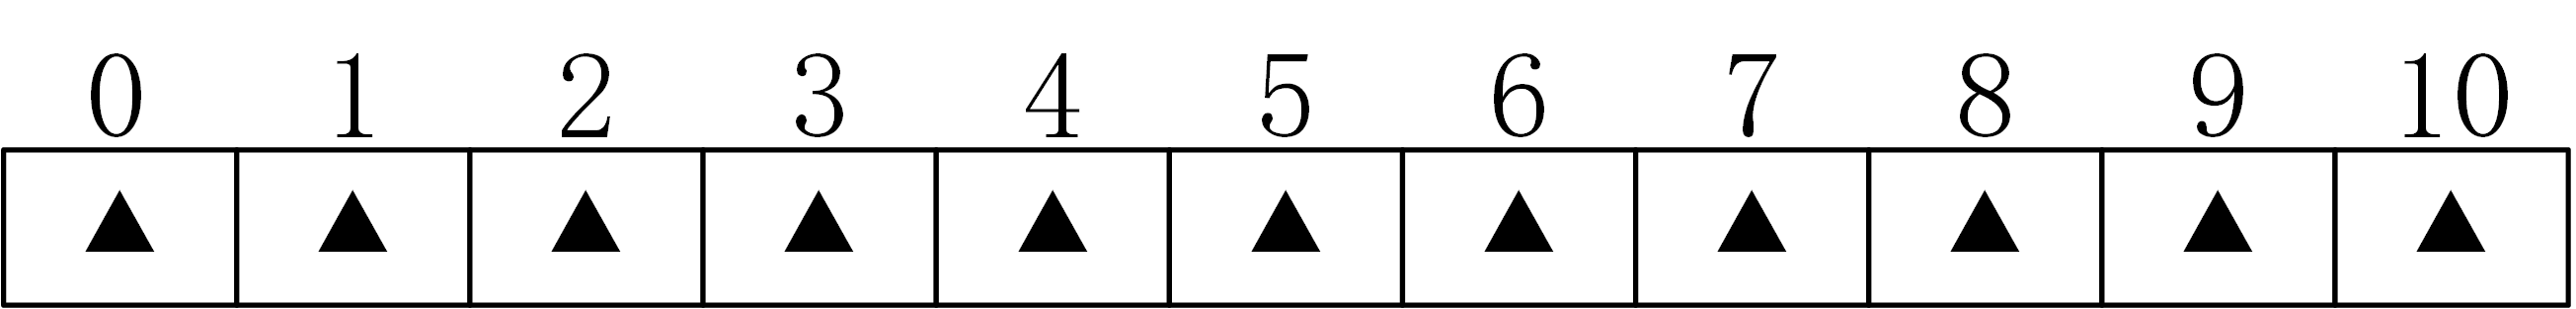
\includegraphics[scale=0.7]{array}}
\only<4->{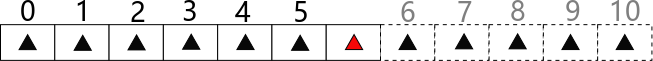
\includegraphics[scale=0.43]{array_2}}
\end{center}

\vspace{6mm}

\uncover<5->{线性链表为\alert{链式结构},在逻辑结构上相邻的元素在物理结构上\alert{不要求}相邻:}
\uncover<6->{\begin{center}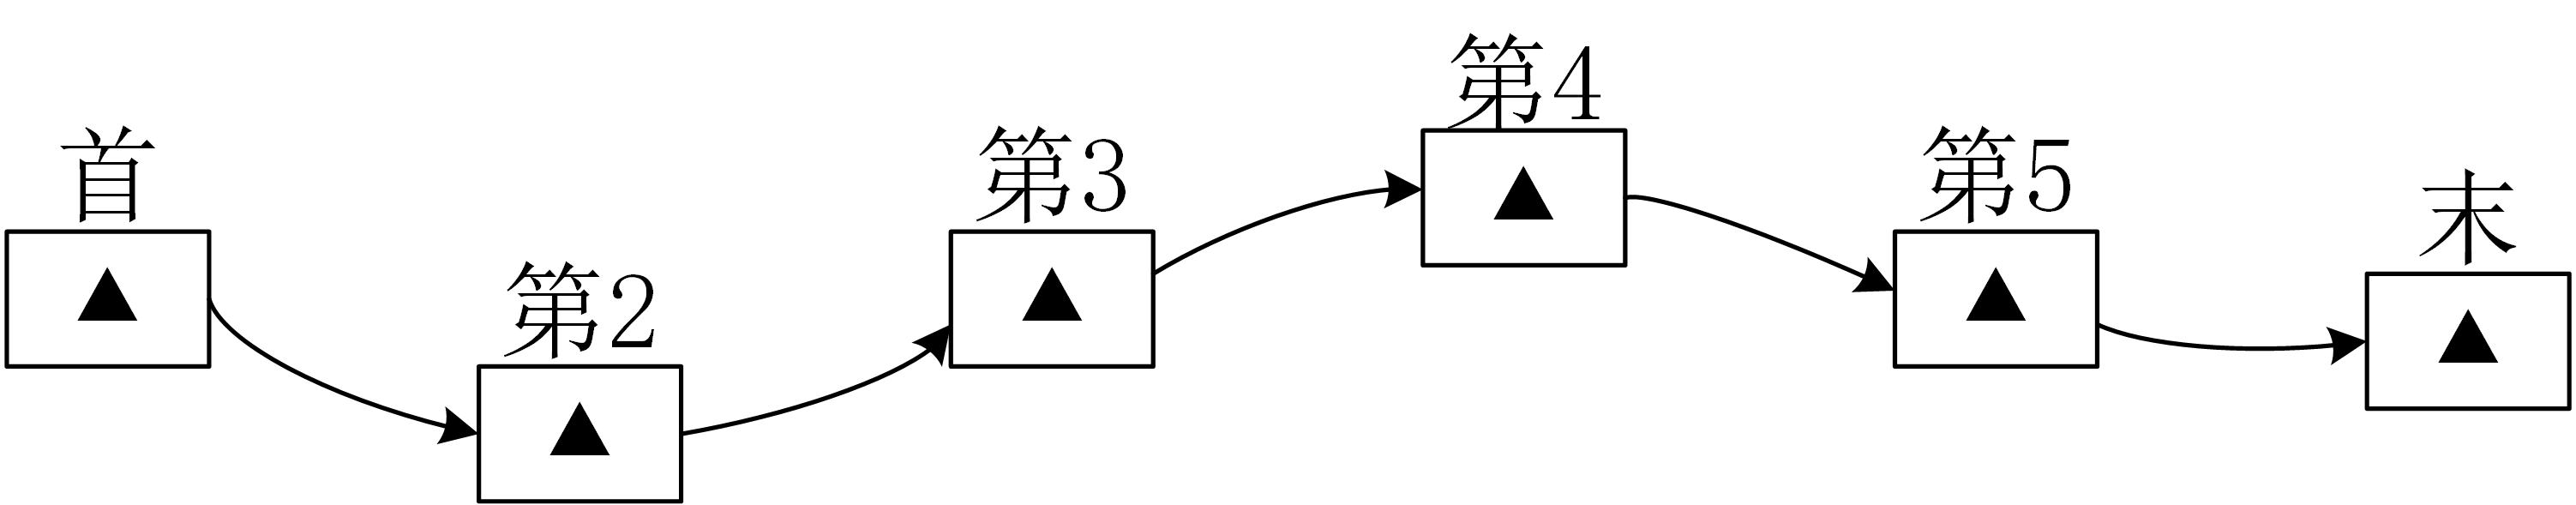
\includegraphics[scale=0.7]{linked_list}\end{center}}

\end{frame}

%-----------------

%++++++++++++++++++++++++++++++++++++++++++++++
\subsection{链表表示}
%++++++++++++++++++++++++++++++++++++++++++++++

%-----------------

\begin{frame}[fragile]{8.3.1~ 链表表示}

每个数据元素占用一个结点,一个结点包含一个\alert{数据域}和一个\alert{指针域},其中指针域存放下一个结点的地址:
\vspace{-1mm}
\begin{center}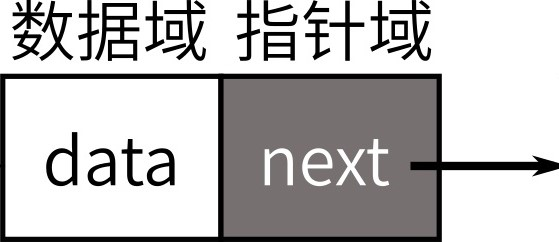
\includegraphics[scale=0.14]{node}\end{center}

\uncover<2->{利用类模板来定义一个结点:}

\vspace{-4mm}

\begin{columns}[t]

\column{0.65\textwidth}
\begin{blueblock}<2->{\texttt{Node}类模板定义}
\begin{lstlisting}[moreemph={Node,T}]
template<typename T>
class Node{
    T m_data; //数据域
    Node *m_next = nullptr; //指向下一个结点的指针
public:
    Node(const T &val) :m_data(val) { }
    const T& data() const{ return m_data; }
    T& data() { return m_data; }
    Node* next() { return m_next; }
};
\end{lstlisting}
\end{blueblock}

\column{0.3\textwidth}
\begin{yellowblock}<2->{说明}
$\bullet$~成员\texttt{m\_next}为指向\texttt{Node}类型的指针。类允许包含指向其自身类型的指针或引用\\
$\bullet$~提供两个版本的\texttt{data}函数以支持\texttt{const}和非\texttt{const}对象的数据访问
\end{yellowblock}

\end{columns}

\end{frame}

%-----------------

\begin{frame}[fragile]{8.3.1~ 链表表示}

单链表的成员包含两个指针,指针head指向表头结点,指针tail指向表尾结点:
\begin{center}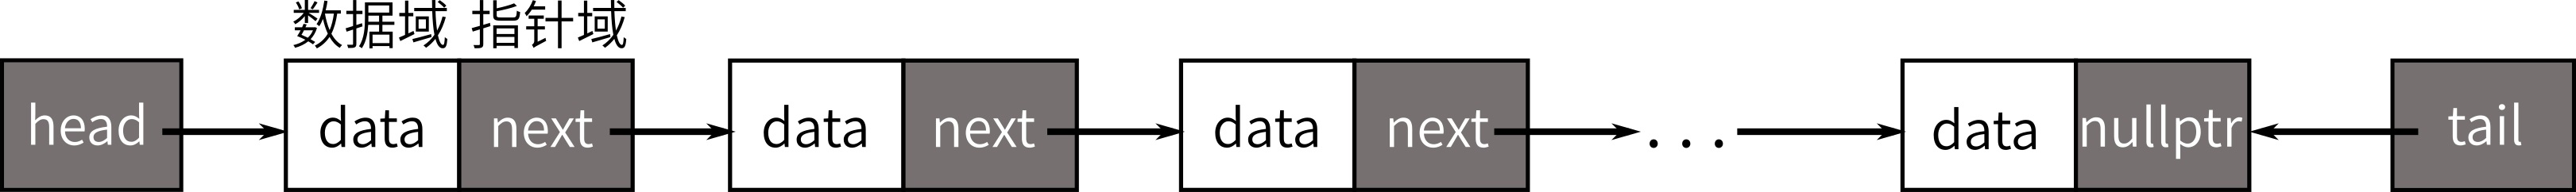
\includegraphics[scale=0.14]{linked_list_2}\end{center}

\vspace{2mm}

\uncover<2->{单链表类模板的定义如下:}

\vspace{-4mm}

\begin{columns}[t]

\column{0.65\textwidth}
\begin{blueblock}<2->{\texttt{SList}类模板定义}
\vspace{-1.5mm}\begin{lstlisting}[moreemph={SList,T,Node}]
template<typename T>
class SList {
    Node<T> *m_head= nullptr, *m_tail= nullptr;
public:
    SList()= default; // 使用默认构造函数
    ~SList();
    void clear();
    void push_back(const T &val);
    Node<T>* insert(Node<T> *pos, const T &val);
    void erase(const T &val);
    Node<T>* find(const T &val);
};
\end{lstlisting}\vspace{-1.5mm}
\end{blueblock}

\column{0.3\textwidth}
\begin{yellowblock}<2->{说明}
$\bullet$~\texttt{clear}函数用来清空链表所有元素\\
$\bullet$~\texttt{push\_back}函数为尾插操作\\
$\bullet$~\texttt{insert}函数在位置\texttt{pos}后插入一个新结点\\
$\bullet$~\texttt{erase}函数删除第一个元素值为\texttt{val}的元素\\
$\bullet$~\texttt{find}函数返回第一个值为\texttt{val}的元素的地址
\end{yellowblock}

\end{columns}

\end{frame}

%-----------------

%++++++++++++++++++++++++++++++++++++++++++++++
\subsection{插入操作}
%++++++++++++++++++++++++++++++++++++++++++++++

%-----------------

\begin{frame}[fragile]{8.3.2~插入操作\normalsize{~---~尾插}}

尾插操作将新结点插入到链表的表尾:
\begin{center}
\only<1>{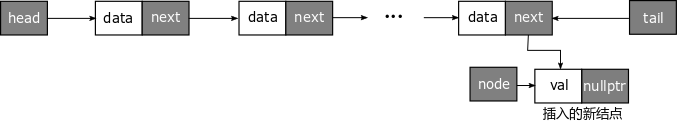
\includegraphics[width=0.85\textwidth]{push_back1}}
\only<2>{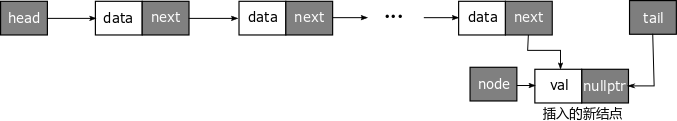
\includegraphics[width=0.85\textwidth]{push_back2}}
\only<3->{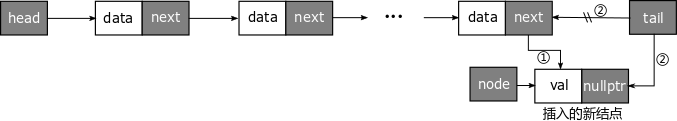
\includegraphics[width=0.85\textwidth]{push_back3}}
\end{center}

\vspace{-6mm}

\uncover<1->{尾插操作定义如下:}

\vspace{-4mm}

\begin{columns}[t]

\column{0.65\textwidth}
\begin{blueblock}<1->{\texttt{push\_back}函数定义}\vspace{-3mm}
\begin{lstlisting}[moreemph={SList,T,Node}]
template<typename T>
void SList<T>::push_back(const T &val) {
     (*@{\alert<1>{Node<T> *node = new Node<T>(val); }}@*)// 创建新结点
    if (m_head == nullptr)
        m_head = m_tail= node;
    else {
        (*@{\alert<1>{ m\_tail->m\_next = node;}}@*)
         (*@{\alert<2>{m\_tail = node;}}@*)
    }
}
\end{lstlisting}\vspace{-3mm}
\end{blueblock}

\column{0.3\textwidth}
\begin{yellowblock}<2->{说明}
$\bullet$~使用形参的数据创建新结点\\
$\bullet$~如果为空,将创建的结点作为头结点(也是尾结点)\\
$\bullet$~否则,将尾结点指向该结点,并将尾指针后移,使其指向新的尾结点
\end{yellowblock}

\end{columns}

\end{frame}

%-----------------

\begin{frame}[fragile]{8.3.2~插入操作\normalsize{~---~指定位置插入}}

插入操作将新结点插入到链表的指定位置:
%\begin{center}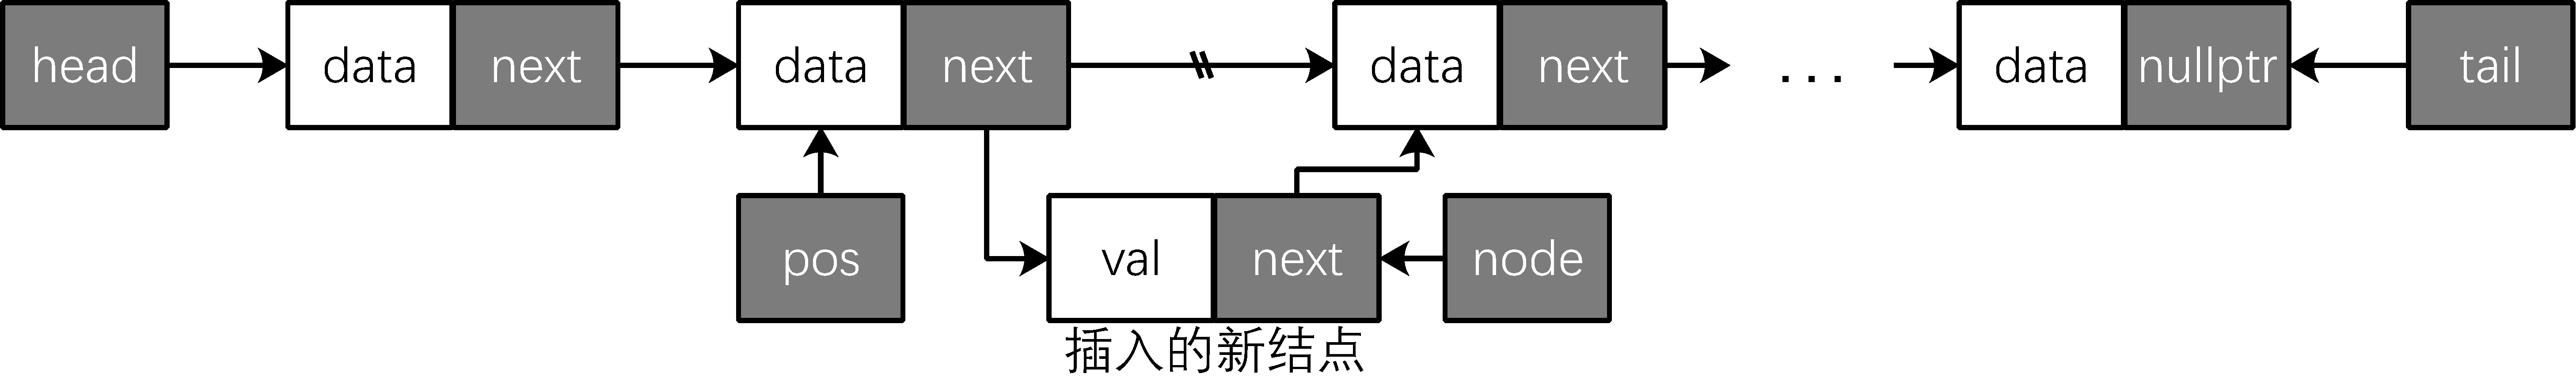
\includegraphics[width=\textwidth]{insert}\end{center}
\begin{center}
\only<1>{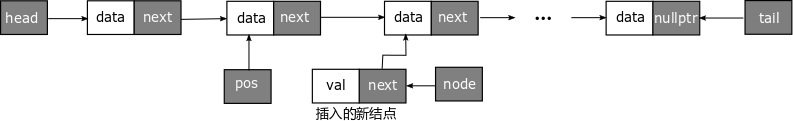
\includegraphics[width=0.85\textwidth]{insert1}}
\only<2>{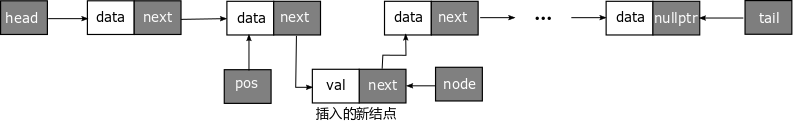
\includegraphics[width=0.85\textwidth]{insert2}}
\only<3->{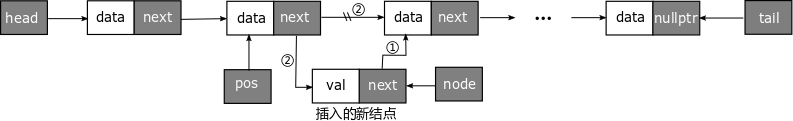
\includegraphics[width=0.85\textwidth]{insert3}}
\end{center}
\vspace{-4mm}

\uncover<1->{插入操作定义如下:}

\vspace{-4mm}

\begin{columns}[t]

\column{0.6\textwidth}
\begin{blueblock}<1->{\texttt{insert}函数定义}
\begin{lstlisting}[moreemph={SList,T,Node}]
template<typename T>
Node<T>* SList<T>::insert(Node<T> *pos, const T &val) {
    (*@{\alert<1>{Node<T> *node = new Node<T>(val);}}@*) // 创建新结点
    (*@{\alert<1>{node->m\_next = pos->m\_next;}}@*)
   (*@{\alert<2>{ pos->m\_next = node;}}@*)
    if (pos == m_tail) // 判断pos是否为尾结点
        m_tail = node;
    return node;
}
\end{lstlisting}
\end{blueblock}

\column{0.35\textwidth}
\begin{yellowblock}<2->{说明}
$\bullet$~将新结点的指针域指向\texttt{pos}的后继,再将\texttt{pos}的后继修改为\texttt{node}\\
$\bullet$~如果\texttt{pos}为尾结点,需要修改尾指针指向新结点
\end{yellowblock}
\vspace{-2mm}
\begin{redblock}<3->{注意}
\texttt{pos}必须为非空链表的某一个结点指针
\end{redblock}

\end{columns}

\end{frame}

%-----------------

\begin{frame}[fragile]{8.3.2~插入操作\normalsize{~---~指定位置插入}}

利用成员函数\texttt{find}找到要插入的位置,\texttt{find}的实现如下:

\vspace{-4mm}

\begin{columns}[t]

\column{0.65\textwidth}
\begin{blueblock}{\texttt{insert}函数定义}
\begin{lstlisting}[moreemph={SList,T,Node}]
template<typename T>
Node<T>* SList<T>::find(const T &val) {
    Node<T> *p = m_head;
    while (p != nullptr && p->m_data != val)
        p = p->m_next;
    return p;
}
\end{lstlisting}
\end{blueblock}

\column{0.3\textwidth}
\begin{yellowblock}{说明}
$\bullet$~从表头开始扫描,逐个元素进行匹配\\
$\bullet$~如果找到则返回此元素的地址\\
$\bullet$~否则返回一个空指针
\end{yellowblock}

\end{columns}

\end{frame}

%-----------------

%++++++++++++++++++++++++++++++++++++++++++++++
\subsection{删除操作}
%++++++++++++++++++++++++++++++++++++++++++++++

%-----------------

\begin{frame}[fragile]{8.3.3~删除操作}

成员函数\texttt{erase}根据指定的内容,删除在链表中第一次出现的元素:
\begin{center}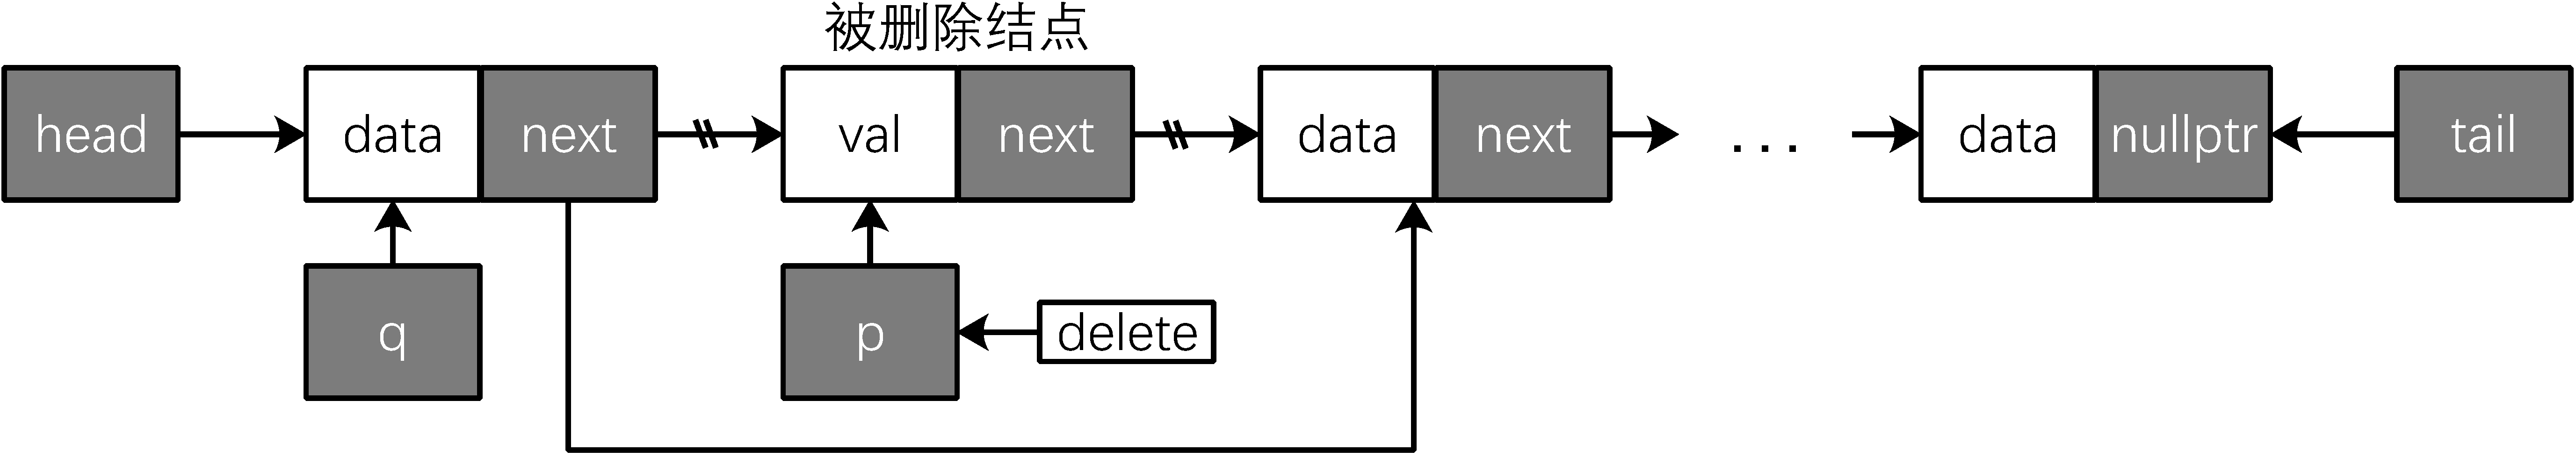
\includegraphics[width=\textwidth]{erase}\end{center}

\vspace{-6mm}

\begin{columns}[t]

\column{0.65\textwidth}
\begin{blueblock}<2->{\texttt{erase}函数定义}
\vspace{-2mm}\begin{lstlisting}[moreemph={SList,T,Node}]
template<typename T> void SList<T>::erase(const T &val) {
    Node<T> *p = m_head, *q = p;
    while (p != nullptr && p->m_data != val) {
        q = p;         p = p->m_next;
    }
    if (p) q->m_next = p->m_next;
    if (p == m_tail) m_tail = q;
    if (p == m_head) m_head = nullptr;
    delete p;
}
\end{lstlisting}\vspace{-2mm}
\end{blueblock}

\column{0.3\textwidth}
\begin{yellowblock}<2->{说明}
$\bullet$~如果找到,即指针\texttt{p}非空,将其从链表中移除\\
$\bullet$~如果\texttt{p}为表尾元素,修改\texttt{tail}指针\\
$\bullet$~如果\texttt{p}为表头元素,修改\texttt{head}指针为空指针
\end{yellowblock}

\end{columns}

\end{frame}

%-----------------

%++++++++++++++++++++++++++++++++++++++++++++++
\subsection{清空链表}
%++++++++++++++++++++++++++++++++++++++++++++++

%-----------------

\begin{frame}[fragile]{8.3.4~清空链表}

成员函数\texttt{clear}实现从表头开始,逐个移除链表中每个结点并释放其内存

\vspace{-4mm}

\begin{columns}[t]

\column{0.65\textwidth}
\begin{blueblock}{\texttt{clear}函数定义}
\vspace{-2mm}\begin{lstlisting}[moreemph={SList,T,Node}]
template<typename T>
void SList<T>::clear() {
    Node<T> *p = nullptr;
    while (m_head != nullptr) {
        p = m_head;                 //p 指向当前表头结点
        m_head = m_head->m_next;    //表头结点后移
        delete p;                   //释放 p 所指向的内存
    }
    m_tail = nullptr;               //将尾指针 tail 置空
}
\end{lstlisting}\vspace{-2mm}
\end{blueblock}

\column{0.3\textwidth}

\end{columns}

\vspace{2mm}

\uncover<2->{在析构函数里面,可以直接调用clear函数释放链表的内存空间:}

\vspace{-4mm}

\begin{columns}[t]

\column{0.65\textwidth}
\begin{blueblock}<2->{\texttt{SList}析构函数定义}
\vspace{-2mm}\begin{lstlisting}[moreemph={SList,T,Node}]
template<typename T>
SList<T>::~SList() {    clear(); }
\end{lstlisting}\vspace{-3mm}
\end{blueblock}

\column{0.3\textwidth}

\end{columns}

\end{frame}

%-----------------

%++++++++++++++++++++++++++++++++++++++++++++++
\subsection{打印链表}
%++++++++++++++++++++++++++++++++++++++++++++++

%-----------------

\begin{frame}[fragile]{8.3.5~打印链表}

为了像内置类型一样输出,需要重载输出运算符,并将其声明为\texttt{SList}的友元:

\vspace{-4mm}

\begin{columns}[t]

\column{0.71\textwidth}
\begin{blueblock}{重载输出运算符声明及友元声明}
\vspace{-2.5mm}\begin{lstlisting}[moreemph={T,SList,Node}]
template<typename T> ostream& operator<<(ostream&,const SList<T>&);
template<typename T>
class SList {
    friend ostream& operator<< (*@{\alert{<T>}}@*)(ostream&,const SList<T>&);
    //其它成员定义保持不变
};
\end{lstlisting}\vspace{-2.5mm}
\end{blueblock}
\vspace{-2mm}
\begin{blueblock}{重载输出运算符定义}
\vspace{-2.5mm}\begin{lstlisting}[moreemph={T,SList,Node}]
template<typename T>
ostream& operator<<(ostream &os, const SList<T>& list) {
    Node<T> *p = list.m_head;
    while (p != nullptr) {
        os << p->data() << " "; // 类型T支持<<运算符
        p = p->next();
    }
    return os;
}
\end{lstlisting}\vspace{-2.5mm}
\end{blueblock}

\column{0.24\textwidth}
\begin{redblock}<2->{注意}
友元关系被限定在相同类型实例化的输出运算符和\texttt{SList}之间
\end{redblock}

\end{columns}

\end{frame}

%-----------------

%++++++++++++++++++++++++++++++++++++++++++++++
\subsection{拷贝控制与友元声明}
%++++++++++++++++++++++++++++++++++++++++++++++

%-----------------

\begin{frame}[fragile]{8.3.6~拷贝控制与友元声明}

回顾类模板 Node的定义,如果使用默认的复制与赋值操作会有什么问题?

\vspace{-4mm}

\begin{columns}[t]

\column{0.65\textwidth}
\begin{blueblock}{\texttt{Node}类模板部分定义}\vspace{-3mm}
\begin{lstlisting}[moreemph={Node,T}]
template<typename T>
class Node{
    T m_data; //数据域
    Node *m_next = nullptr; //指针域
    /*...*/
};
\end{lstlisting}\vspace{-3mm}
\end{blueblock}

\column{0.3\textwidth}
\begin{greenblock}<2->{答案}
根据链表中的一个结点创建一个新结点(或赋值操作)时,会导致两个结点的指针域指向链表中的同一个结点
\end{greenblock}

\end{columns}

\vspace{2mm}

\uncover<3->{应该利用~\alert{\texttt{delete}关键字}禁止\texttt{Node}类型实例的复制与赋值:}

\vspace{-4mm}

\begin{columns}[t]

\column{0.65\textwidth}
\begin{blueblock}<3->{\texttt{Node}类模板部分定义}\vspace{-3mm}
\begin{lstlisting}[moreemph={SList,Node,T}]
template<typename T>
class Node {
public:
    Node(const Node &rhs) = delete;
    Node& operator =(const Node &rhs) = delete;
    // 其它成员定义保持不变
};
\end{lstlisting}\vspace{-2.5mm}
\end{blueblock}

\column{0.3\textwidth}

\end{columns}

\end{frame}

%-----------------

\begin{frame}[fragile]{8.3.6~拷贝控制与友元声明}

类似的,也不允许\texttt{SList}类型实例的复制与赋值:

\vspace{-4mm}

\begin{columns}[t]

\column{0.65\textwidth}
\begin{blueblock}{\texttt{SList}类模板部分定义}
\vspace{-2.5mm}\begin{lstlisting}[moreemph={SList,Node,T}]
template<typename T>
class SList {
public:
    SList(const SList &) = delete;
    SList& operator=(const SList &) = delete;
    //其它成员定义保持不变
};
\end{lstlisting}\vspace{-2.5mm}
\end{blueblock}

\column{0.3\textwidth}

\end{columns}

\vspace{2mm}

\uncover<2->{此外,还需要将类模板\texttt{SList}声明为\texttt{Node}的友元,否则有什么问题?}

\vspace{-4mm}

\begin{columns}[t]

\column{0.65\textwidth}
\begin{blueblock}<2->{\texttt{Node}类模板部分定义}
\vspace{-2.5mm}\begin{lstlisting}[moreemph={SList,Node,T}]
template<typename T> class SList; //前向声明
template<typename T>
class Node {
    friend class SList<T>; // 将SList声明为Node的友元
    // 其它成员定义保持不变
};
\end{lstlisting}\vspace{-2.5mm}
\end{blueblock}

\column{0.3\textwidth}
\begin{greenblock}<3->{答案}
在\texttt{SList}的成员函数中将没有权限直接使用\texttt{m\_next}
\end{greenblock}

\end{columns}

\end{frame}

%-----------------

\begin{frame}[fragile]{8.3.6~拷贝控制与友元声明}

创建一个存放整型元素的单链表对尾插、指定位置插入、删除等操作进行测试:

\vspace{-4mm}

\begin{columns}[t]

\column{0.65\textwidth}
\begin{blueblock}{使用\texttt{SList}类模板}
\begin{lstlisting}[moreemph={SList,Node,T}]
SList<int> l;
int val;
while (cin >> val) { // 输入10 20 30三个数据
    l.push_back(val);
}
cout << l << endl;
Node<int> *pos = l.find(20);
l.insert(pos, 25);
cout << l << endl;
l.erase(25);
cout << l << endl;
\end{lstlisting}
\end{blueblock}

\column{0.3\textwidth}
\begin{greenblock}{问题}
输出结果是什么?
\end{greenblock}
\begin{greenblock}<2->{答案}
输出结果为:\\
\texttt{10 20 30}\\
\texttt{10 20 25 30}\\
\texttt{10 20 30}
\end{greenblock}

\end{columns}

\end{frame}

%-----------------

%##################################################################
\section{链栈}
%##################################################################

%-----------------

\begin{frame}[fragile]{8.4~链栈}

\begin{block}{链栈}
栈是一种\alert{只能在一端}进行插入和删除操作的线性表。栈也称为\alert{后进先出}线性表。\\
~\\
允许进行插入和删除操作的一端称为栈顶,另一端称为栈底。
\end{block}

\begin{center}
  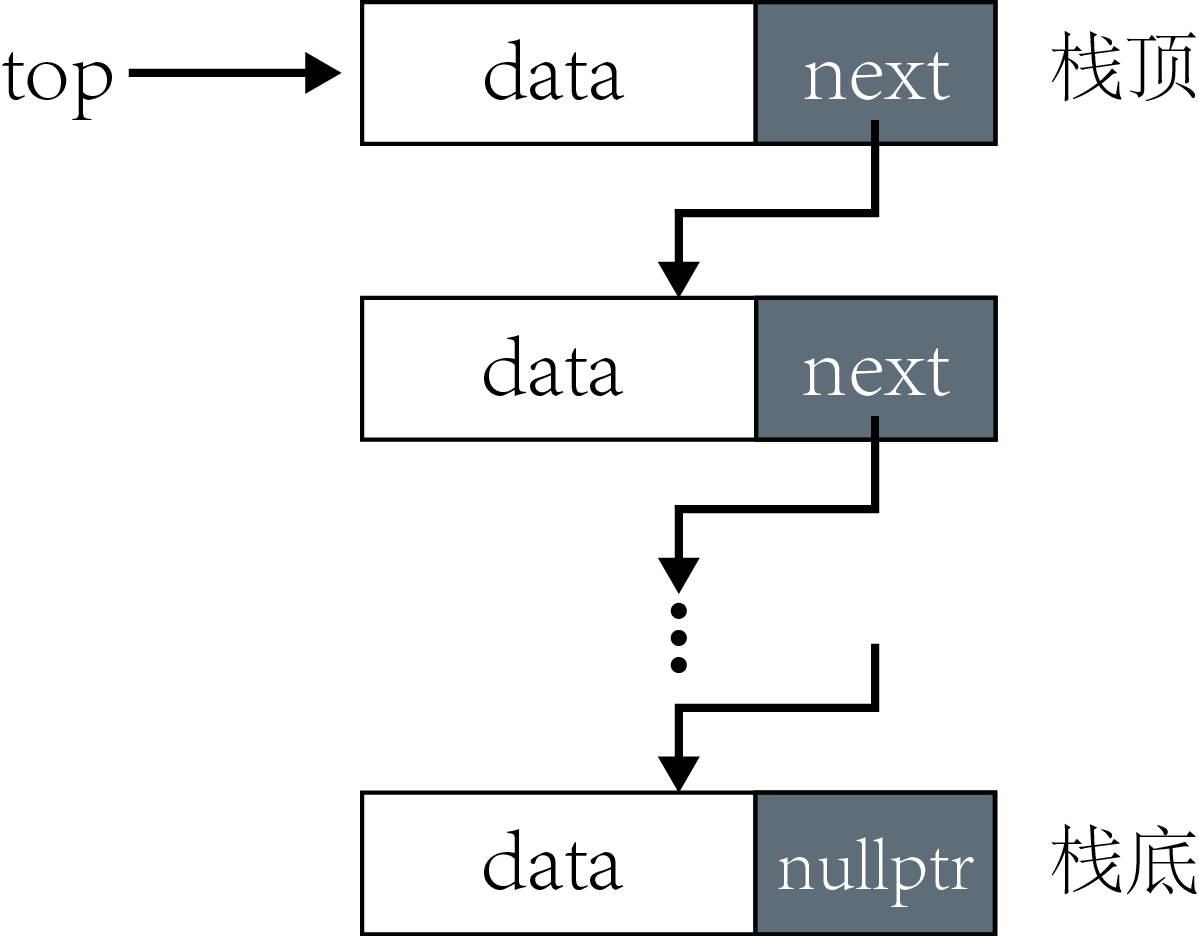
\includegraphics[height=0.4\textheight]{stack}
\end{center}

\end{frame}

%-----------------

%++++++++++++++++++++++++++++++++++++++++++++++
\subsection{链栈表示与操作}
%++++++++++++++++++++++++++++++++++++++++++++++

%-----------------

\begin{frame}[fragile]{8.4.1~链栈表示与操作}

链栈支持进栈、出栈、清空、取栈顶元素和判断是否为空等操作。\\
模板类\texttt{Stack}定义如下:

\vspace{-4mm}

\begin{columns}[t]

\column{0.65\textwidth}
\begin{blueblock}{\texttt{Stack}类模板定义}
\begin{lstlisting}[moreemph={Node,T,Stack}]
template<typename T>
class Stack {
    Node<T> *m_top = nullptr;
public:
    Stack() = default; //使用默认构造函数
    Stack(const Stack &) = delete;
    Stack& operator=(const Stack &) = delete;
    ~Stack();
    void clear();
    void push(const T &val);
    void pop();
    bool empty() const { return m_top == nullptr; }
    const T& top() { return m_top->m_data; }
};
\end{lstlisting}
\end{blueblock}

\column{0.3\textwidth}
\begin{yellowblock}{说明}
$\bullet$~类似\texttt{SList},\texttt{Stack}类模板禁止复制和赋值操作\\
$\bullet$~\texttt{clear}函数执行清空栈操作\\
$\bullet$~\texttt{push}函数执行进栈操作\\
$\bullet$~\texttt{pop}函数执行出栈操作\\
$\bullet$~\texttt{empty}函数判断栈是否为空\\
$\bullet$~\texttt{top}函数取栈顶元素。 返回栈顶元素的\texttt{const}引用,意味着只能对栈顶元素进行读
操作,\alert{不能执行写操作}
\end{yellowblock}

\end{columns}

\end{frame}

%-----------------

\begin{frame}[fragile]{8.4.1~链栈表示与操作\normalsize{~---~进栈与出栈操作}}

进栈操作的实现如下:

\vspace{-4mm}

\begin{columns}[t]

\column{0.65\textwidth}
\begin{blueblock}{\texttt{push}函数定义}
\vspace{-2mm}\begin{lstlisting}[moreemph={Node,T,Stack}]
template<typename T>
void Stack<T>::push(const T &val) {
    Node<T> *node = new Node<T>(val);
    node->m_next = m_top;
    m_top = node;
}
\end{lstlisting}\vspace{-2mm}
\end{blueblock}

\column{0.3\textwidth}
\begin{yellowblock}{说明}
创建一个新结点 \texttt{node},然后将结点\texttt{node}压栈,最后修改栈顶指针,使其指向新的栈顶结点
\end{yellowblock}

\end{columns}

\vspace{2mm}

\uncover<2->{出栈操作的实现如下:}

\vspace{-4mm}

\begin{columns}[t]

\column{0.65\textwidth}
\begin{blueblock}<2->{\texttt{pop}函数定义}
\vspace{-2mm}\begin{lstlisting}[moreemph={Node,T,Stack}]
template<typename T>
void Stack<T>::pop() {
    if (empty()) return;
    Node<T> *p = m_top;
    m_top = m_top->m_next;
    delete p;
}
\end{lstlisting}\vspace{-2mm}
\end{blueblock}

\column{0.3\textwidth}
\begin{yellowblock}<2->{说明}
先把栈顶元素地址保存起来,然后修改栈顶指针,使其指向新的栈顶元素,最后通过保存的指针释放原来栈顶元素的内存
\end{yellowblock}

\end{columns}

\end{frame}

%-----------------

\begin{frame}[fragile]{8.4.1~链栈表示与操作\normalsize{~---~清空操作}}

清空操作的实现如下:

\vspace{-4mm}

\begin{columns}[t]

\column{0.65\textwidth}
\begin{blueblock}{\texttt{push}函数定义}
\vspace{-2mm}\begin{lstlisting}[moreemph={Node,T,Stack}]
template<typename T>
void Stack<T>::clear() {
    Node<T> *p = nullptr;
    while (m_top != nullptr) {
        p = m_top;
        m_top = m_top->m_next;
        delete p;
    }
}
\end{lstlisting}\vspace{-2mm}
\end{blueblock}

\column{0.3\textwidth}
\begin{yellowblock}{说明}
利用出栈的操作,逐个释放每个元素的内存空间
\end{yellowblock}

\end{columns}

\vspace{2mm}

\uncover<2->{在析构函数中调用\texttt{clear}函数释放所有结点的内存:}

\vspace{-4mm}

\begin{columns}[t]

\column{0.65\textwidth}
\begin{blueblock}<2->{\texttt{Stack}析构函数定义}
\vspace{-2mm}\begin{lstlisting}[moreemph={Node,T,Stack}]
template<typename T>
Stack<T>::~Stack() {
    clear();
}
\end{lstlisting}\vspace{-2mm}
\end{blueblock}

\column{0.3\textwidth}

\end{columns}

\end{frame}

%-----------------

%++++++++++++++++++++++++++++++++++++++++++++++
\subsection{简单计算器}
%++++++++++++++++++++++++++++++++++++++++++++++

%-----------------

\begin{frame}[fragile]{8.4.2~简单计算器}

\alert{表达式求值}是栈的重要应用之一, 假设有如下算术表达式:\\
\begin{center}{\Large \texttt{\alert<3>{a} \alert<4>{-} \alert<5>{b} \alert<6>{/} \alert<7>{c} \alert<8-13>{+} \alert<14>{d} \alert<15>{*} \alert<16>{e} \alert<17->{=}}}\end{center}

\only<2>{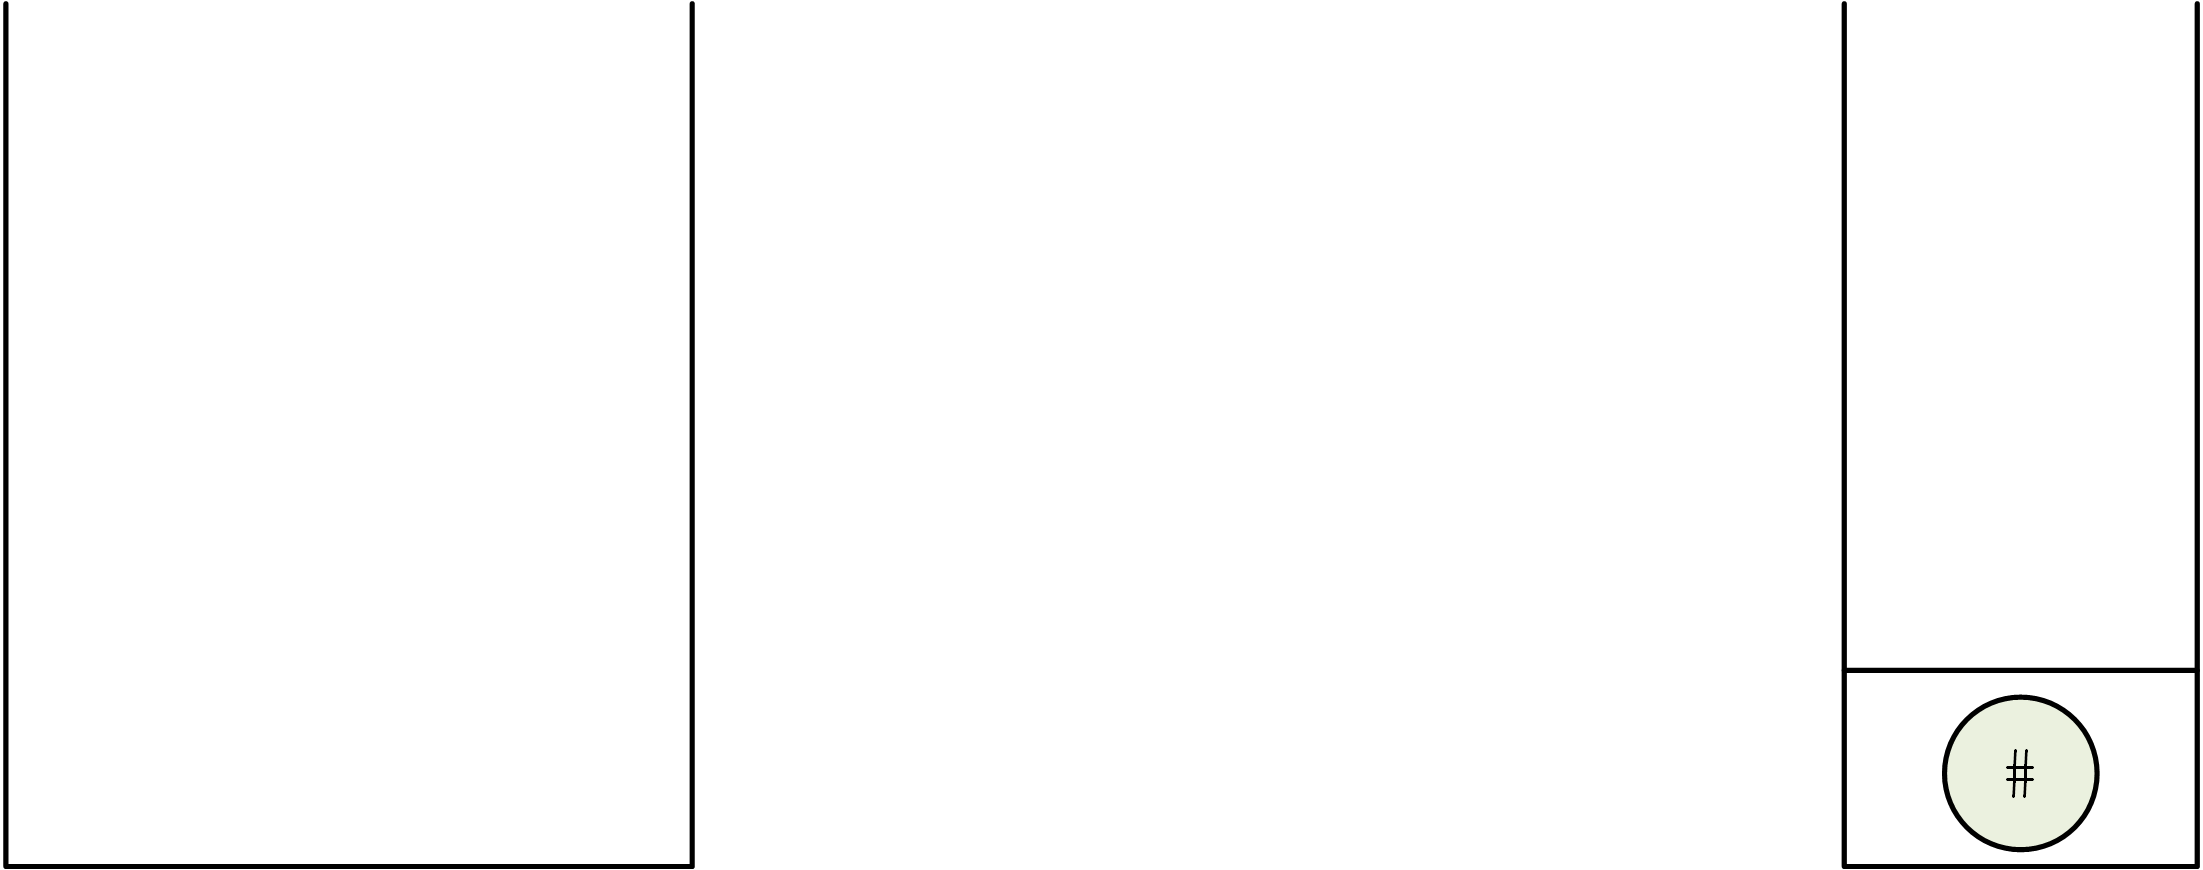
\includegraphics[width=\textwidth]{calculate_1}}
\only<3>{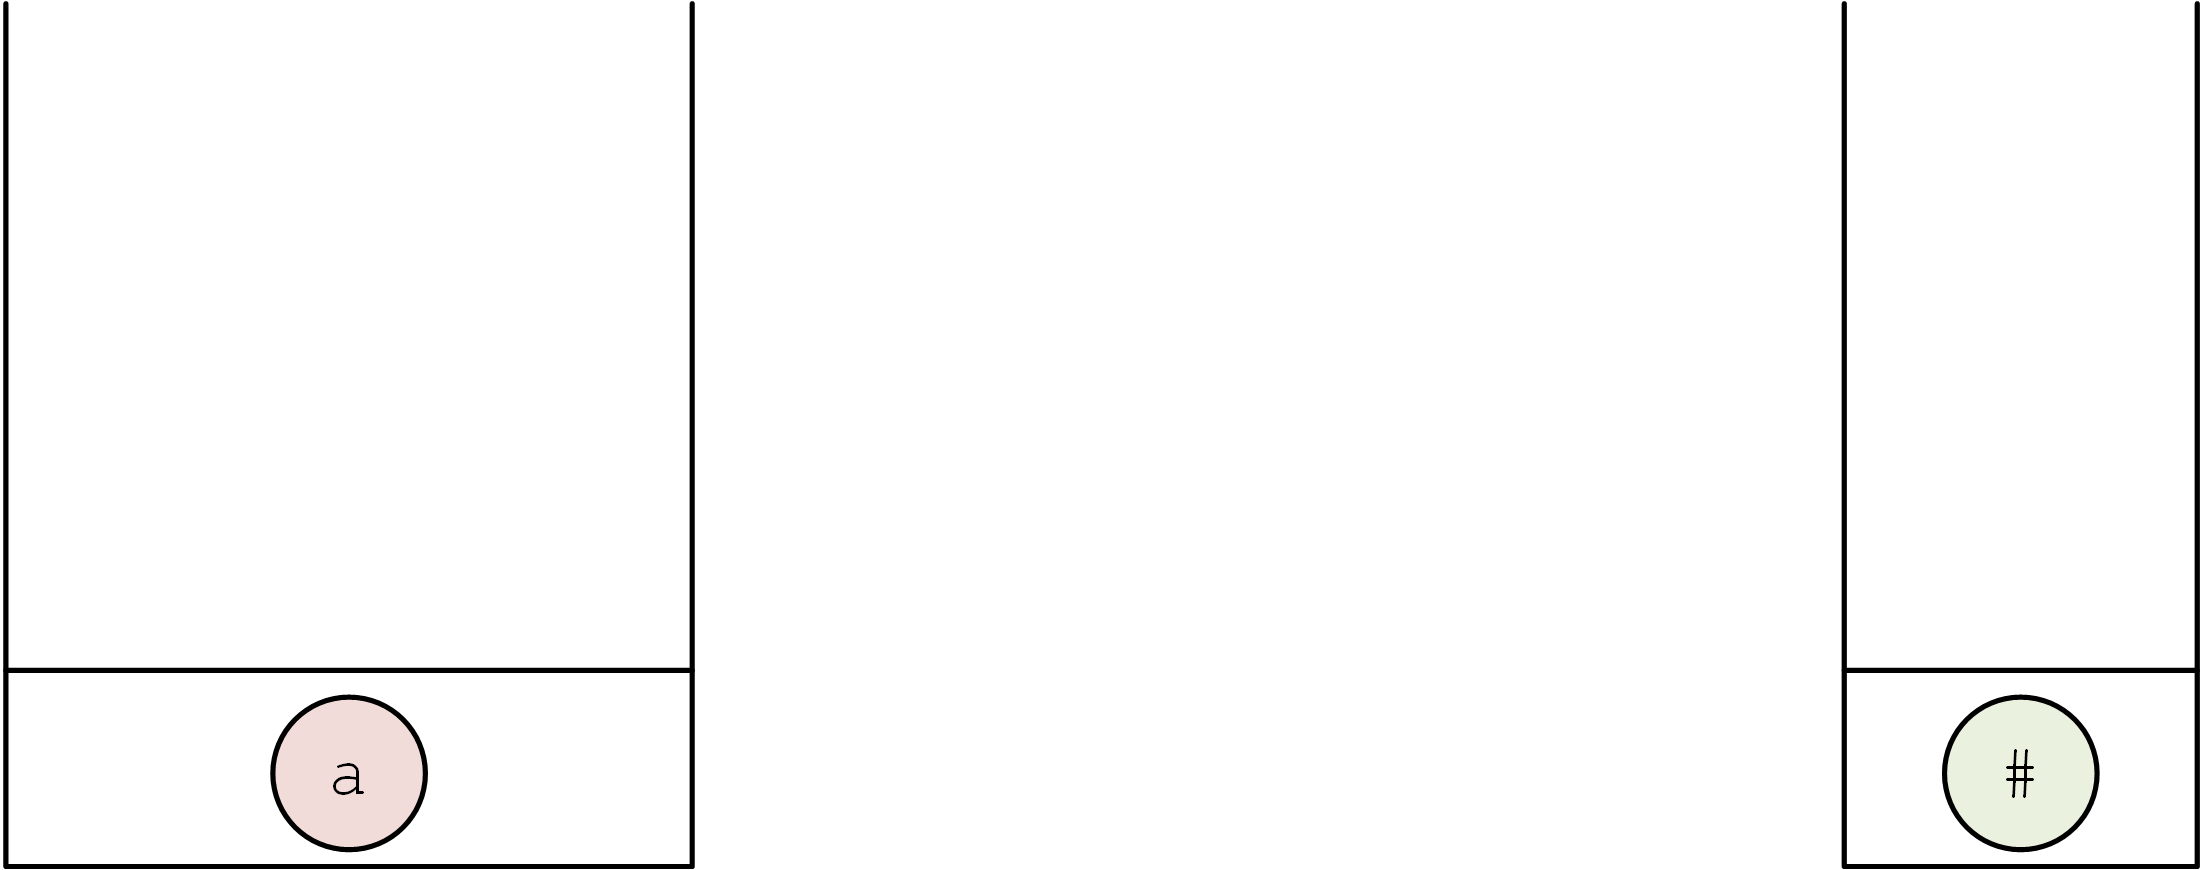
\includegraphics[width=\textwidth]{calculate_2}}
\only<4>{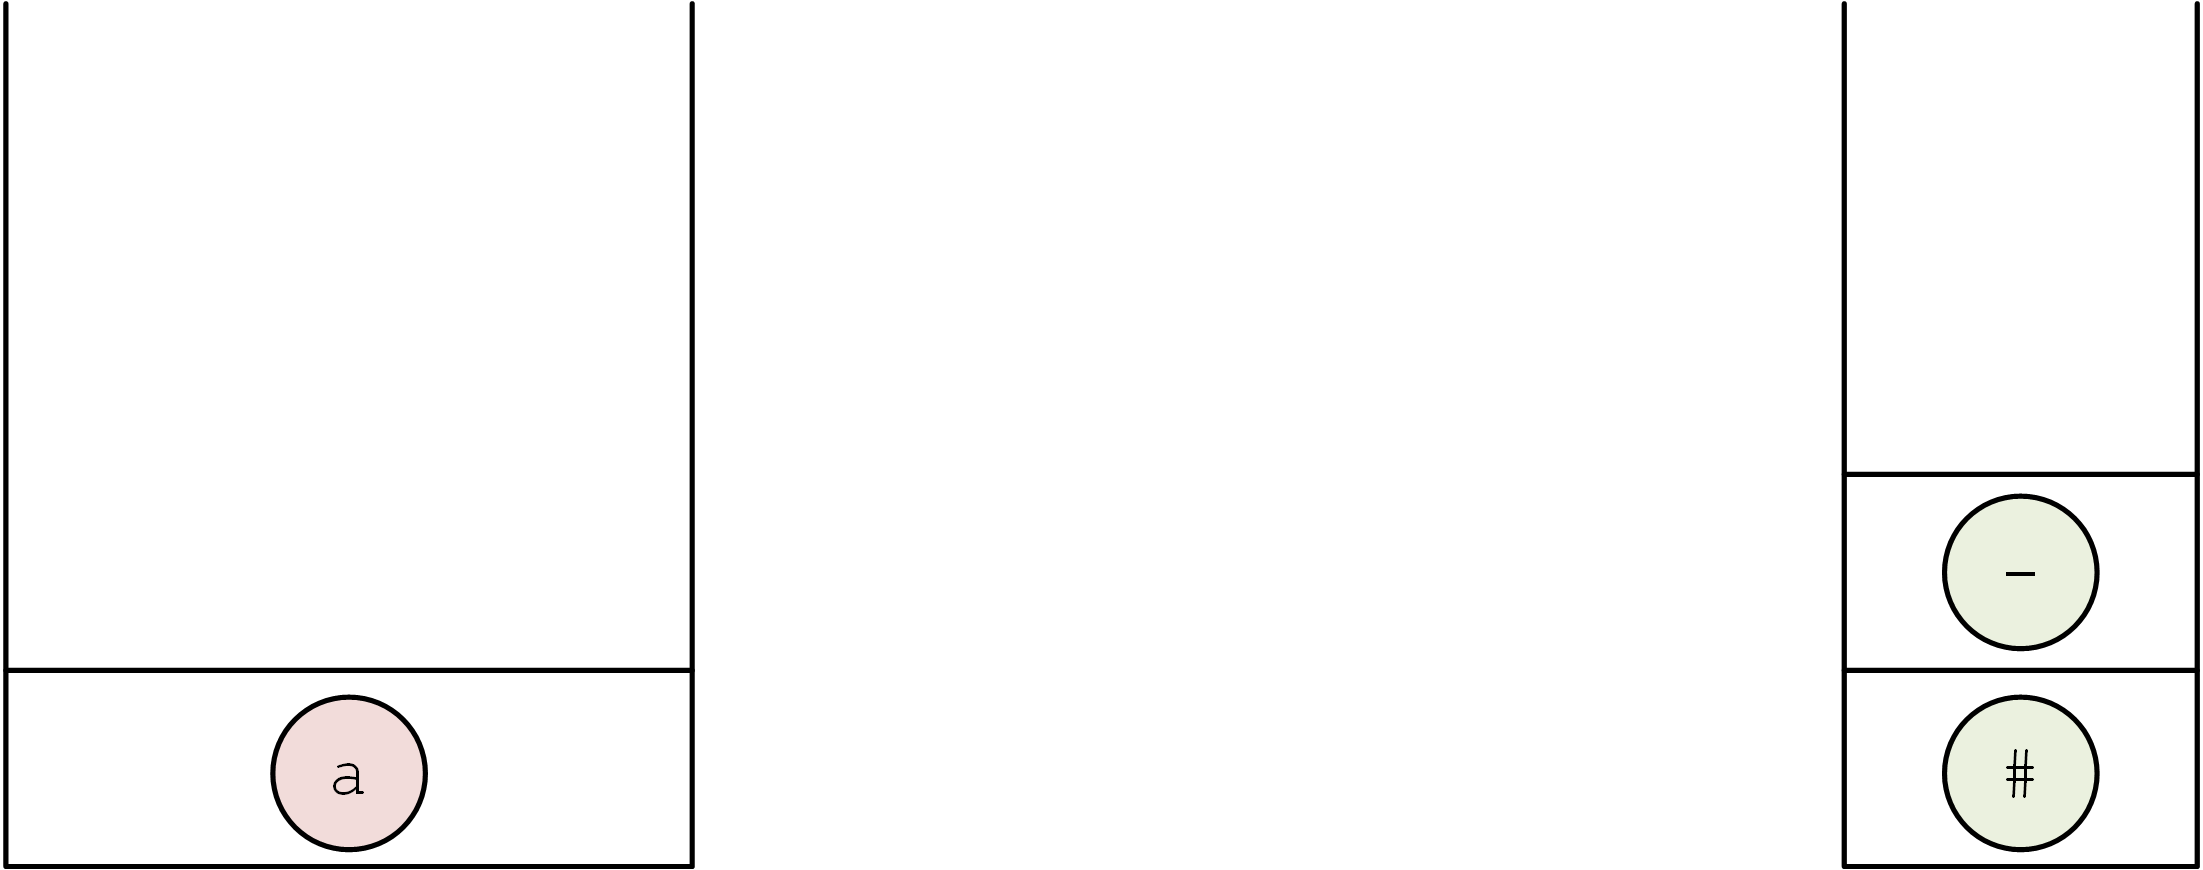
\includegraphics[width=\textwidth]{calculate_3}}
\only<5>{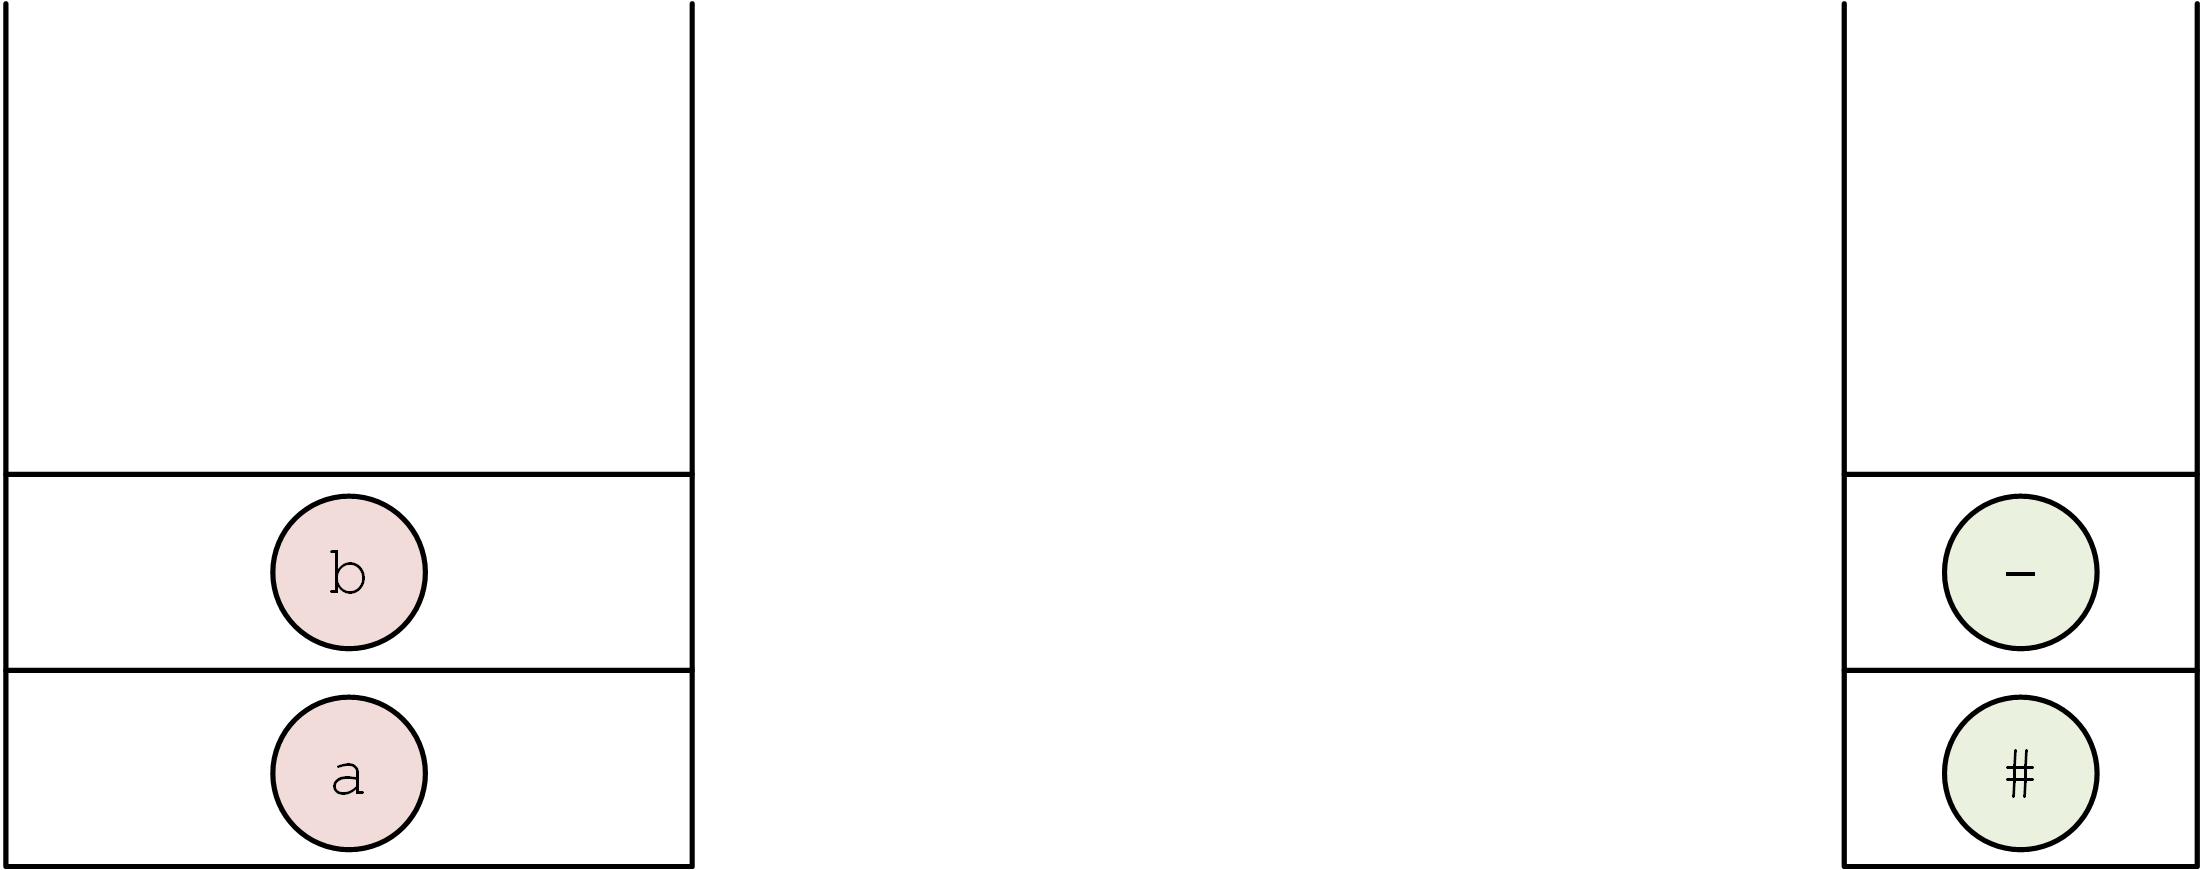
\includegraphics[width=\textwidth]{calculate_4}}
\only<6>{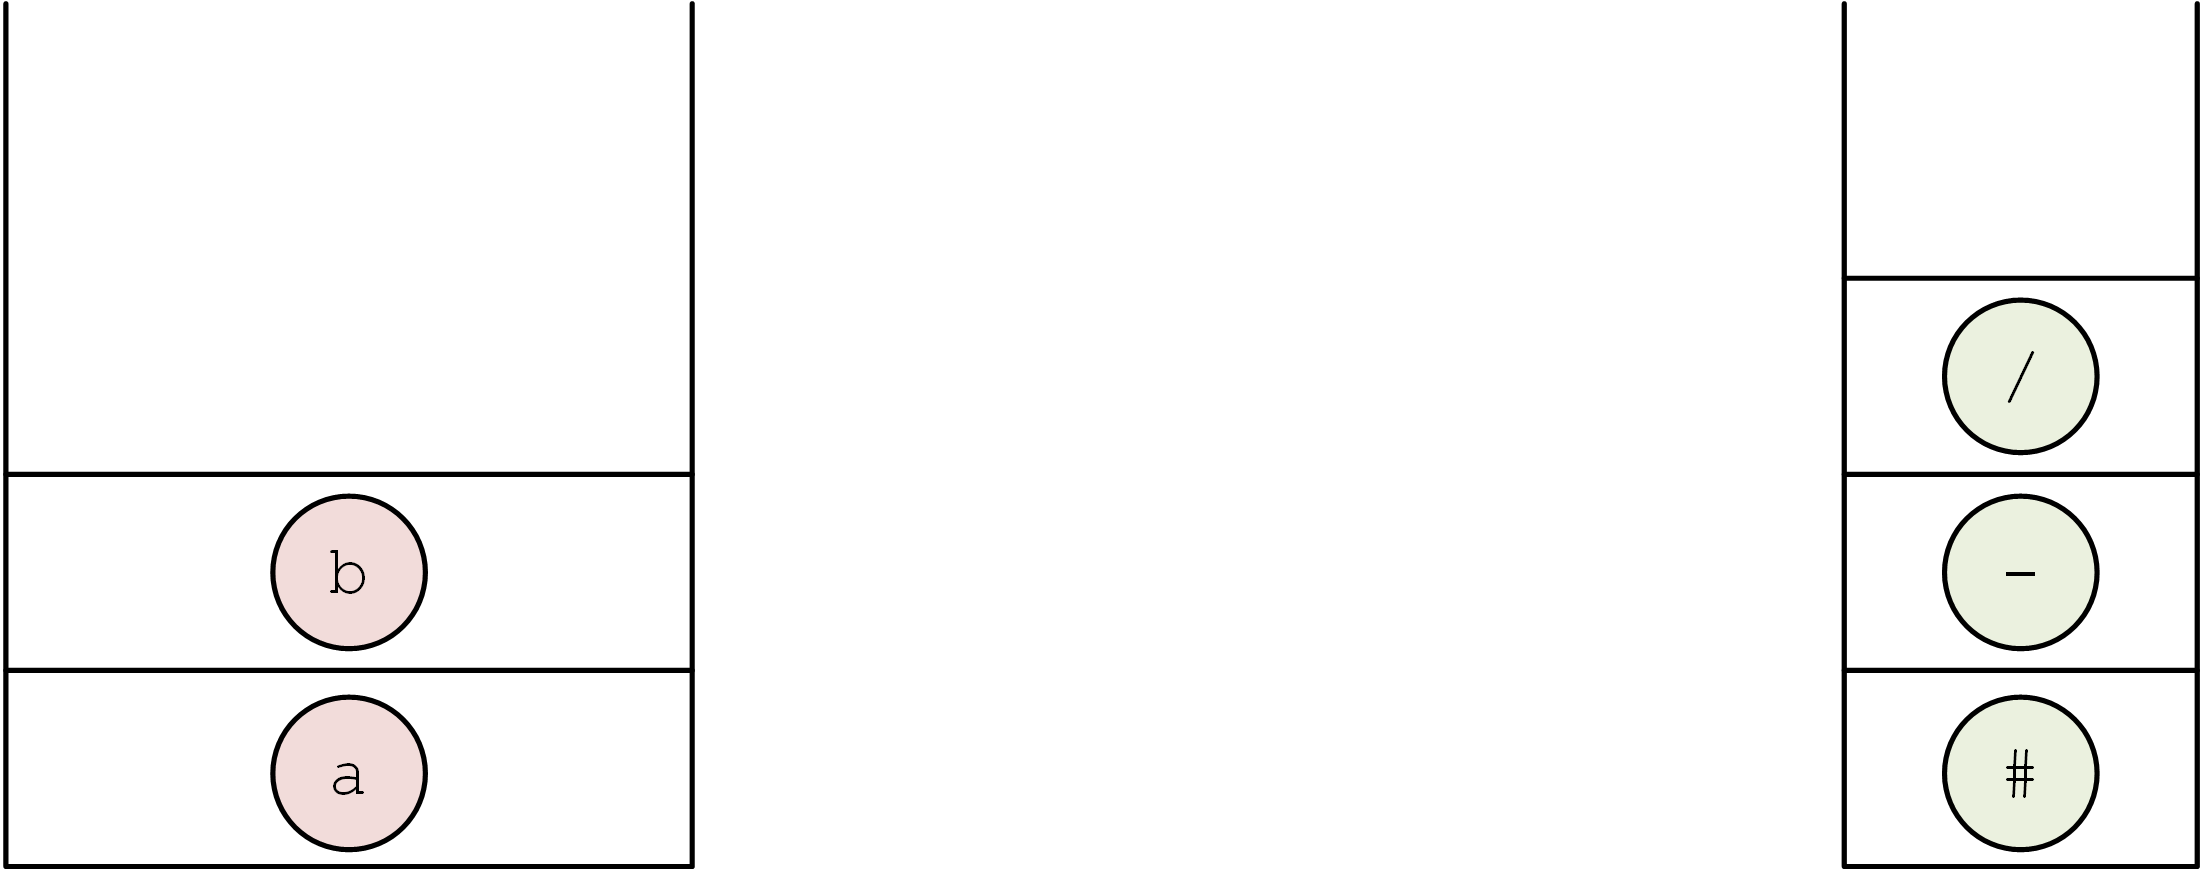
\includegraphics[width=\textwidth]{calculate_5}}
\only<7>{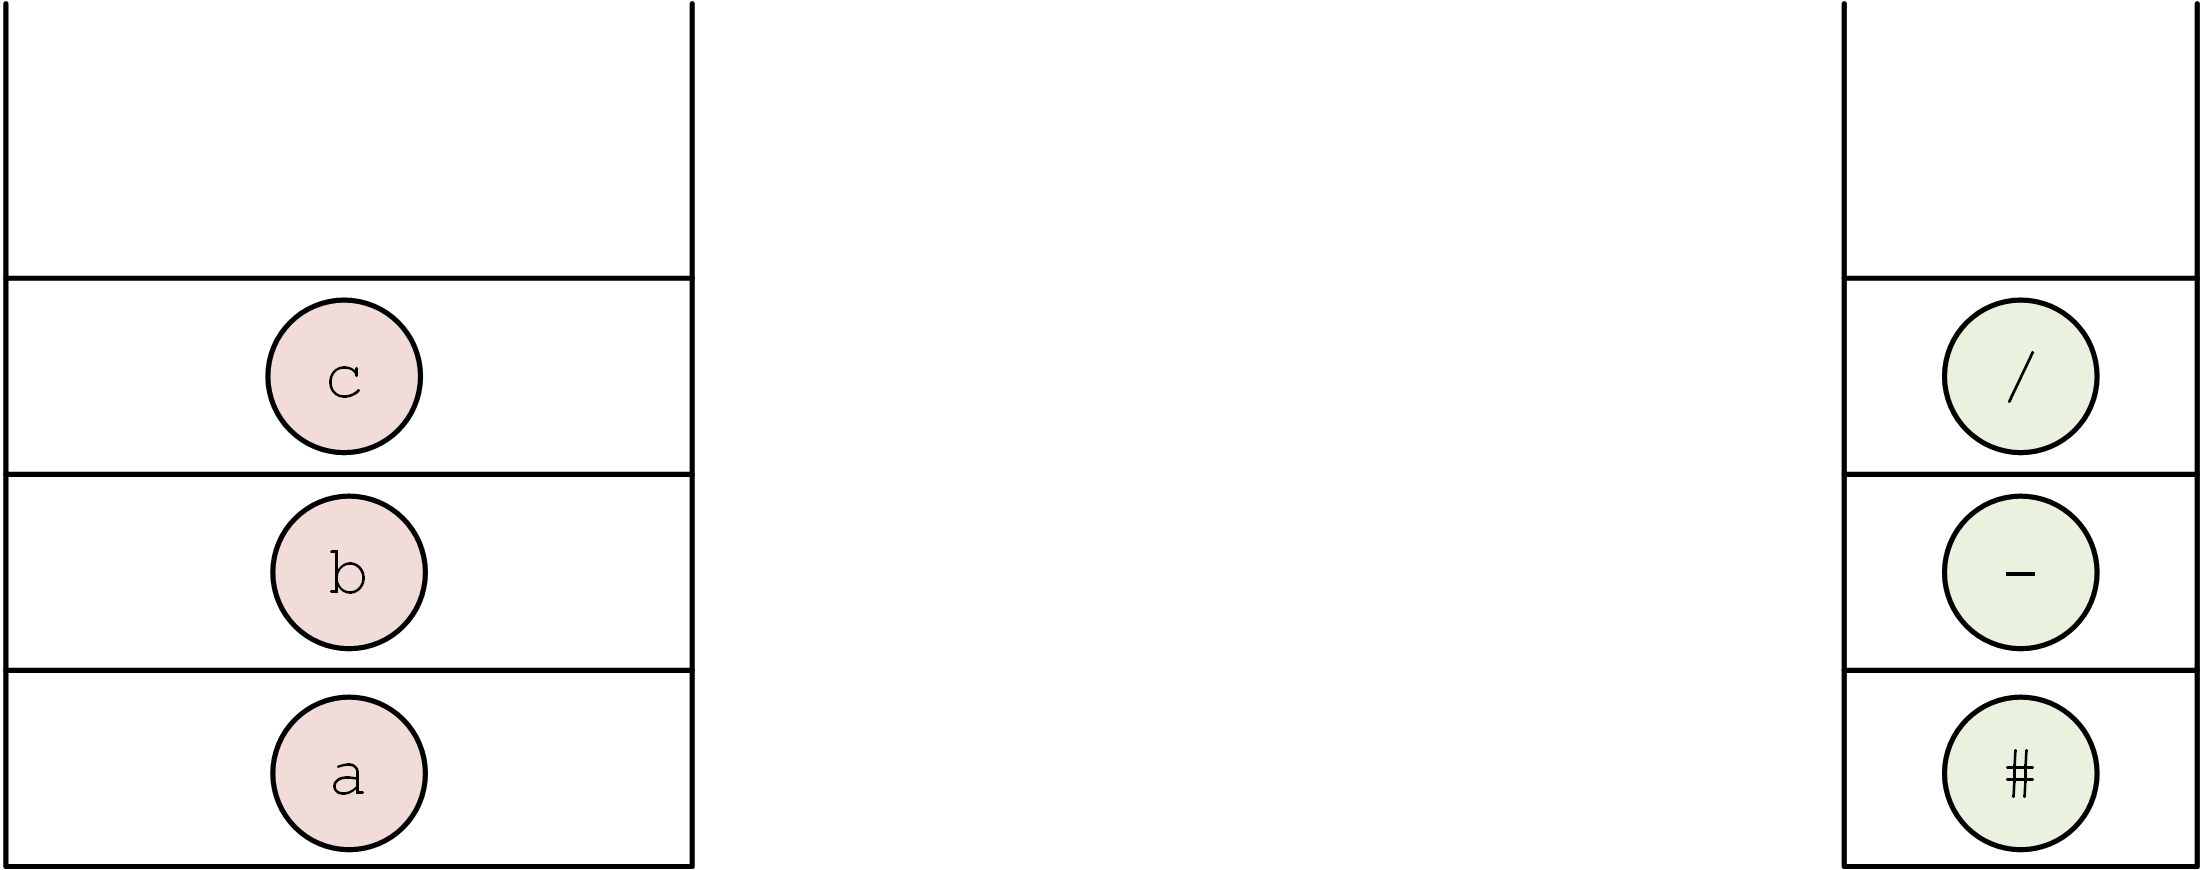
\includegraphics[width=\textwidth]{calculate_6}}
\only<8>{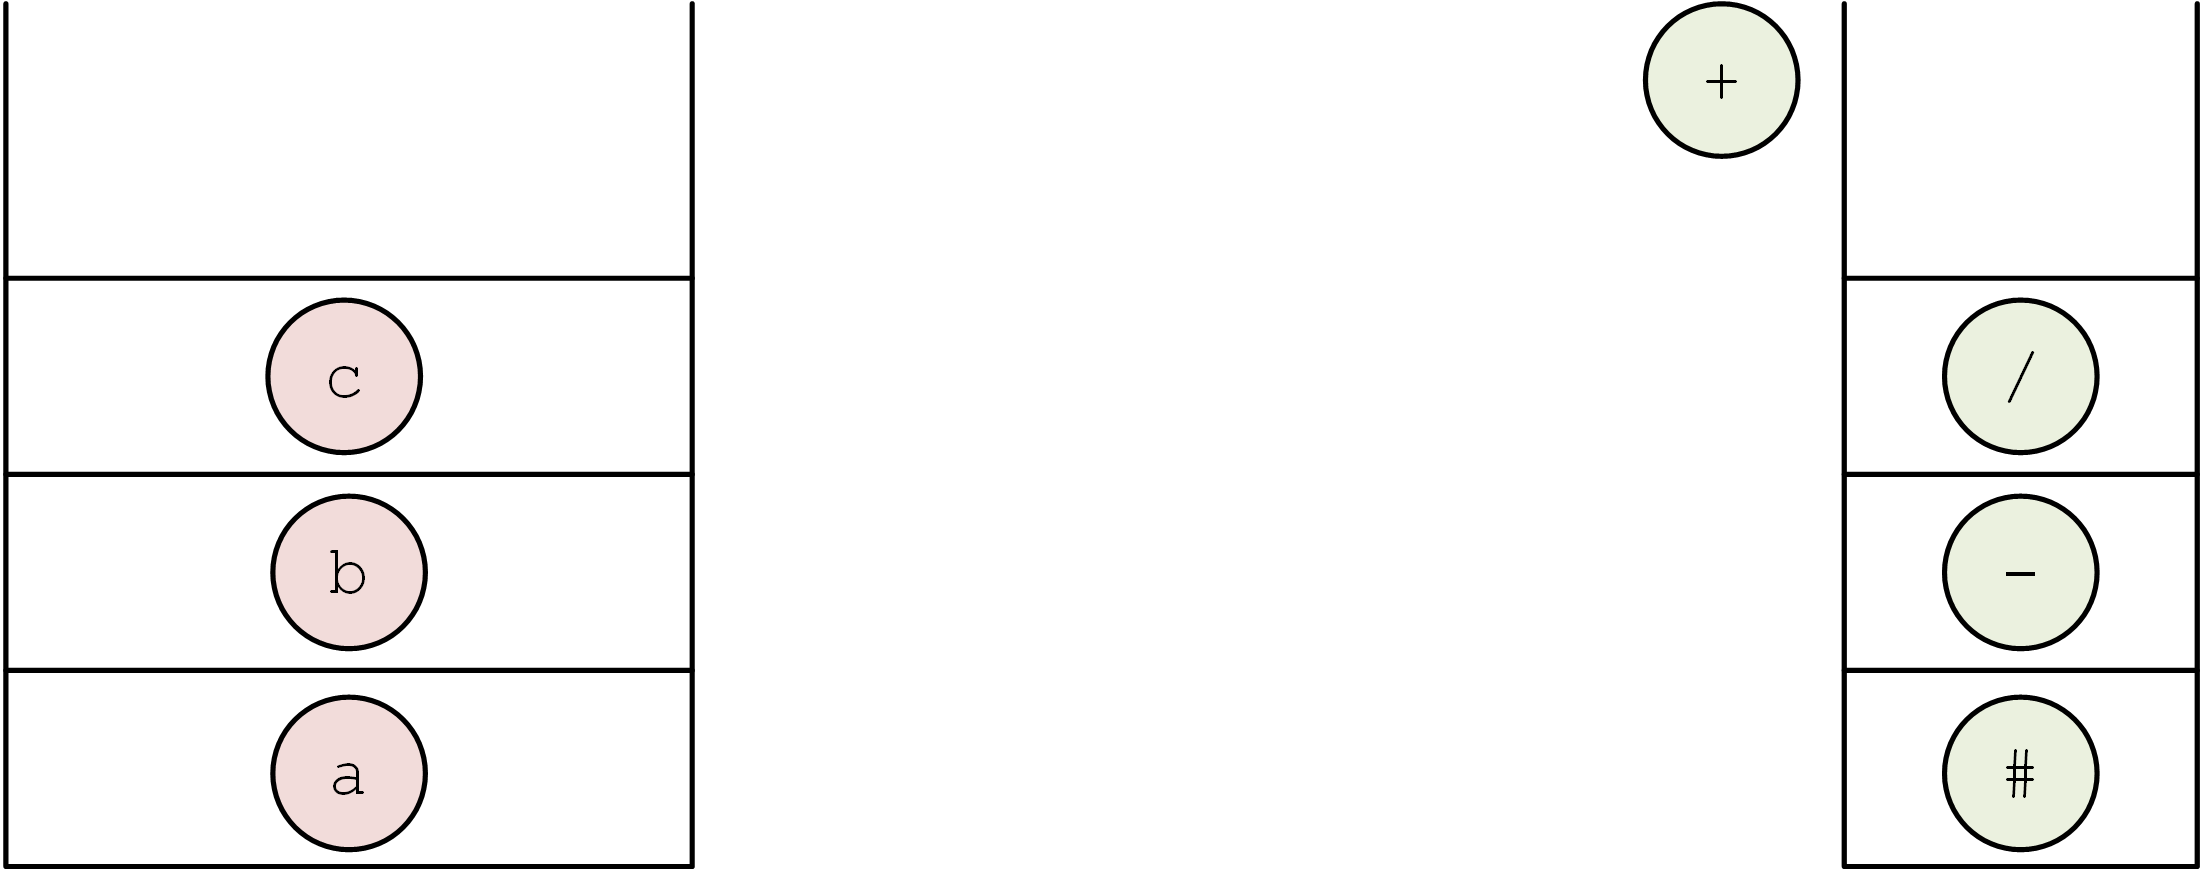
\includegraphics[width=\textwidth]{calculate_7}}
\only<9>{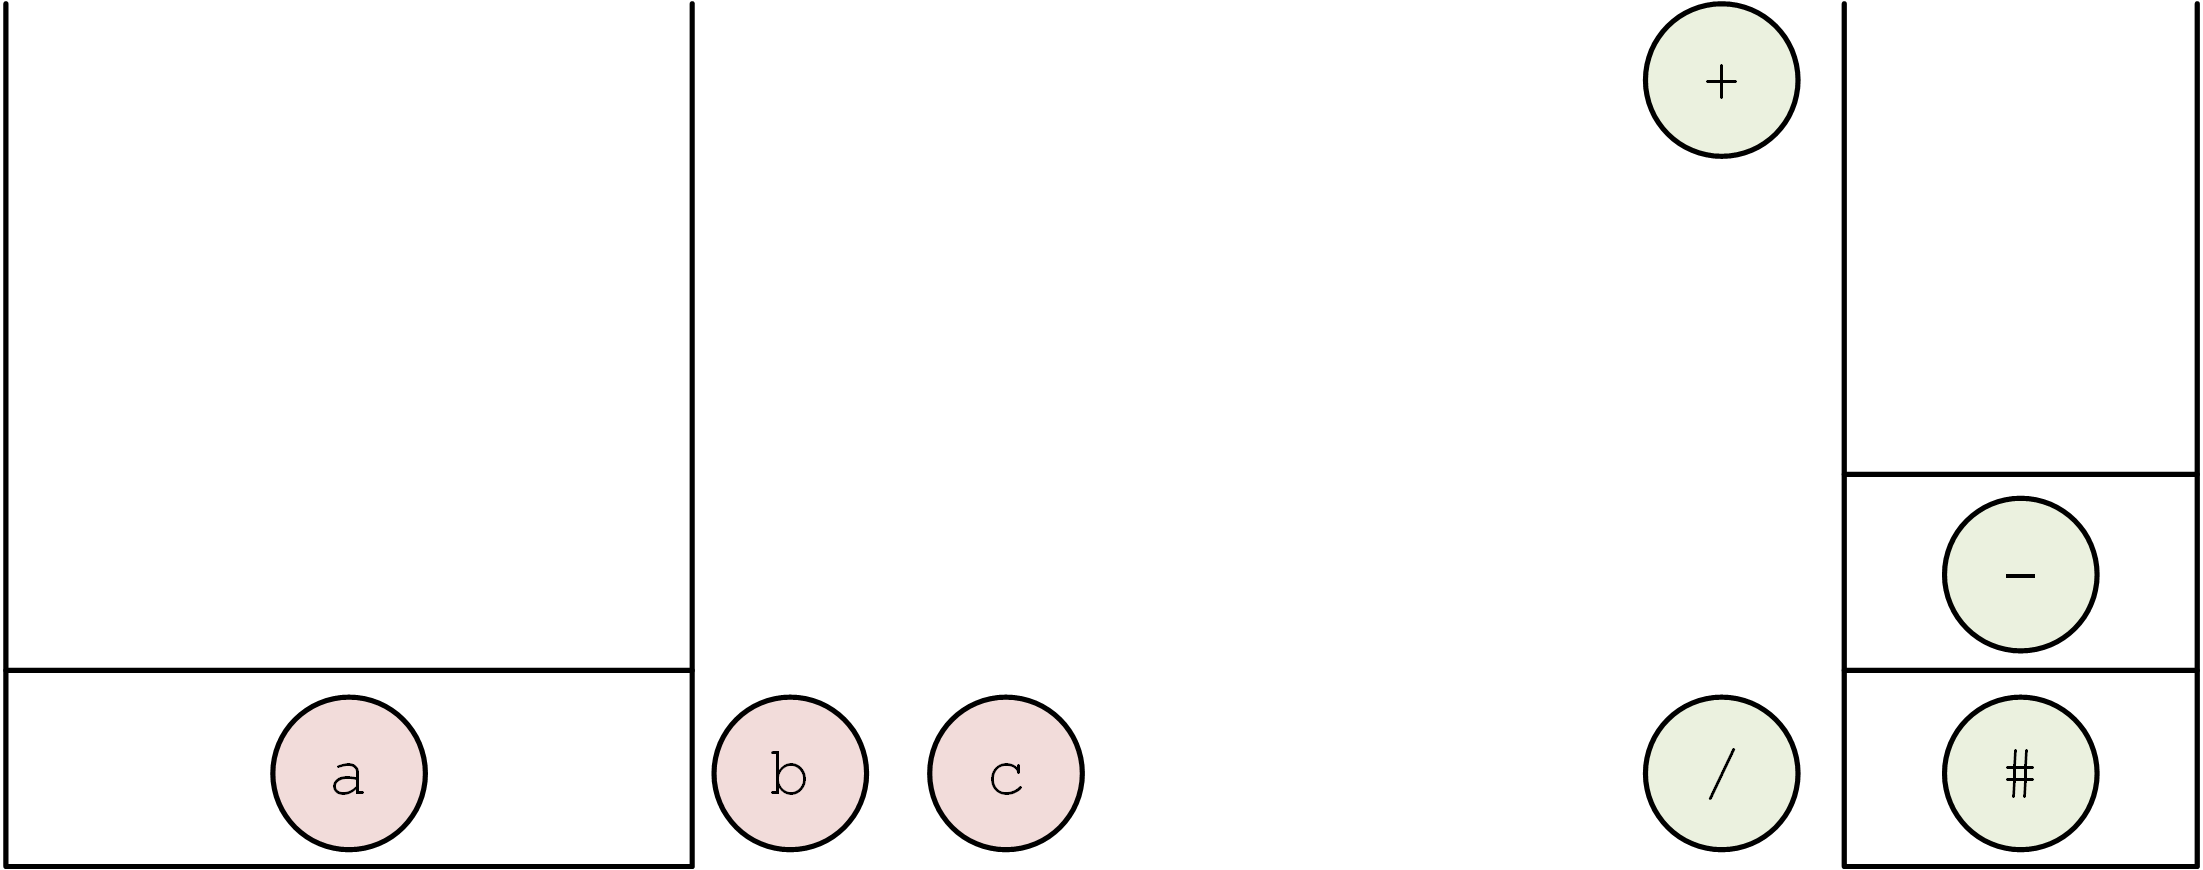
\includegraphics[width=\textwidth]{calculate_8}}
\only<10>{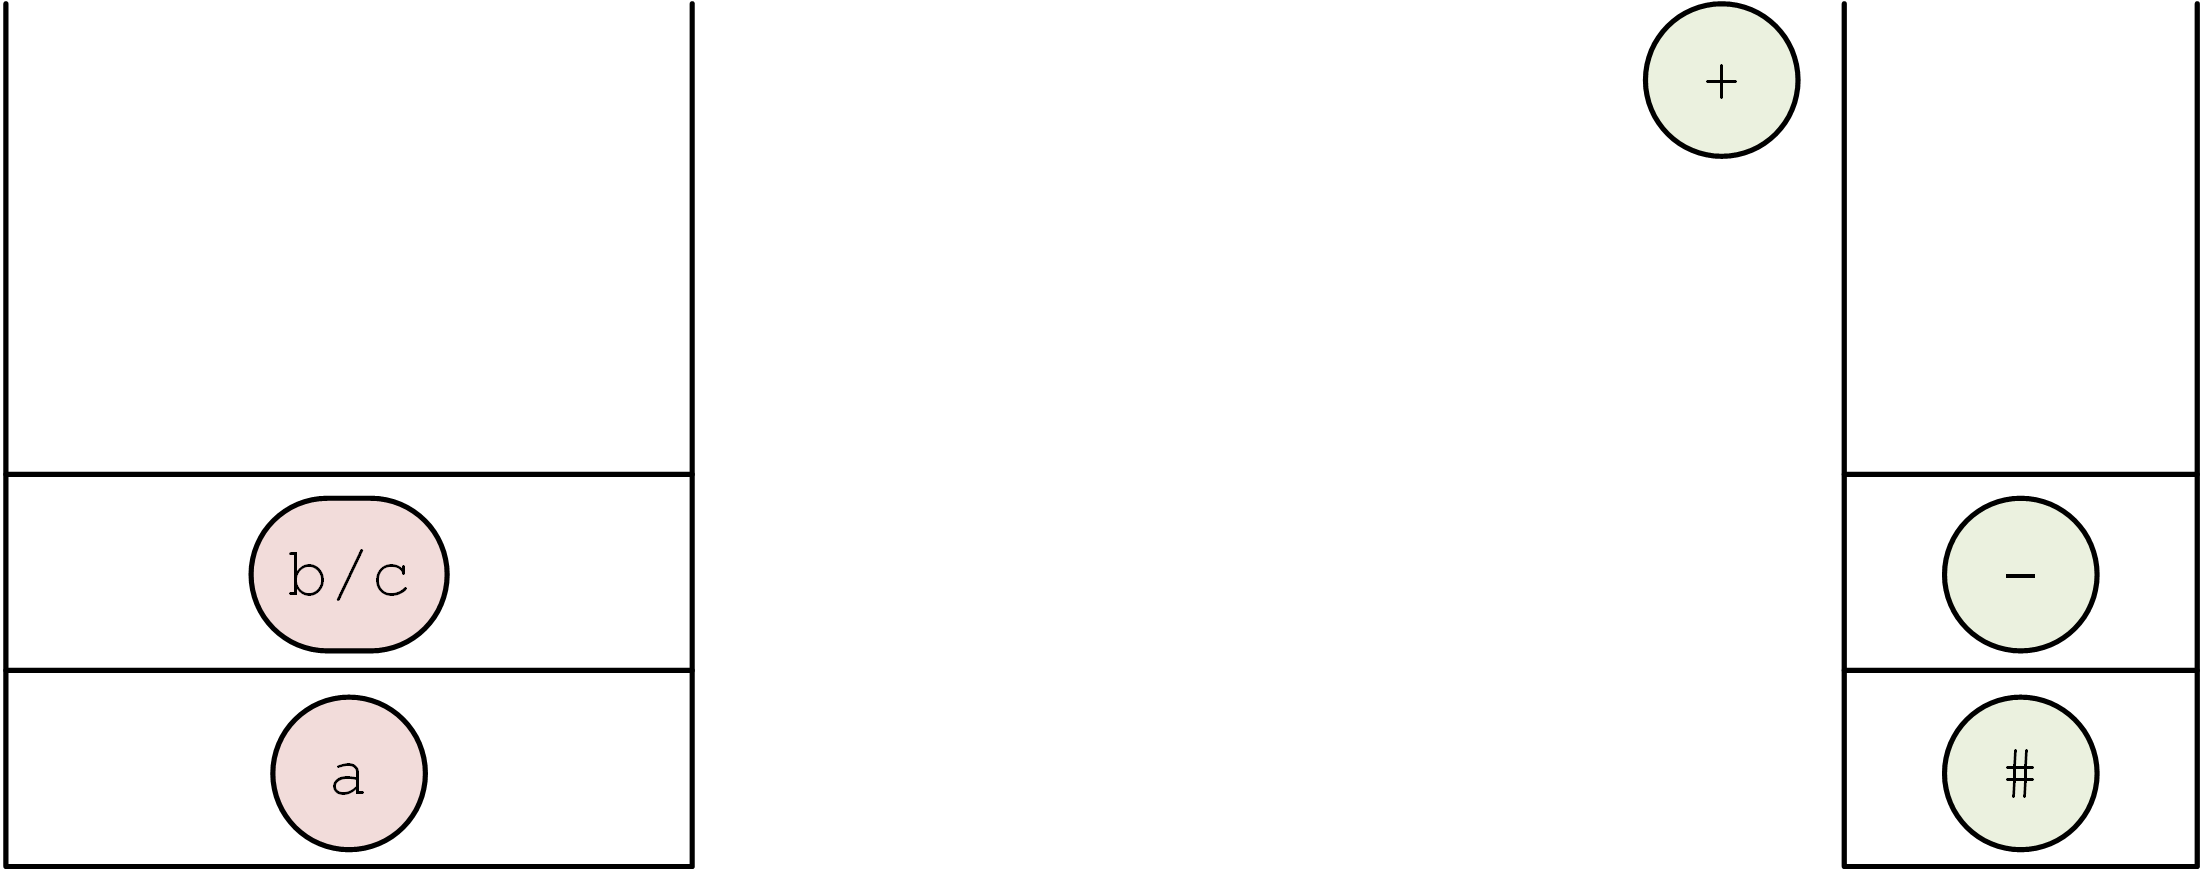
\includegraphics[width=\textwidth]{calculate_9}}
\only<11>{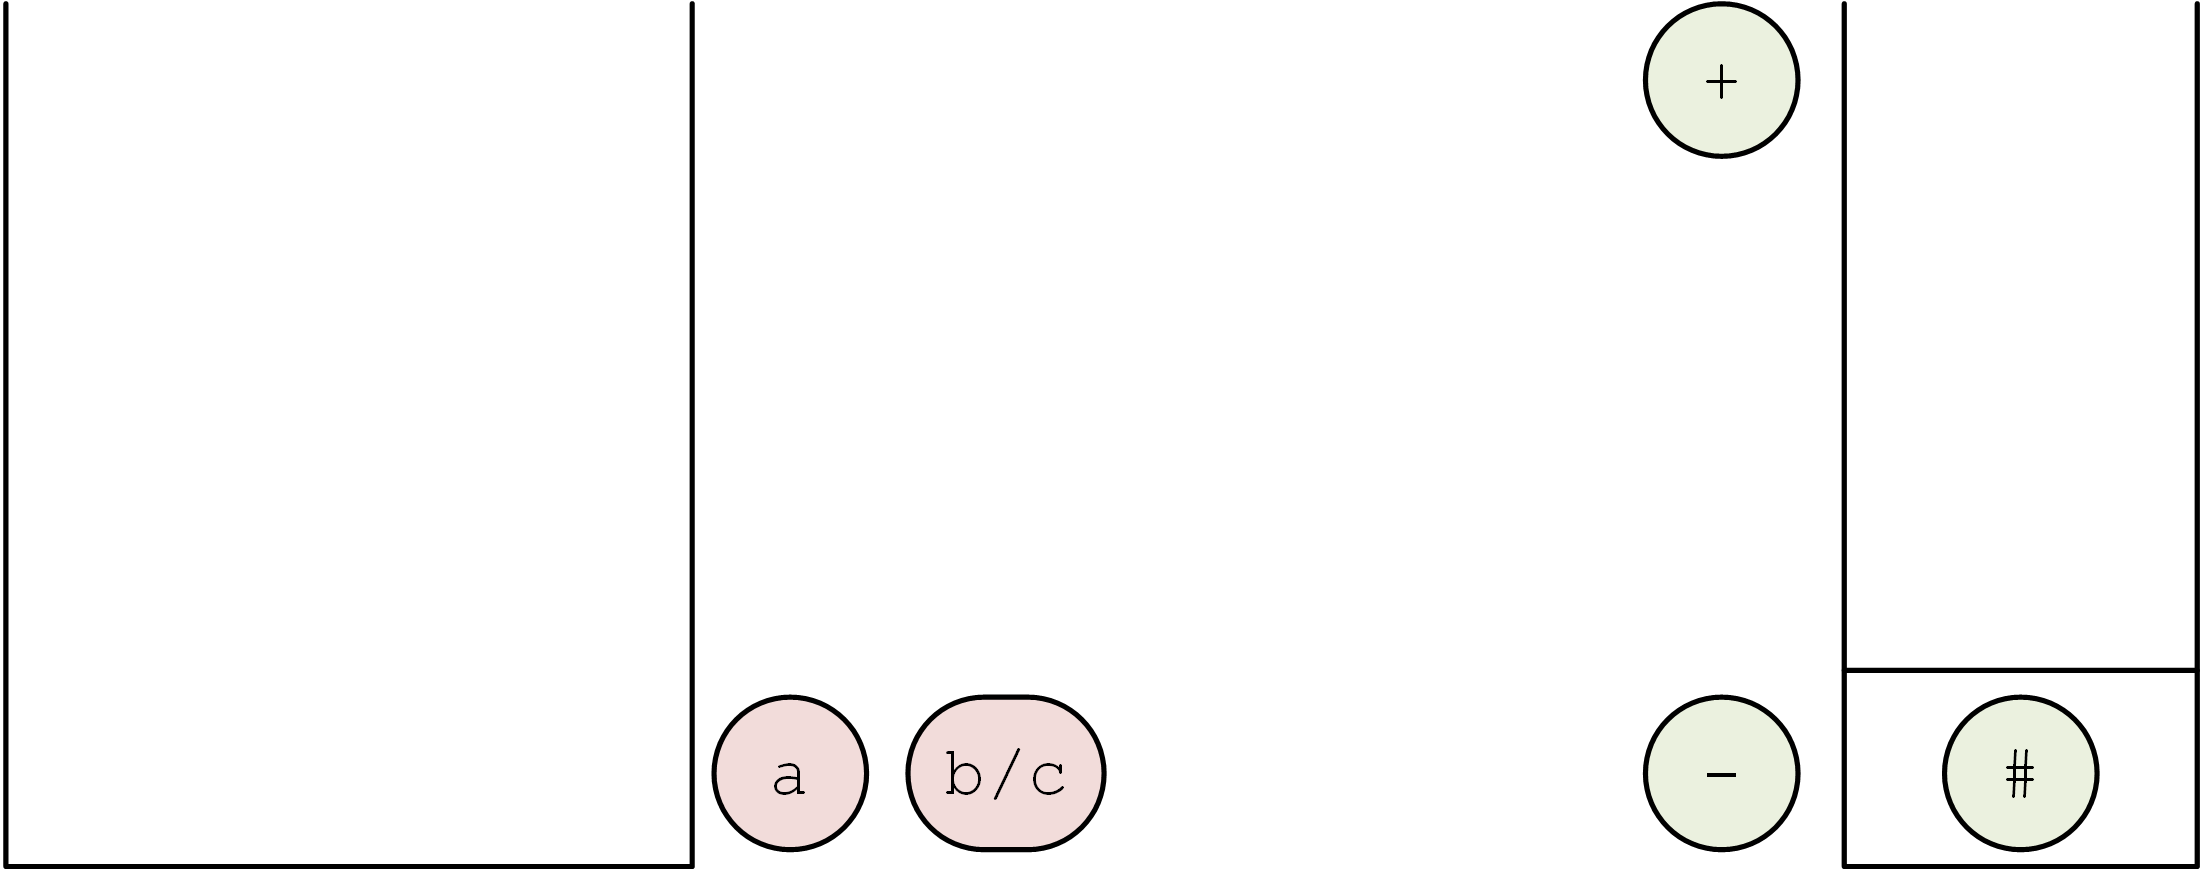
\includegraphics[width=\textwidth]{calculate_10}}
\only<12>{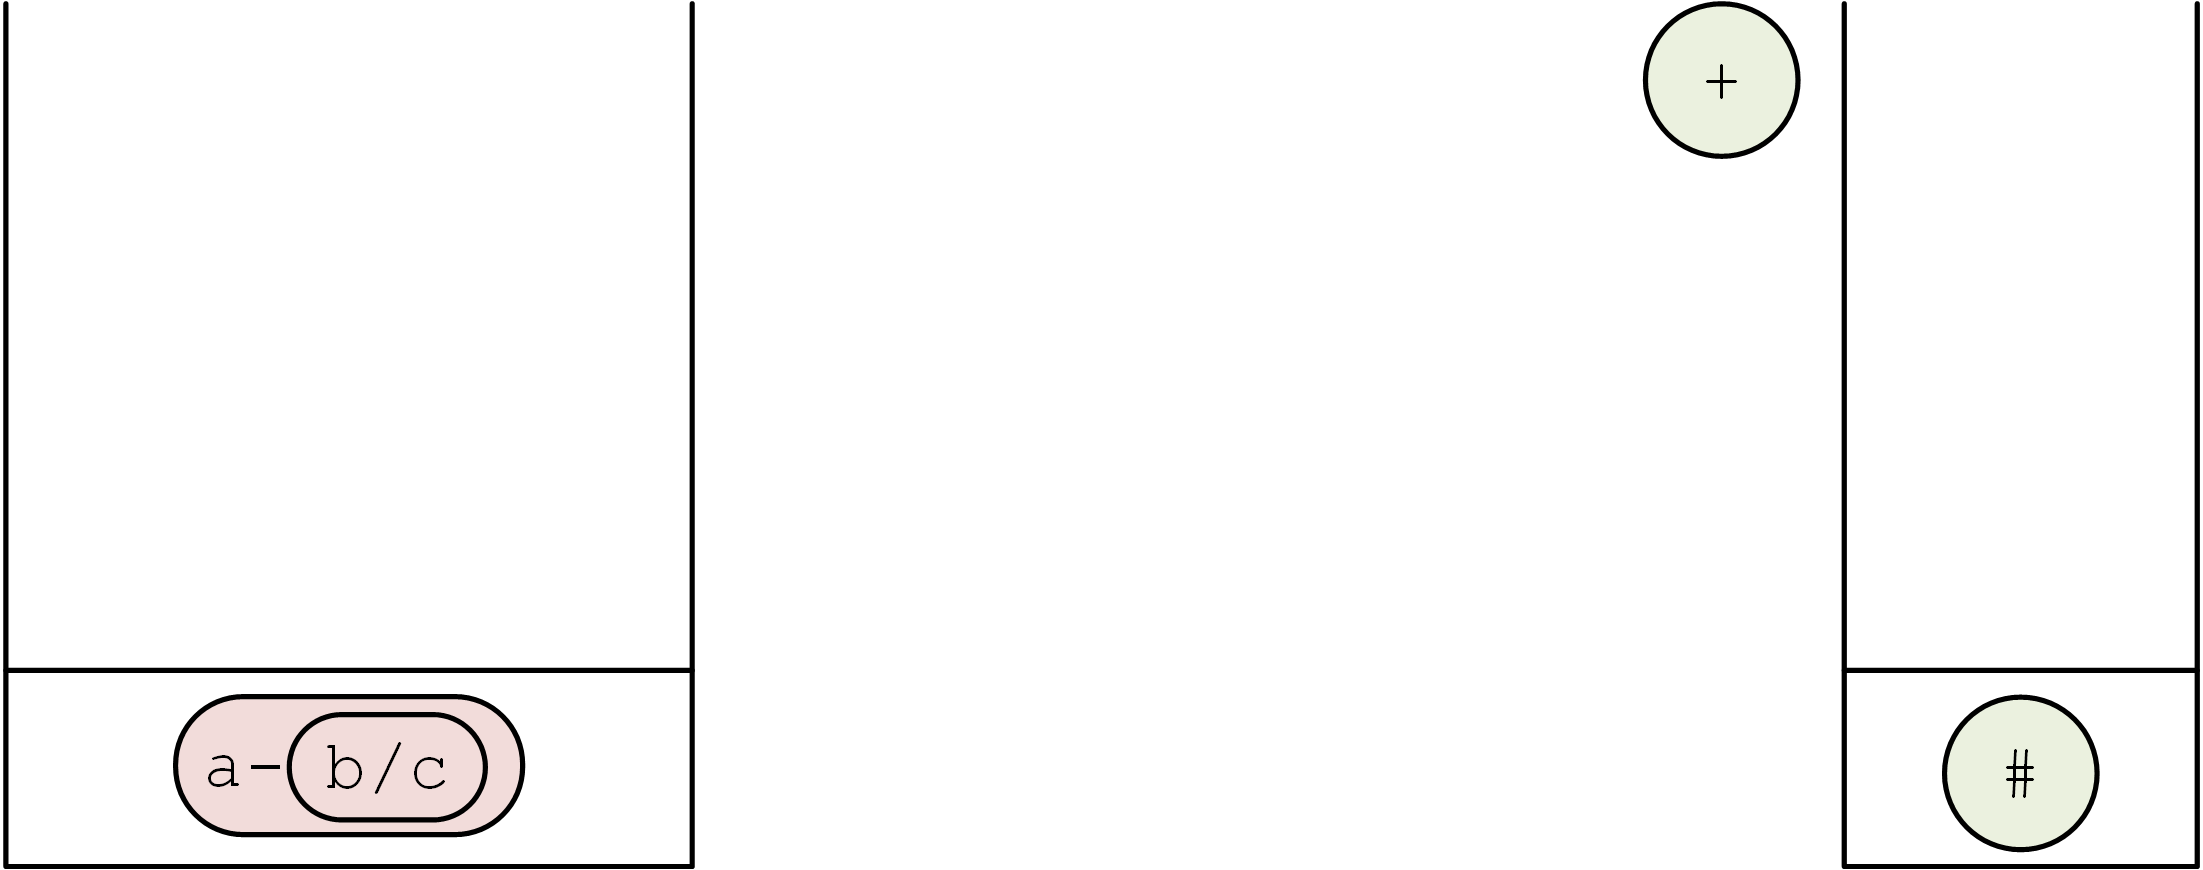
\includegraphics[width=\textwidth]{calculate_11}}
\only<13>{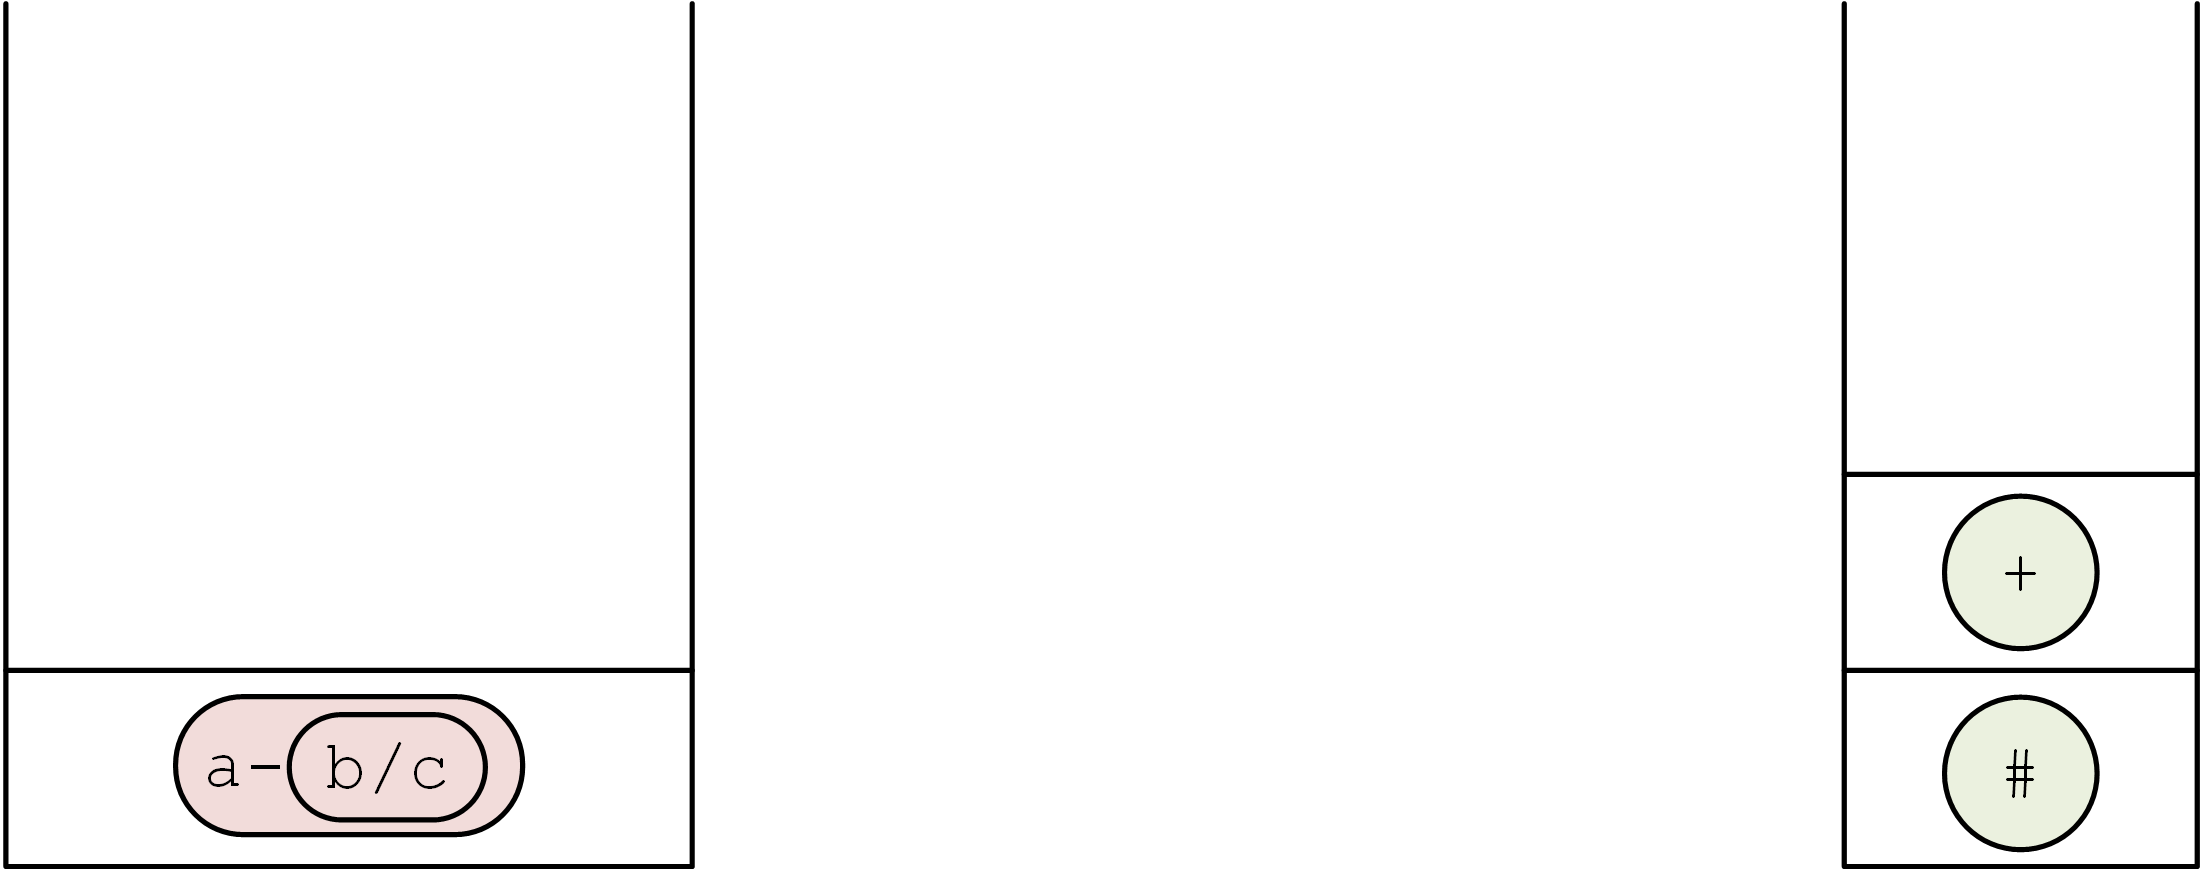
\includegraphics[width=\textwidth]{calculate_12}}
\only<14>{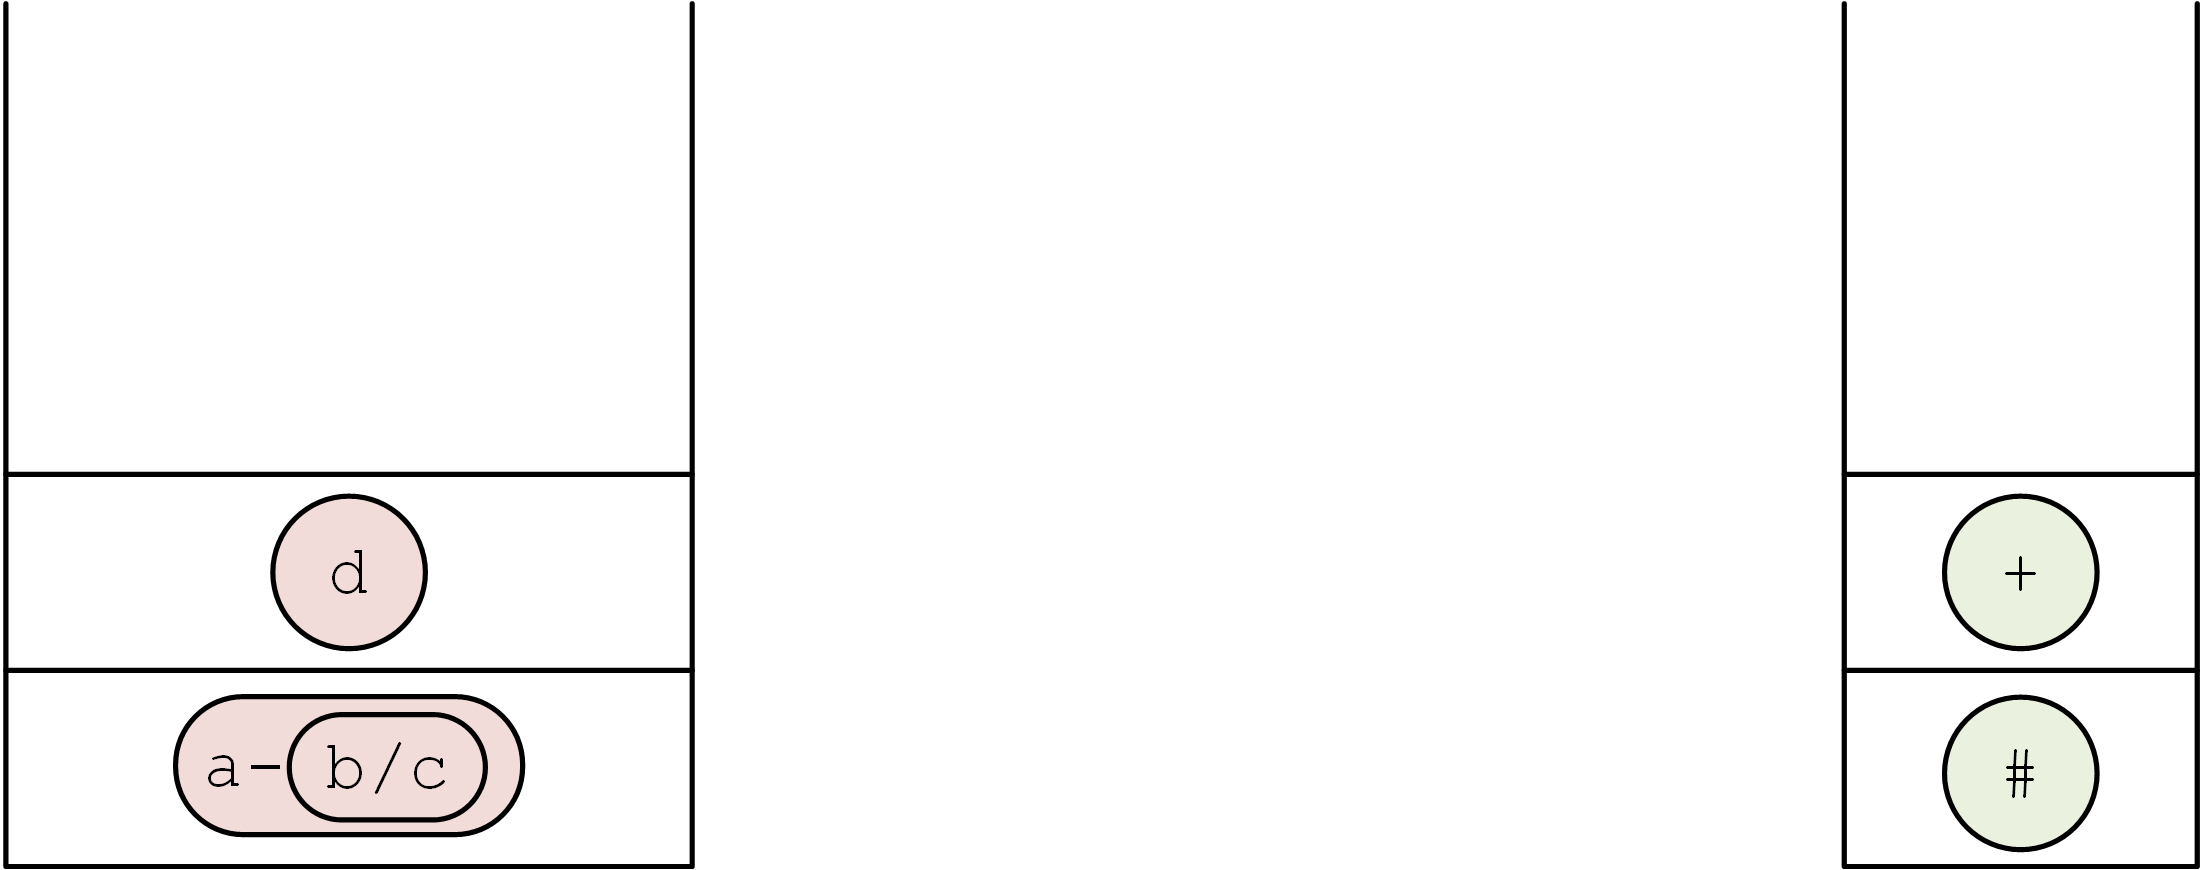
\includegraphics[width=\textwidth]{calculate_13}}
\only<15>{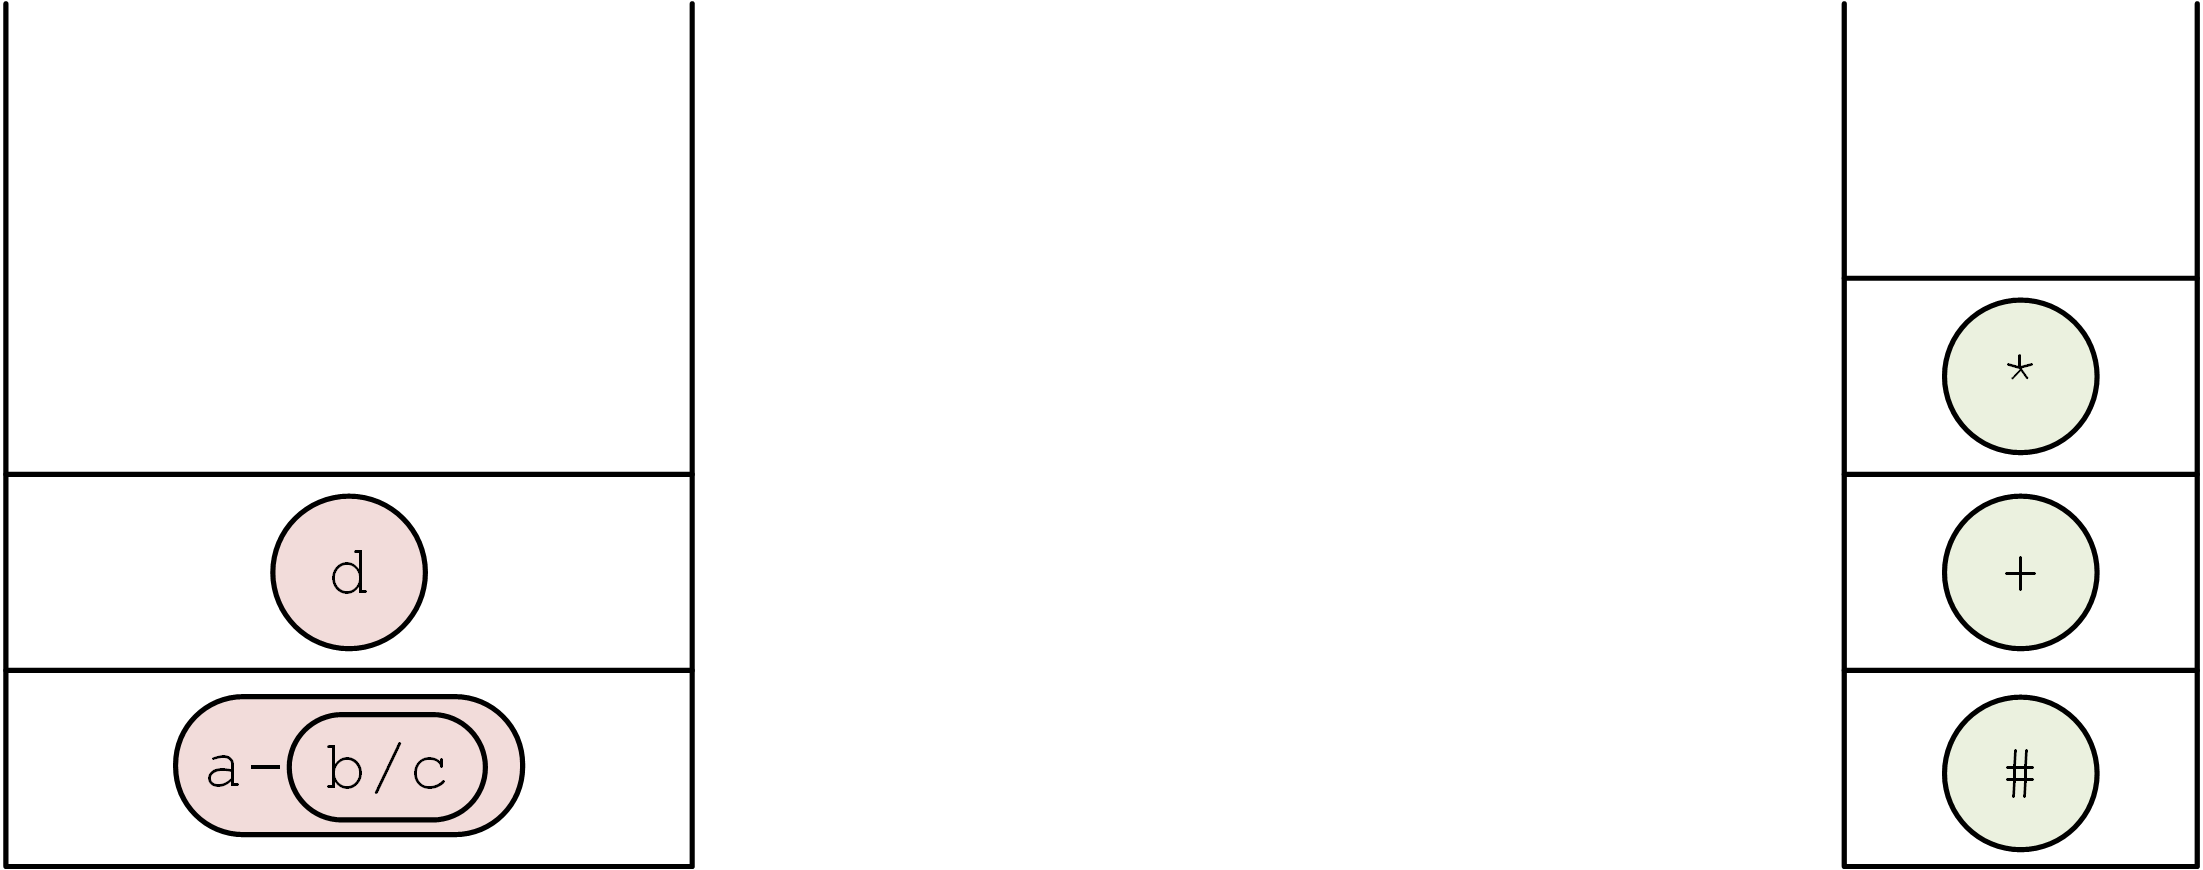
\includegraphics[width=\textwidth]{calculate_14}}
\only<16>{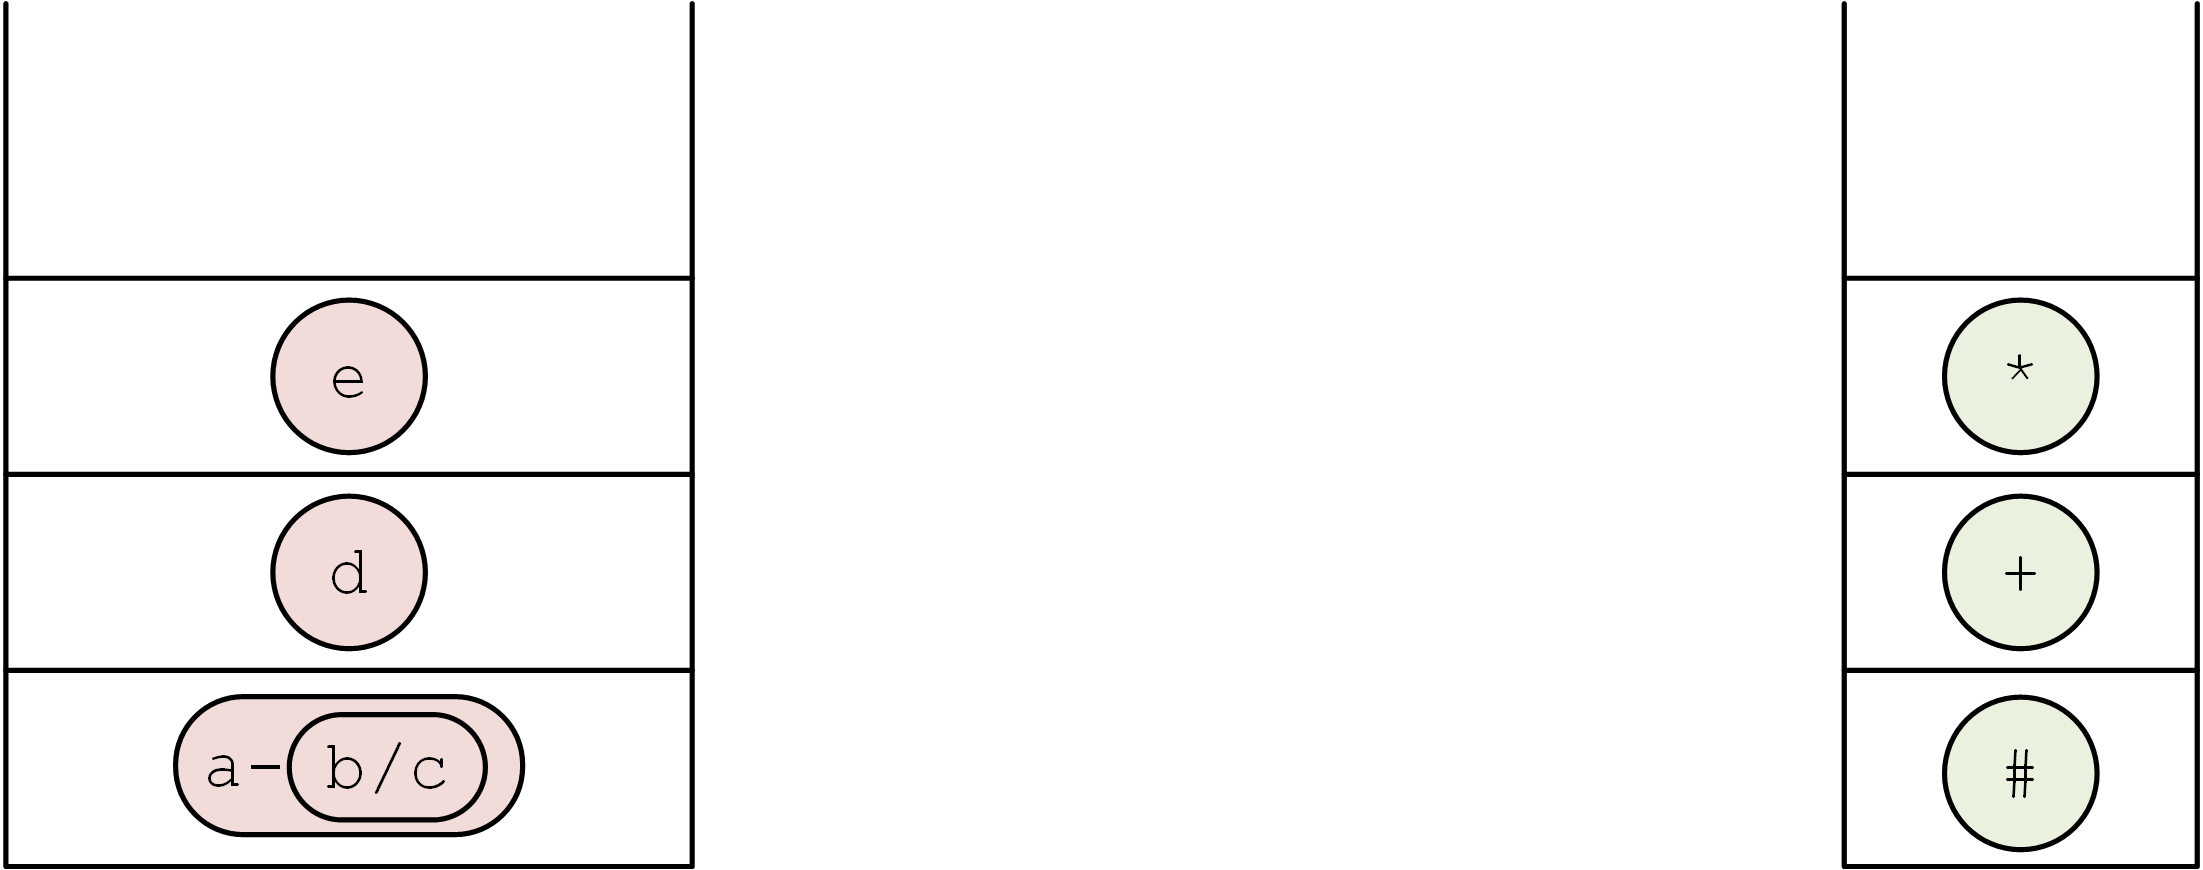
\includegraphics[width=\textwidth]{calculate_15}}
\only<17>{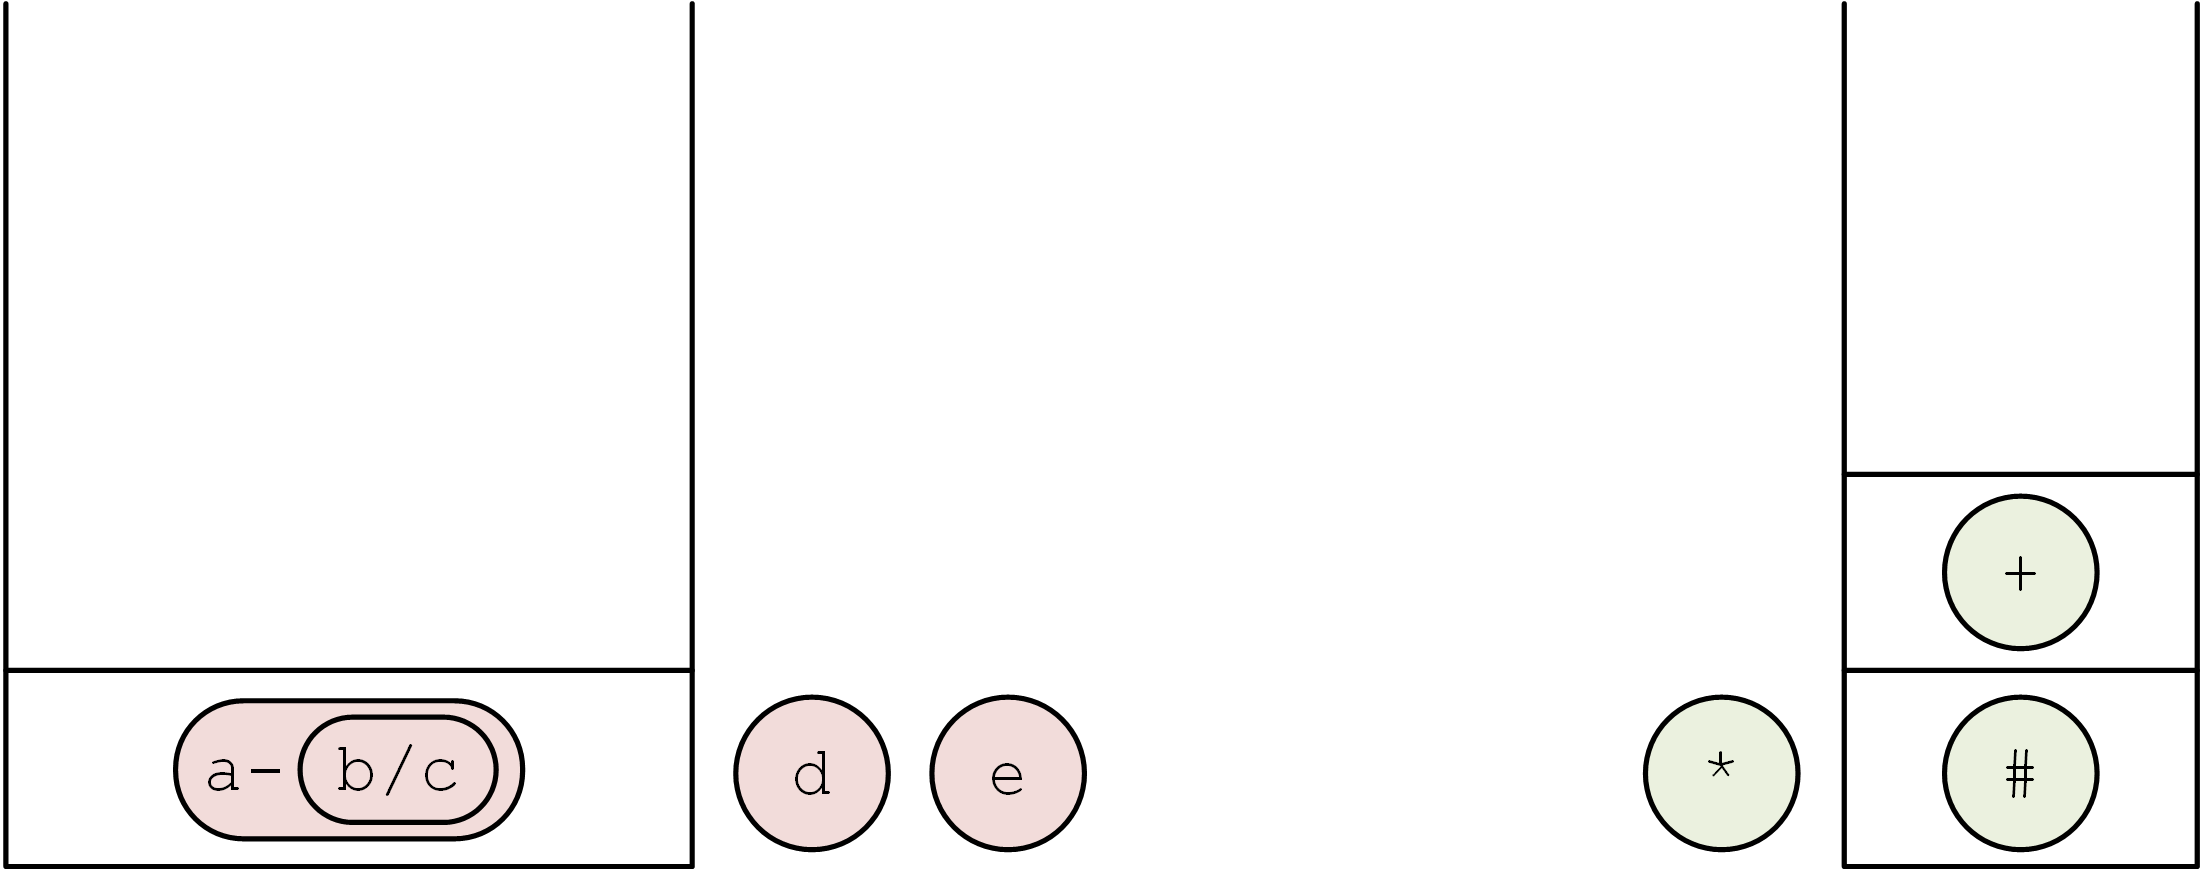
\includegraphics[width=\textwidth]{calculate_16}}
\only<18>{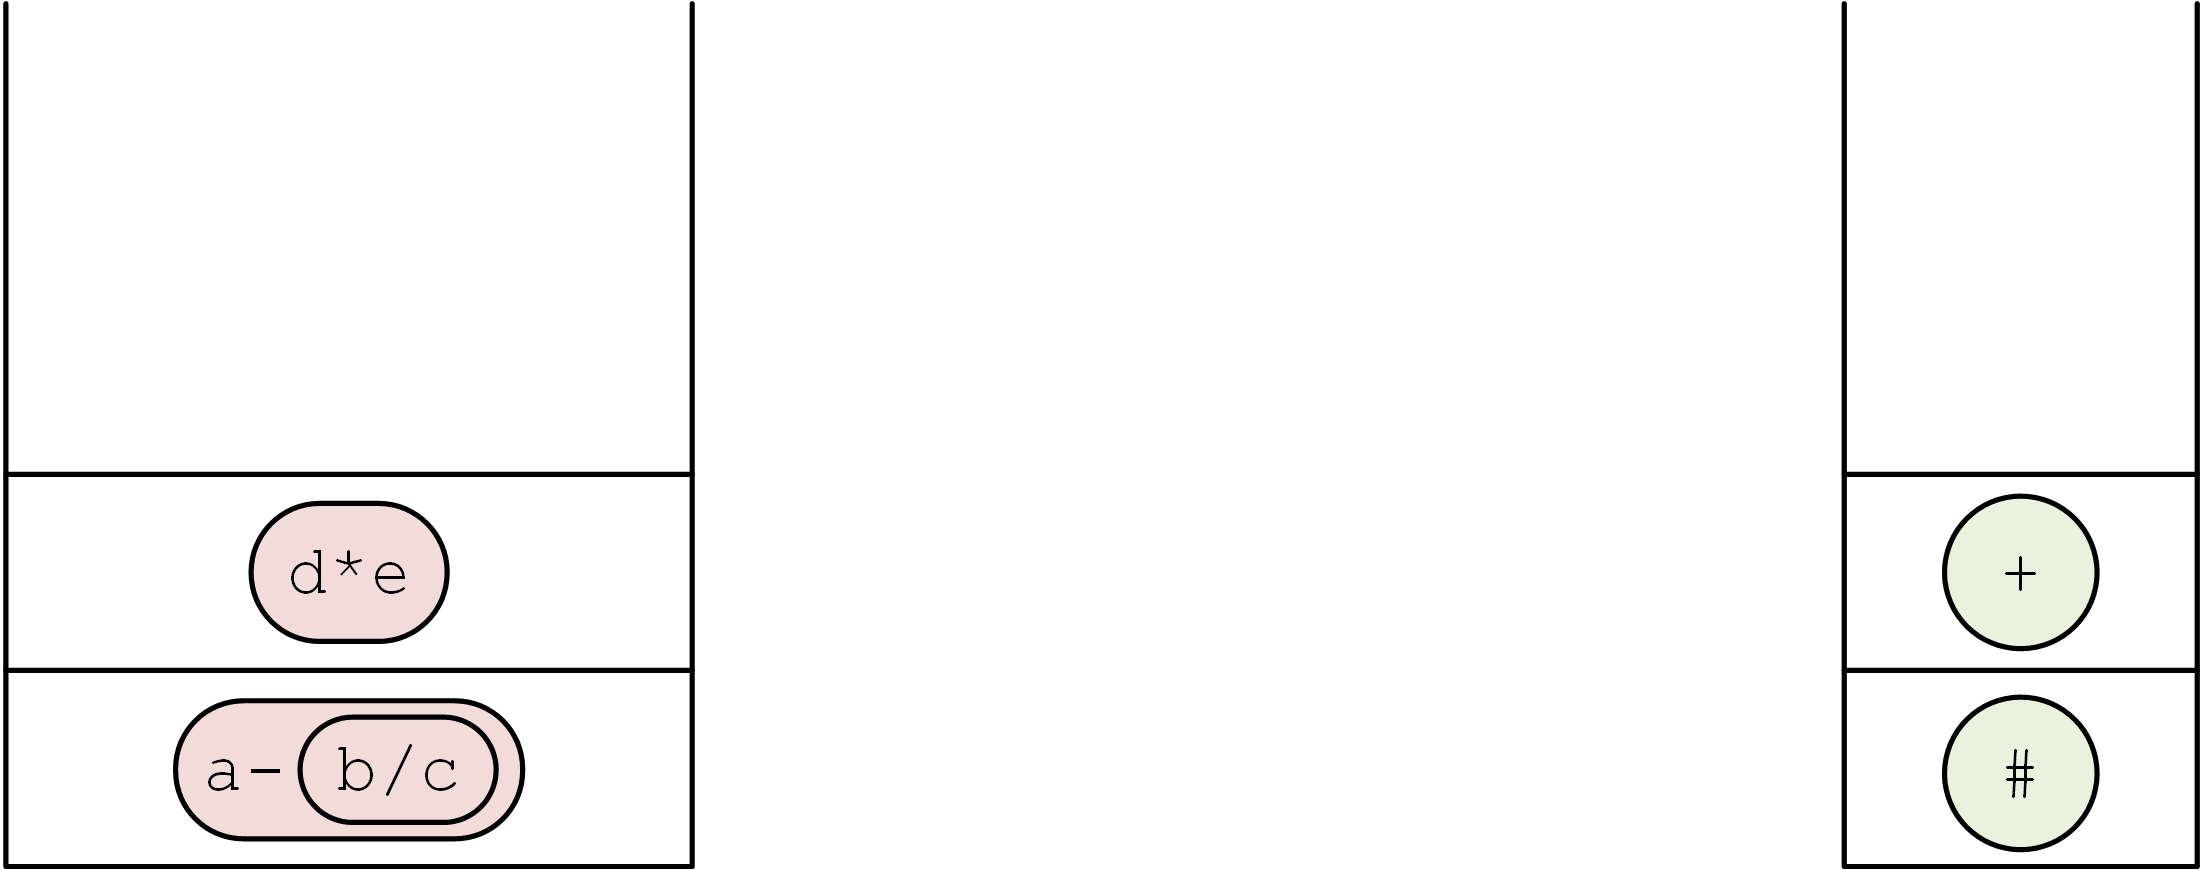
\includegraphics[width=\textwidth]{calculate_17}}
\only<19>{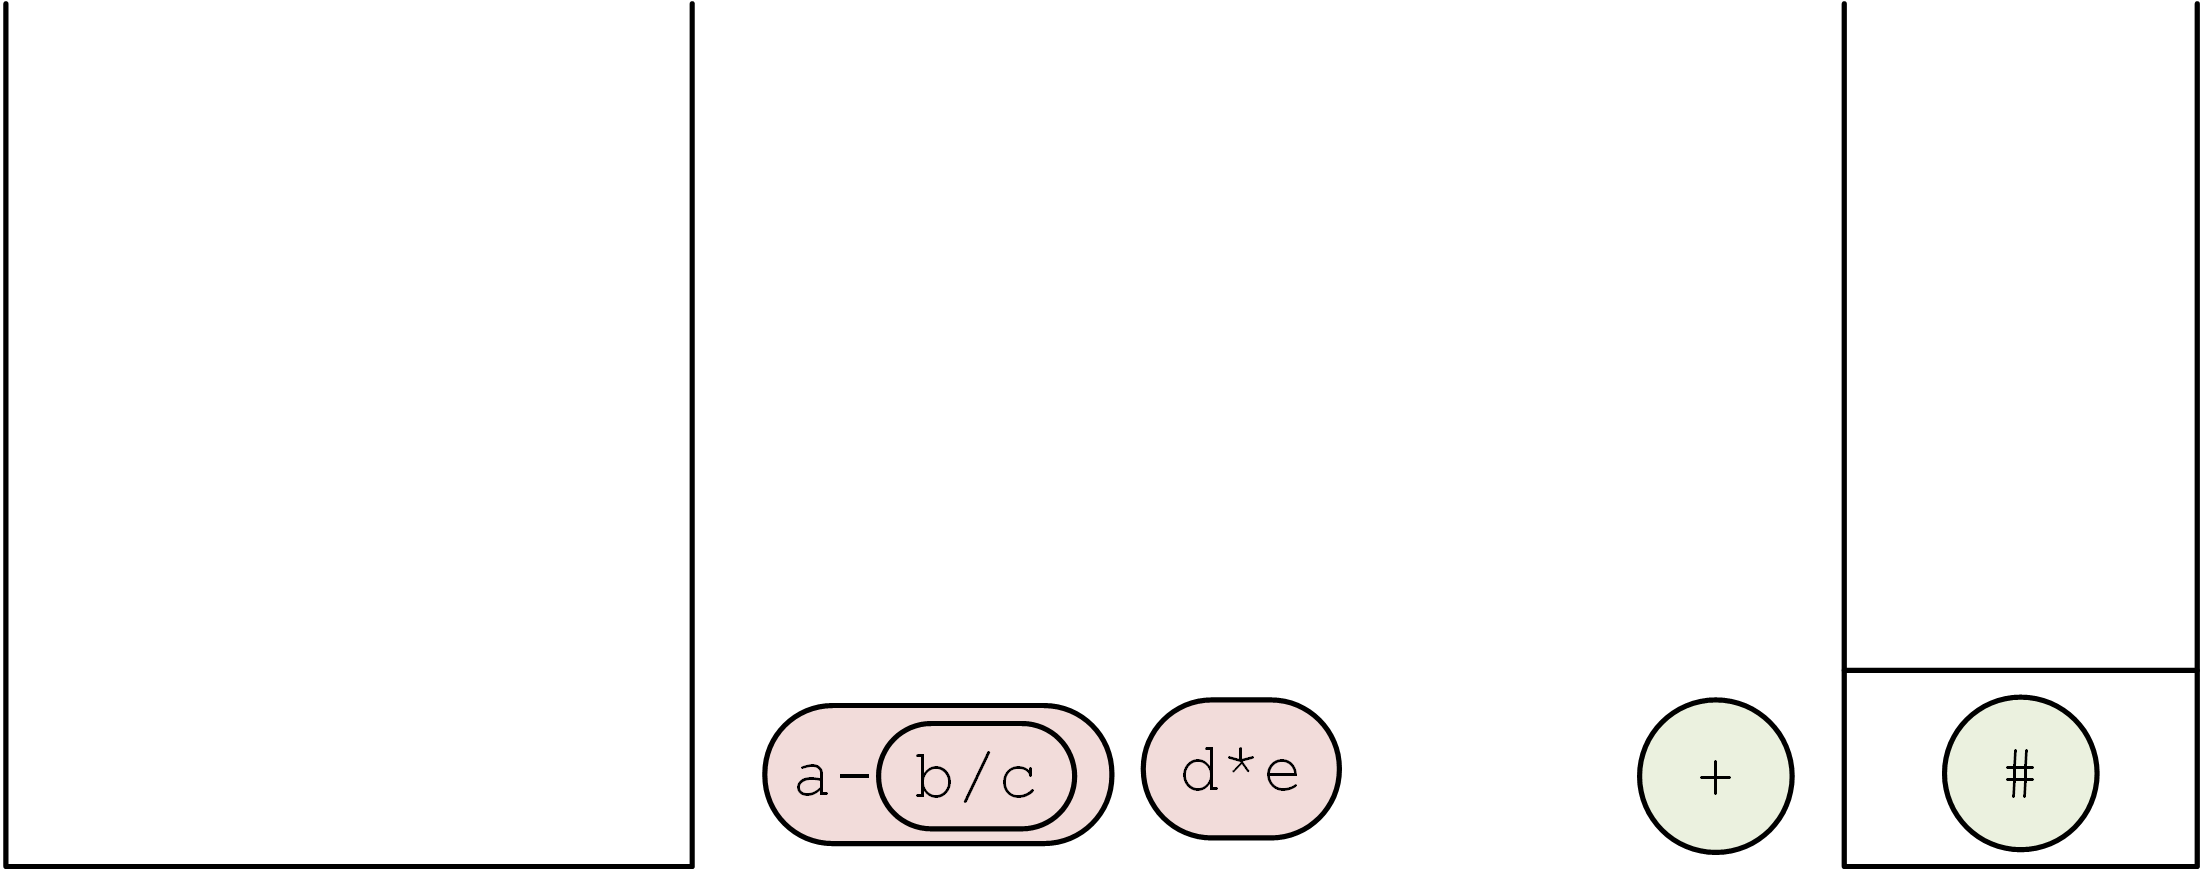
\includegraphics[width=\textwidth]{calculate_18}}
\only<20>{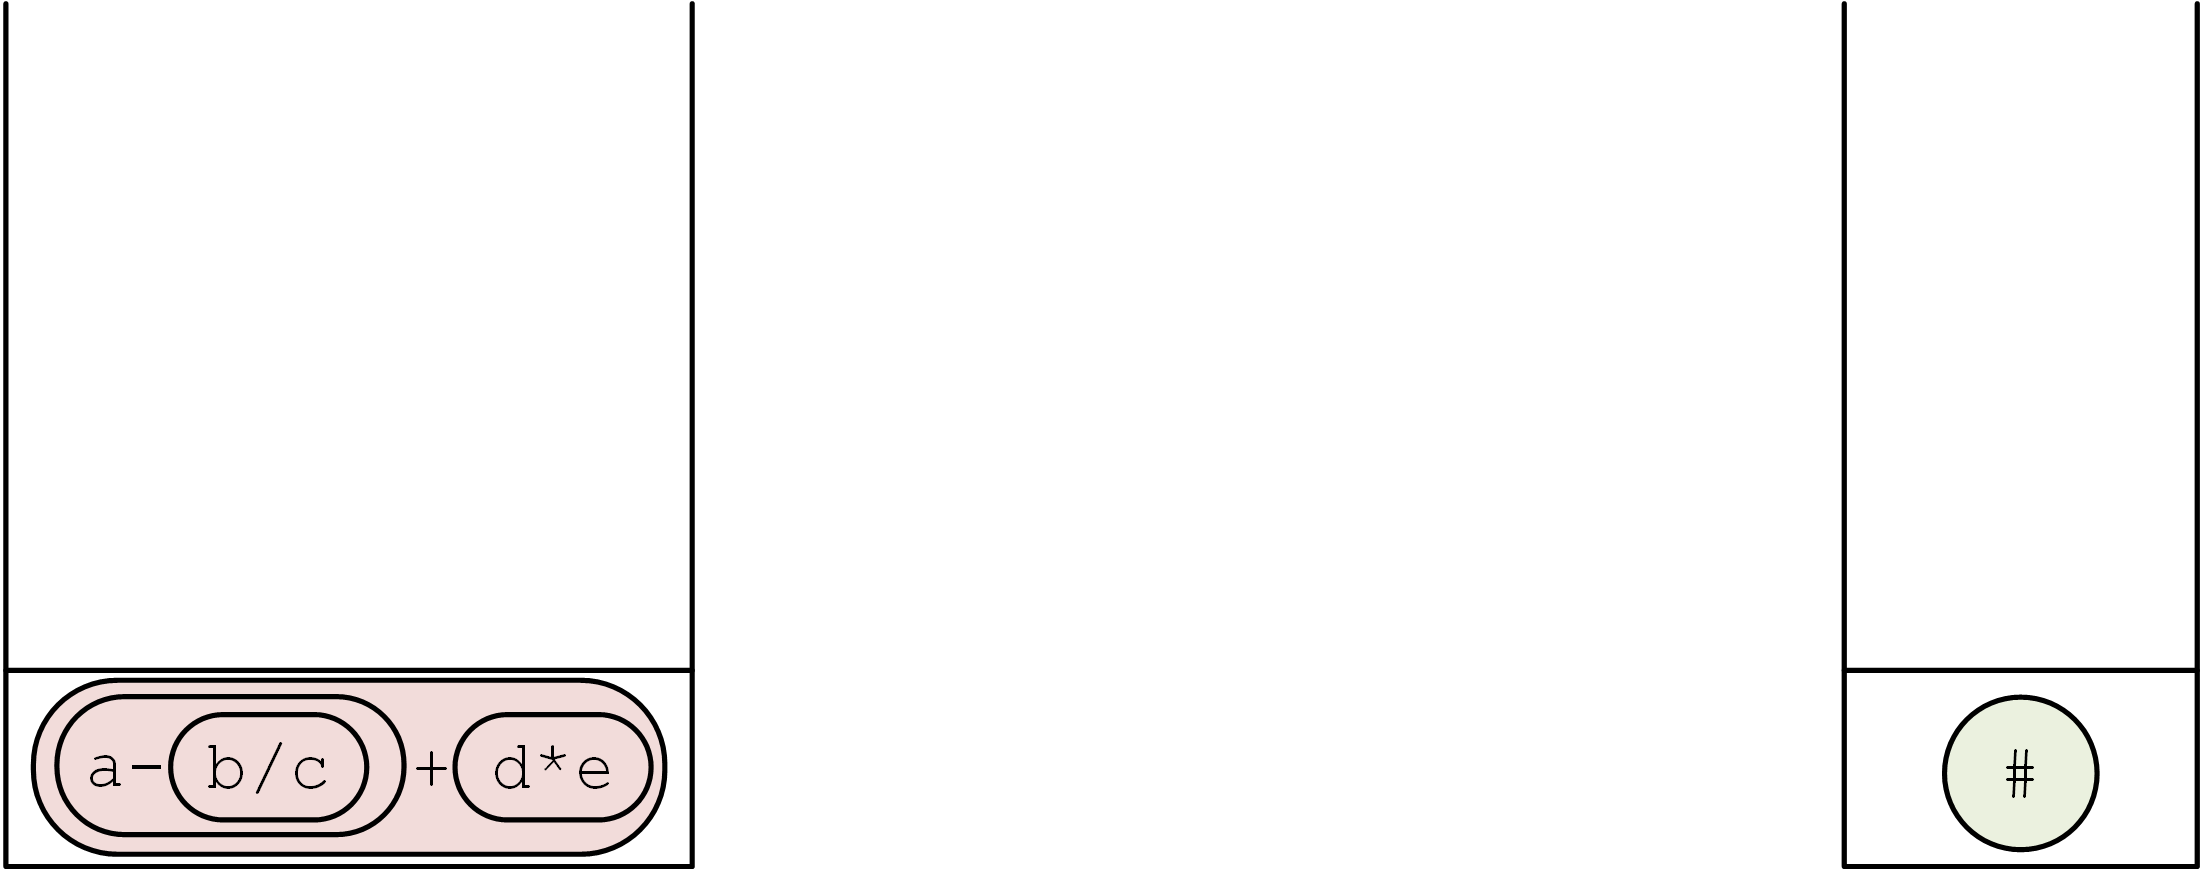
\includegraphics[width=\textwidth]{calculate_19}}
\only<21->{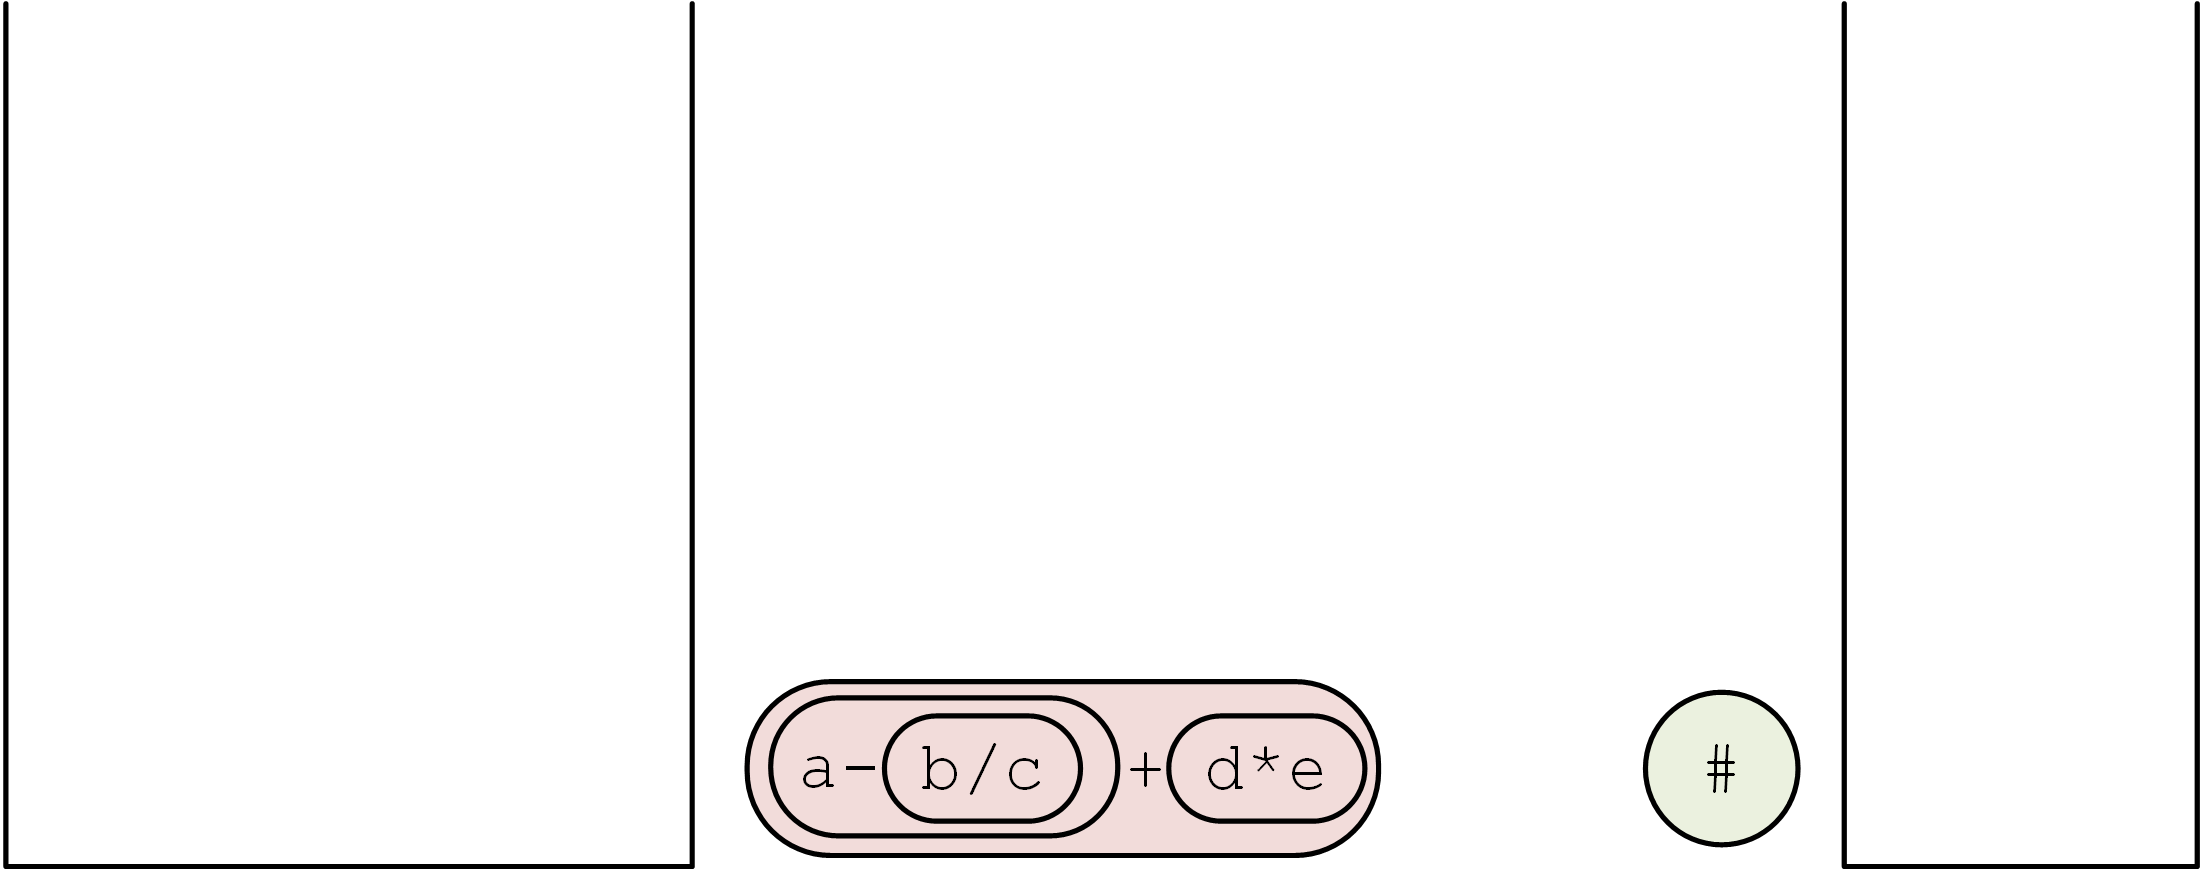
\includegraphics[width=\textwidth]{calculate_20}}

\end{frame}

%-----------------

\begin{frame}[fragile]{8.4.2~简单计算器}

简单四则运算的类代码清单如下:
\begin{blueblock}{\texttt{Calculator}类定义部分一}
\vspace{-2.5mm}\begin{lstlisting}[moreemph={Calculator,const\_iterator,Stack},numbers=left,xleftmargin=2em,framexleftmargin=2em]
class Calculator {
private:
    Stack<double> m_num;                          //操作数栈
    Stack<char> m_opr;                            //运算符栈
    int precedence(const char &s ) const;         //获取运算符优先级
    double readNum(string::const_iterator &it);   //读取操作数
    void calculate();                             //取出运算符和操作数进行计算
                                                  //内联函数,判断是否为数字
    bool isNum(string::const_iterator &c) const {
        return* c >= ’0’&& * c <= ’9’ || * c == ’.’;
    }
public:
    Calculator(){ m_opr.push(’#’); }              //运算符栈初始化
    double doIt(const string &exp);               //表达式求值
};

\end{lstlisting}\vspace{-2.5mm}
\end{blueblock}


\end{frame}

%-----------------

\begin{frame}[fragile]{8.4.2~简单计算器}

简单四则运算的类代码清单如下:
\begin{blueblock}{\texttt{Calculator}类定义部分二}
\vspace{-2.5mm}\begin{lstlisting}[moreemph={Calculator,const\_iterator,Stack},firstnumber=17,numbers=left,xleftmargin=2em,framexleftmargin=2em]
int Calculator::precedence(const char & s) const{
    switch (s) {
        case ’=’: return 0;
        case ’#’: return 1;
        case ’+’: case ’-’: return 2;
        case ’*’: case ’/’: return 3;
    }
}
double Calculator::readNum(string::const_iterator &it){
    string t;
    while (isNum(it))
        t += *it++;                  //继续扫描,直到遇到运算符
    return stod(t);              //将数字字符串转换为double类型(C++11新特性)
}
\end{lstlisting}\vspace{-2.5mm}
\end{blueblock}


\end{frame}

%-----------------

\begin{frame}[fragile]{8.4.2~简单计算器}

简单四则运算的类代码清单如下:
\begin{blueblock}{\texttt{Calculator}类定义部分三}
\vspace{-2.5mm}\begin{lstlisting}[moreemph={Calculator,const\_iterator,Stack},firstnumber=31,numbers=left,xleftmargin=2em,framexleftmargin=2em]
void Calculator::calculate(){
    double b = m_num.top();                //取出右操作数
    m_num.pop();                           //右操作数出栈
    double a = m_num.top();                //取出左操作数
    m_num.pop();                           //左操作数出栈
    if (m_opr.top() == ’+’)
        m_num.push(a + b);                 //将计算结果压栈,下面三个运算与此操作相同
    else if (m_opr.top() == ’-’)
        m_num.push(a - b);
    else if (m_opr.top() == ’ * ’)
        m_num.push(a*b);
    else if (m_opr.top() == ’/’)
        m_num.push(a / b);
    m_opr.pop();                           //当前运算结束,运算符出栈
}
\end{lstlisting}\vspace{-2.5mm}
\end{blueblock}


\end{frame}

%-----------------

\begin{frame}[fragile]{8.4.2~简单计算器}

简单四则运算的类代码清单如下:
\begin{blueblock}{\texttt{Calculator}类定义部分四}
\vspace{-2.5mm}\begin{lstlisting}[moreemph={Calculator,const\_iterator,Stack},firstnumber=46,numbers=left,xleftmargin=2em,framexleftmargin=2em]
double Calculator::doIt(const string & exp){
    m_num.clear();                  //保证同一个对象再次调用doIt时数据栈为空
    for (auto it = exp.begin(); it != exp.end();) {
        if (isNum(it))              //遇到操作数
            m_num.push(readNum(it));//操作数入栈
        else{                       //遇到运算符,下面while循环条件中不能忽略优先级相同的情况
            while (precedence( * it) <= precedence(m_opr.top())){
                if (m_opr.top() == ’#’)
                    break;          //如果运算符栈只剩下#,则计算完毕
                calculate();        //执行栈顶运算符计算
            }
            if ( * it != ’=’)
                m_opr.push( * it);  //运算符入栈
            ++it;                   //继续扫描
        }
    }
    return m_num.top();             //返回计算结果,注意数据栈此时非空
}
\end{lstlisting}\vspace{-2.5mm}
\end{blueblock}


\end{frame}

%-----------------

\begin{frame}[fragile]{8.4.2~简单计算器}

测试\texttt{Calculator}:
\begin{blueblock}{使用\texttt{Calculator}类对象}
\begin{lstlisting}[moreemph={Calculator,const\_iterator,Stack}]
string exp;
Calculator cal;
while (getline(cin, exp) ) //获取一行表达式
    cout << exp << cal.doIt(exp) << endl;
\end{lstlisting}
\end{blueblock}
输入\texttt{9-4/2+2.5*2=}\\
~\\
输出结果为:\\
\texttt{9-4/2+2.5*2=12}


\end{frame}

%-----------------

%##################################################################
\section{二叉树}
%##################################################################

%-----------------

\begin{frame}[fragile]{8.5~二叉树}

\vspace{-9mm}

\begin{columns}[t]

\column{0.48\textwidth}
\begin{block}{线性结构}
每个结点只有一个后继
\end{block}
数组:\\\vspace{-2mm}
\begin{center}
  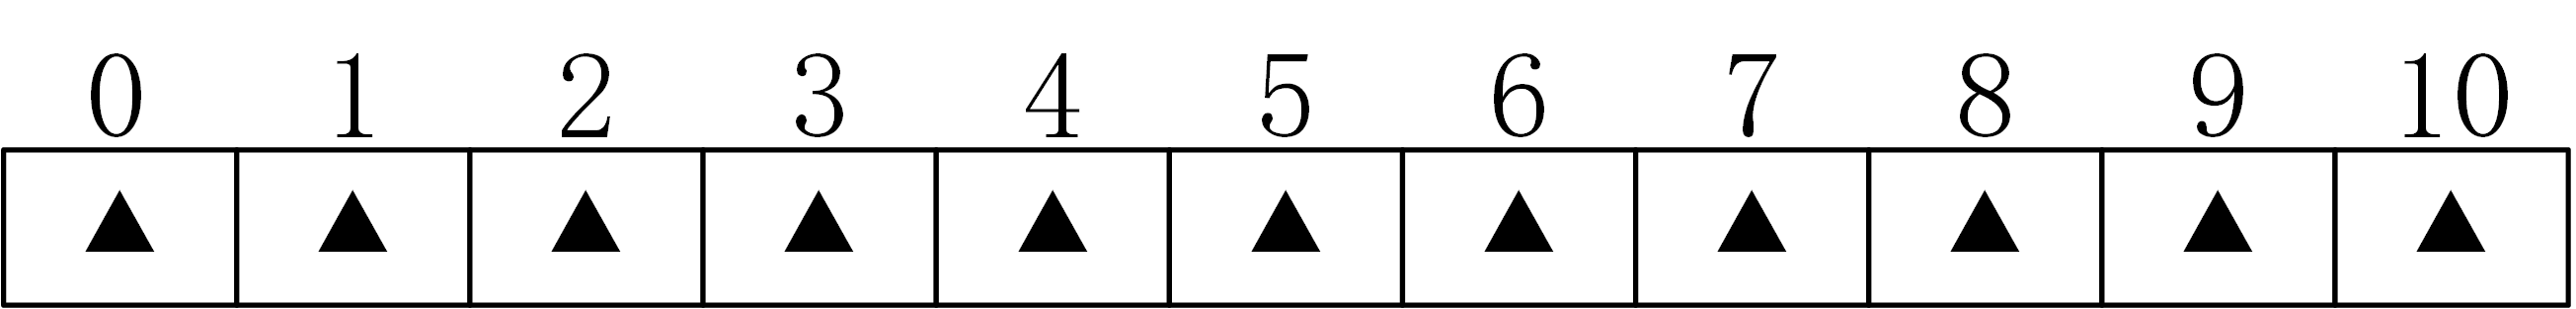
\includegraphics[width=0.9\textwidth]{array}
\end{center}
线性链表:
\vspace{-2mm}
\begin{center}
  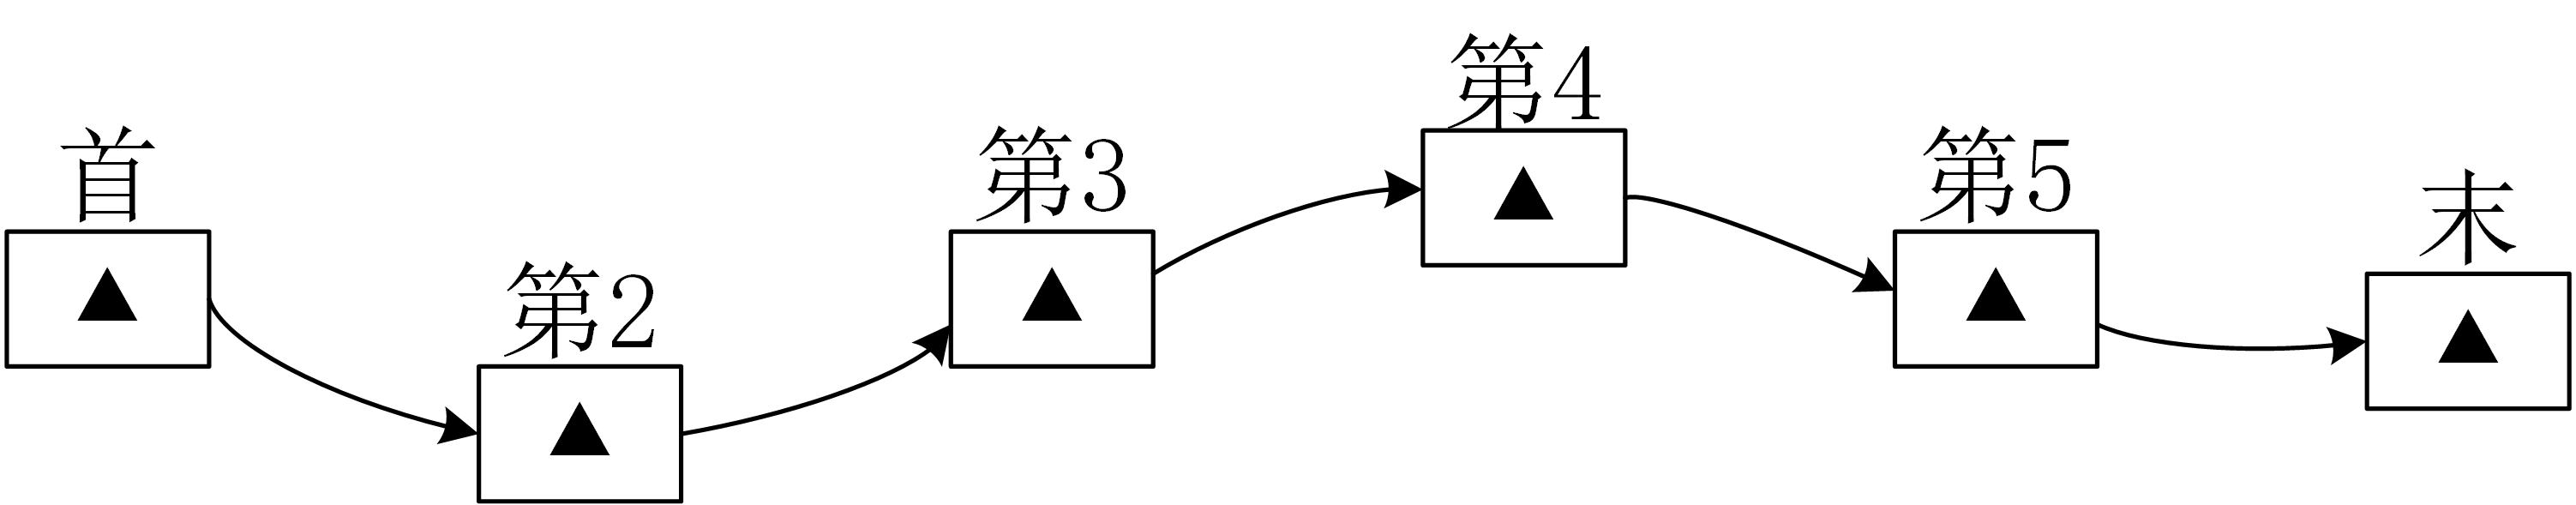
\includegraphics[width=0.9\textwidth]{linked_list}
\end{center}
链栈:
\vspace{-4mm}
\begin{center}
  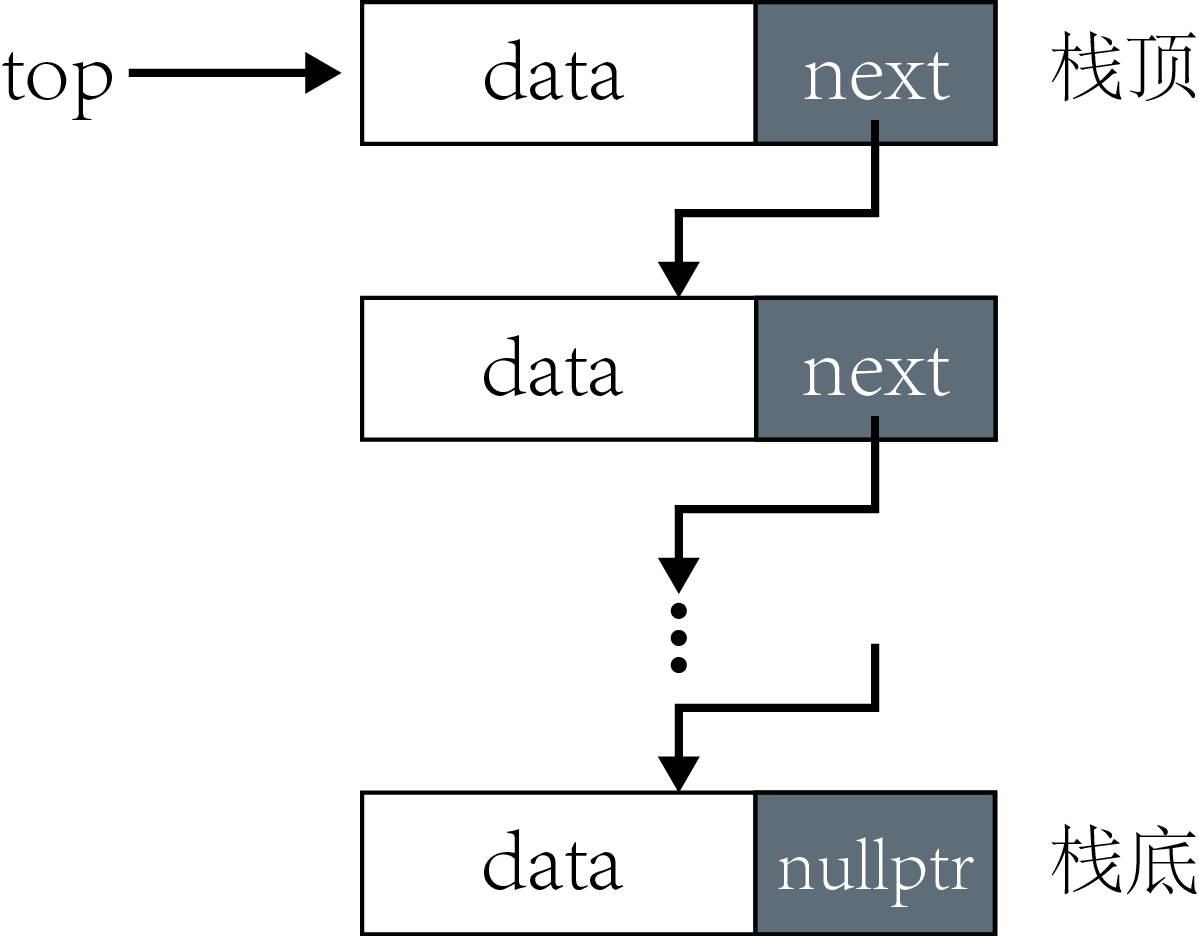
\includegraphics[width=0.4\textwidth]{stack}
\end{center}

\column{0.48\textwidth}
\begin{block}<2->{非线性结构}
一个结点可能有多个后继多个前驱
\end{block}
\uncover<2->{树:
\begin{center}
  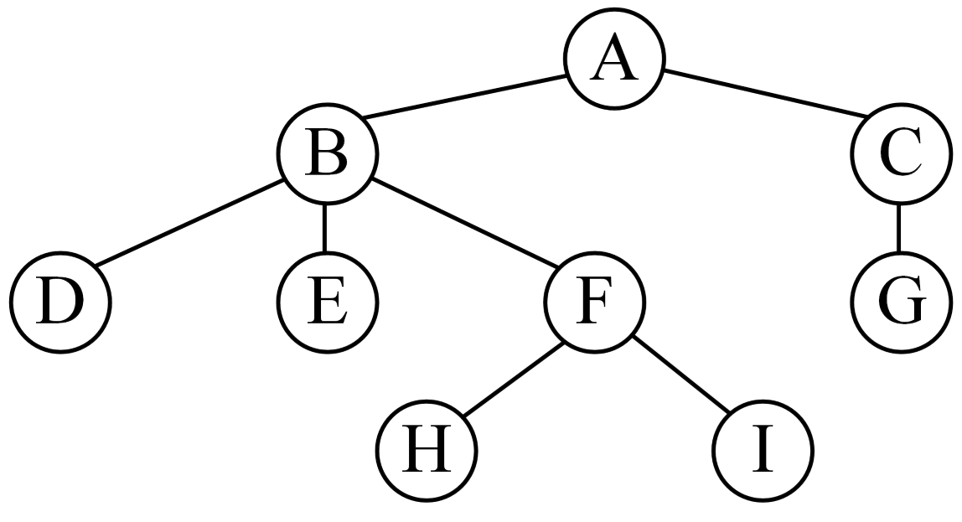
\includegraphics[width=0.55\textwidth]{tree}
\end{center}
图:
\begin{center}
  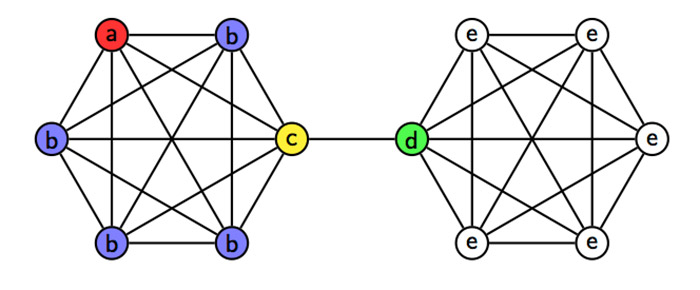
\includegraphics[width=0.9\textwidth]{graph}
\end{center}}

\end{columns}

\end{frame}

%-----------------

\begin{frame}[fragile]{8.5~二叉树}

\vspace{-4mm}

\begin{columns}

\column{0.48\textwidth}
\begin{block}{树}
\begin{center}
  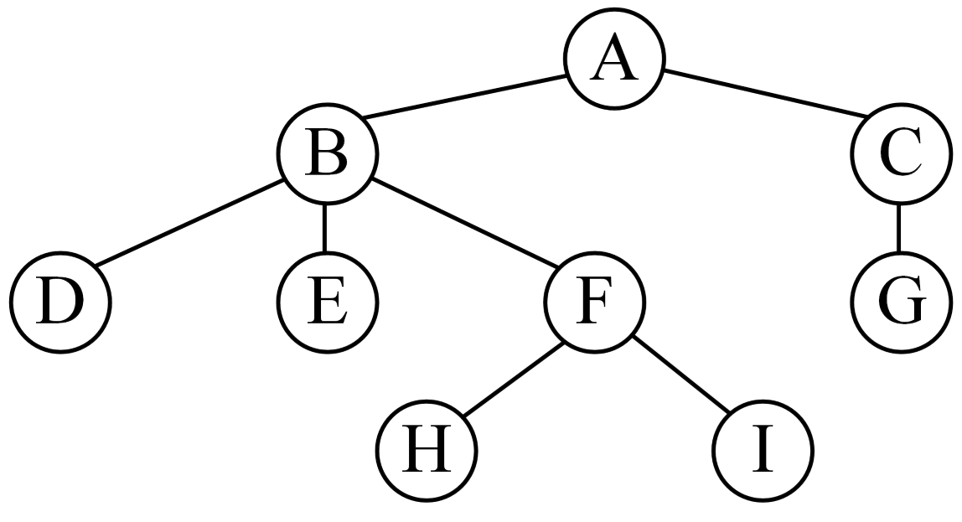
\includegraphics[width=0.8\textwidth]{tree}
\end{center}
\end{block}

\column{0.48\textwidth}
\begin{block}<2->{根结点}
一棵非空树有且仅有一个根结点
\end{block}
\vspace{-2mm}
\begin{block}<3->{子树}
除了根结点外,每个集合互不相交的结点集称为根的子树
\end{block}
\vspace{-2mm}
\begin{block}<4->{度}
每个结点的子树的数量为该结点的度
\end{block}
\vspace{-2mm}
\begin{block}<5->{叶子结点}
度为0的结点称为叶子结点
\end{block}
\vspace{-2mm}
\begin{block}<6->{子结点}
每个结点的子树的根结点称为该结点的子结点
\end{block}

\end{columns}

\end{frame}

%-----------------

%++++++++++++++++++++++++++++++++++++++++++++++
\subsection{二叉树的概念和表示}
%++++++++++++++++++++++++++++++++++++++++++++++

%-----------------

\begin{frame}[fragile]{8.5.1~二叉树的概念和表示}

\begin{block}{二叉树}
\begin{center}
  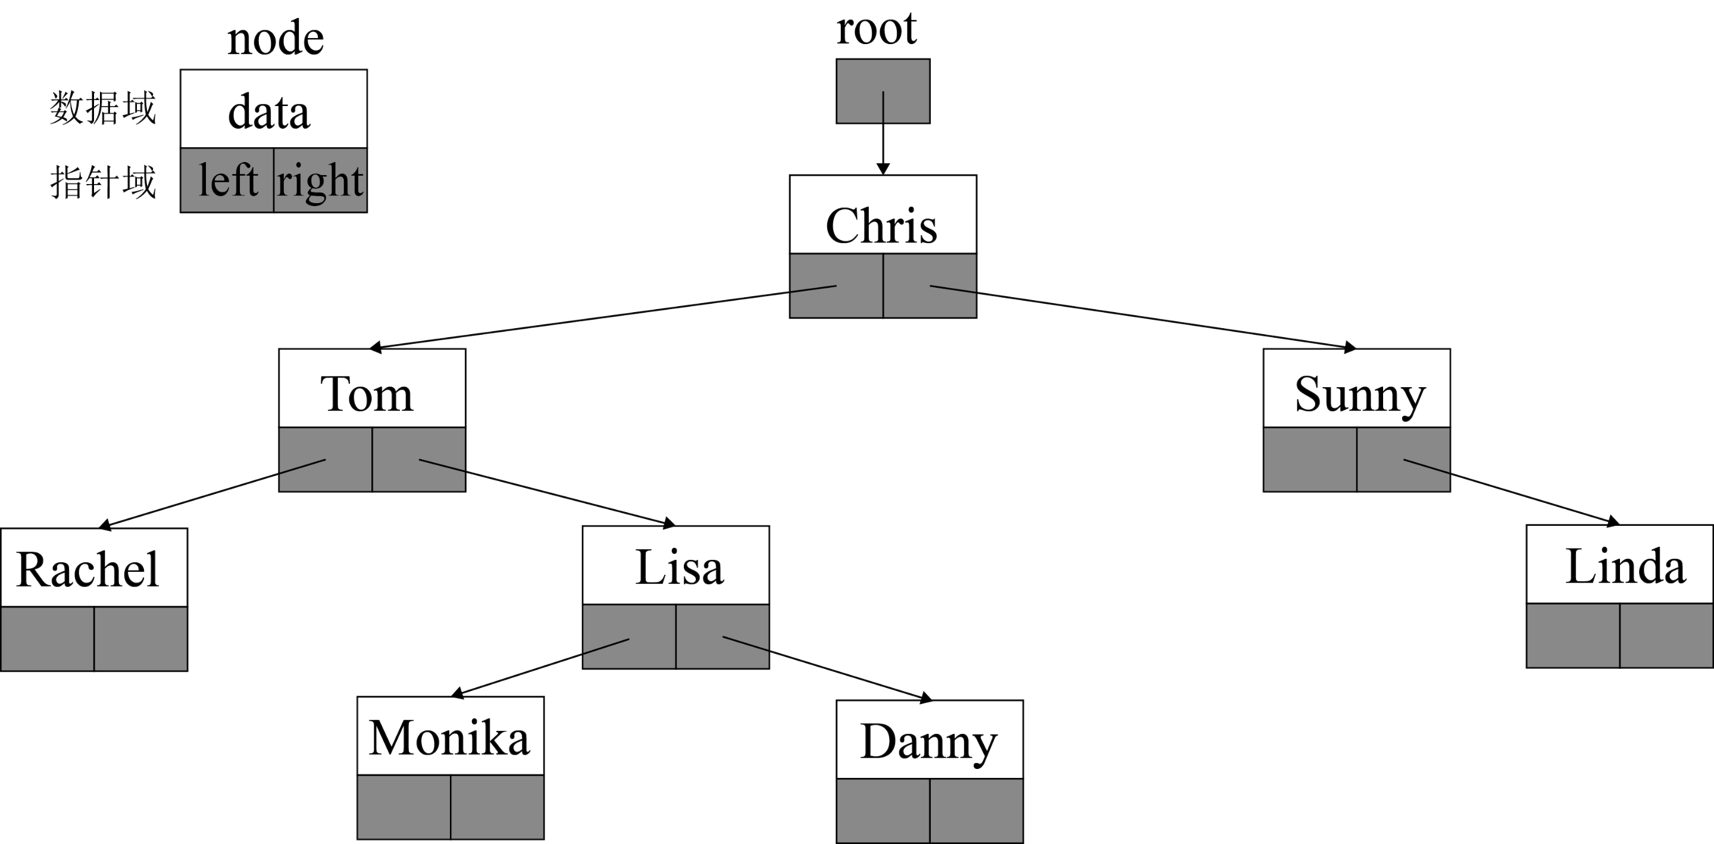
\includegraphics[width=0.6\textwidth]{binary_tree}
\end{center}
\end{block}

\begin{block}<2->{}
每个结点的\alert{子结点数目不超过2}
\end{block}

\begin{block}<3->{}
每个结点的两个子树也称为该结点的左子树和右子树
\end{block}

\end{frame}

%-----------------

\begin{frame}[fragile]{8.5.1~二叉树的概念和表示}

二叉树结点的定义如下:

\vspace{-4mm}

\begin{columns}[t]

\column{0.65\textwidth}
\begin{blueblock}{二叉树结点类模板\texttt{Node}定义}
\vspace{-2.5mm}\begin{lstlisting}[moreemph={Node,T}]
template<typename T>
class Node {
private:
    T m_data;
    Node *m_left = nullptr, *m_right = nullptr;
public:
    Node(const T &data):m_data(data){}
    T& data() { return m_data; }
    const T& data() const{ return m_data; }
    Node* left() { return m_left; }
    Node* right() { return m_right; }
};
\end{lstlisting}\vspace{-2.5mm}
\end{blueblock}

\column{0.3\textwidth}
\begin{yellowblock}{说明}
$\bullet$~数据成员\texttt{m\_data}表示一个结点的数据域\\
$\bullet$~成员指针\texttt{m\_left}和\texttt{m\_right}分别为结点的左子树和右子树的根结点的指针
\end{yellowblock}

\end{columns}

\end{frame}

%-----------------

\begin{frame}[fragile]{8.5.1~二叉树的概念和表示}

\begin{block}{二叉搜索树}
\begin{center}
  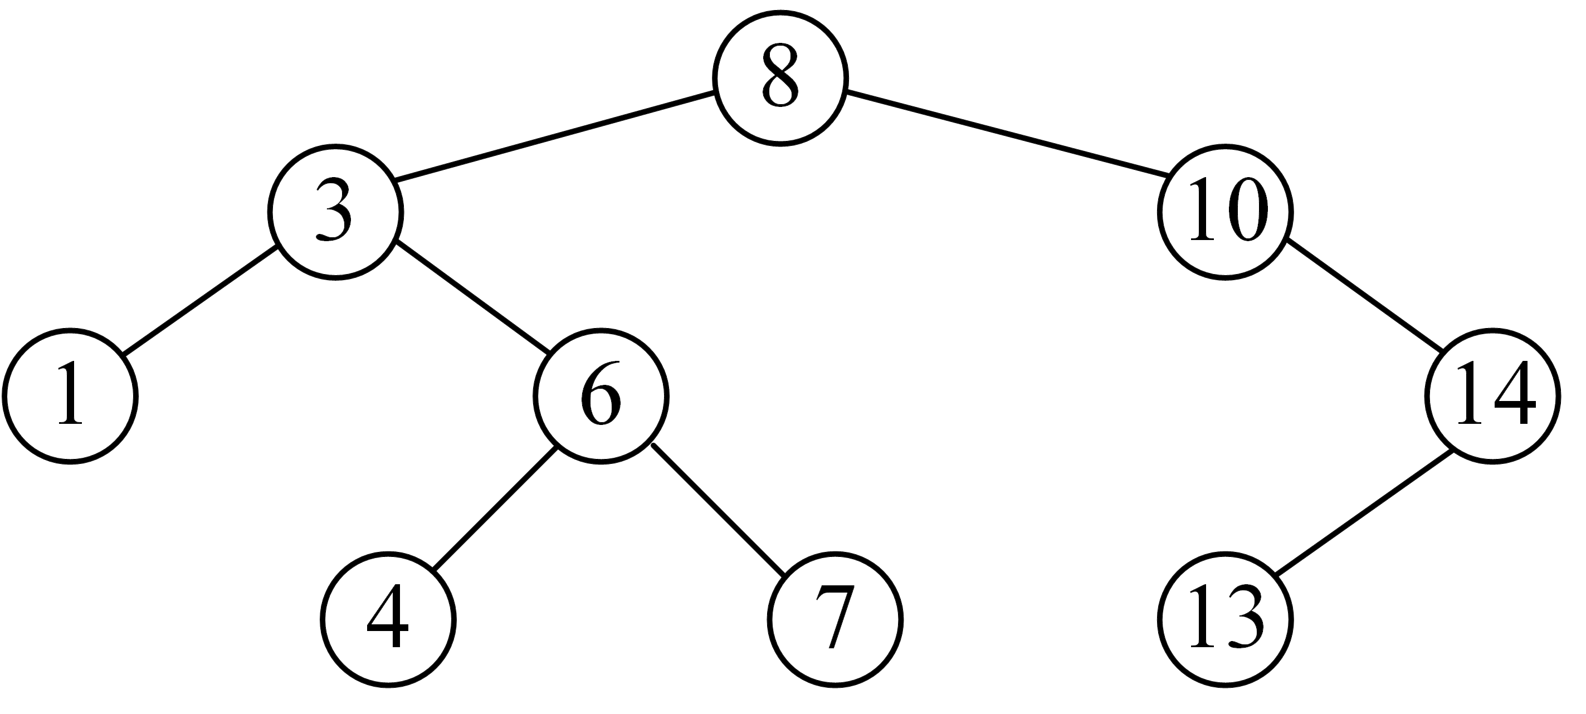
\includegraphics[width=0.45\textwidth]{binary_search_tree}
\end{center}
\end{block}

\begin{block}<2->{}
任意一个结点的\alert{左子树}中的数据值都\alert{小于}该结点的数据值,\alert{右子树}的数据值都\alert{大于或等于}该结点的数据值
\end{block}

\end{frame}

%-----------------

\begin{frame}[fragile]{8.5.1~二叉树的概念和表示}

定义一个二叉搜索树类,包含插入结点、遍历、查找、销毁子树等操作:

\vspace{-4mm}

\begin{columns}[t]

\column{0.68\textwidth}
\begin{blueblock}{\texttt{BinaryTree}类模板定义}
\vspace{-2.5mm}\begin{lstlisting}[moreemph={BinaryTree,Node,T}]
template<typename T>
class BinaryTree{
public:
    ~BinaryTree() { destroy(m_root); }
    Node<T>* root() const { return m_root; }
    Node<T>* insert(const T &value){
        return insert_(m_root, value);//返回新建结点指针
    }
    Node<T>* search(const T &value)const{
        return search_(m_root, value);
    }
    void inOrder(Node<T> *p,void (*visit)(Node<T>&));
private:
    Node<T>* search_(Node<T> *p, const T &value) const;
    Node<T>* insert_(Node<T> * &p, const T &value);
    void destroy(Node<T> *p);
private:
    Node<T> *m_root = nullptr;
};
\end{lstlisting}\vspace{-2.5mm}
\end{blueblock}

\column{0.27\textwidth}
\begin{yellowblock}{说明}
$\bullet$~\texttt{insert}和析构函数都分别调用私有成员函数\texttt{insert\_}和\texttt{destory},分别\alert{递归}进行插入和销毁子树操作\\
$\bullet$~\texttt{inorder}函数执行\alert{中序遍历}操作,其第二个参数为遍历时对元素进行操作的函数\\
$\bullet$~\texttt{search}函数调用\texttt{search\_},从\alert{根结点}开始进行\alert{二分搜索}
\end{yellowblock}

\end{columns}

\end{frame}

%-----------------

%++++++++++++++++++++++++++++++++++++++++++++++
\subsection{创建二叉搜索树}
%++++++++++++++++++++++++++++++++++++++++++++++

%-----------------

\begin{frame}[fragile]{8.5.2~创建二叉搜索树}

通过逐个插入元素来创建二叉搜索树:

\vspace{-4mm}

\begin{columns}[t]

\column{0.65\textwidth}
\begin{blueblock}{创建二叉搜索树}
\begin{lstlisting}[moreemph={BinaryTree,Node}]
int keys[] = { 8,3,10,1,6,14,4,7,13 };
BinaryTree<int> bstree;
    for (auto i:keys)
        if (Node<int> *n=bstree.insert(i) )
            cout << n->data() << " ";
\end{lstlisting}
\end{blueblock}

\uncover<2->{\texttt{\alert<3>{8},\alert<4>{3},\alert<5>{10},\alert<6>{1},\alert<7>{6},\alert<8>{14},\alert<9>{4},\alert<10>{7},\alert<11>{13}}}

\only<3>{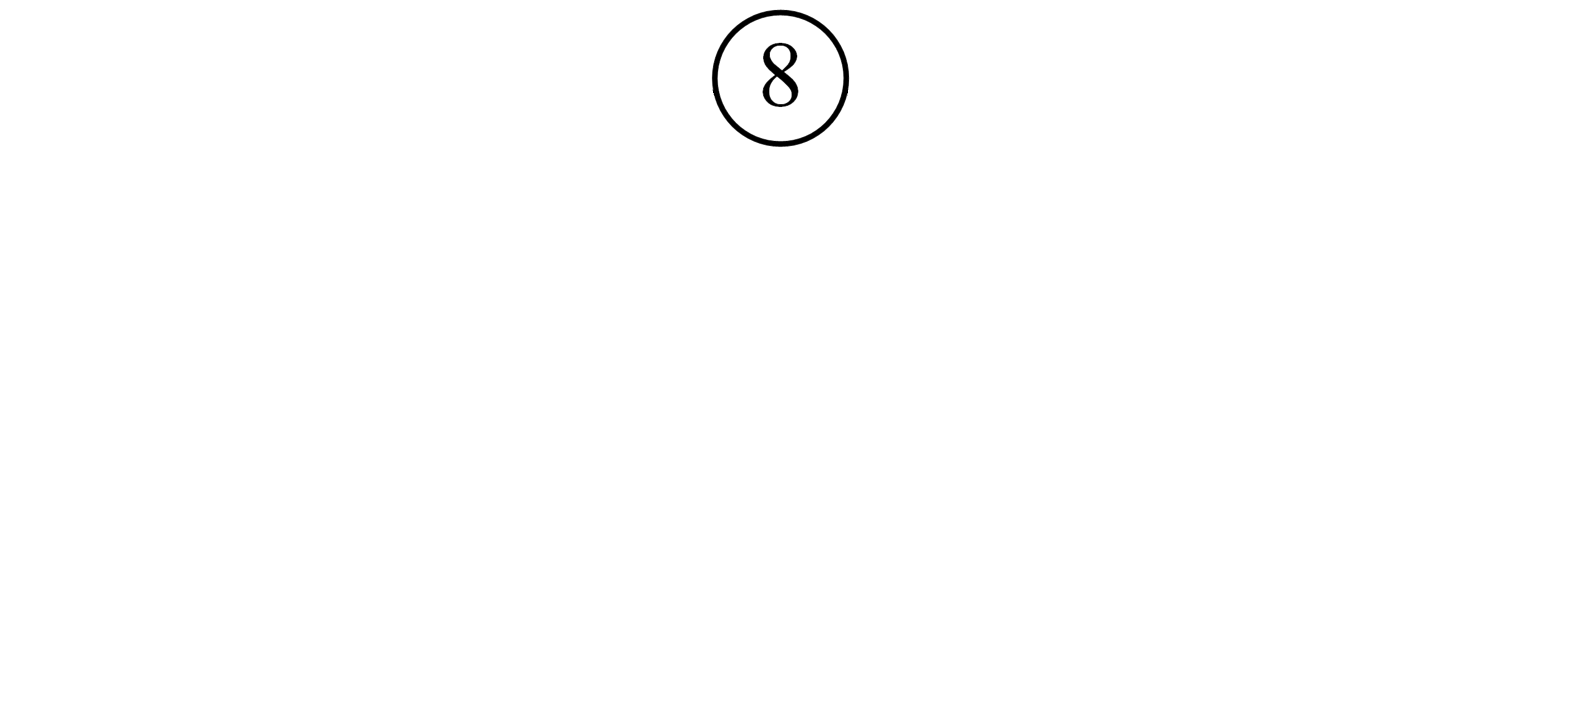
\includegraphics[width=0.7\textwidth]{create_binary_tree_1}}
\only<4>{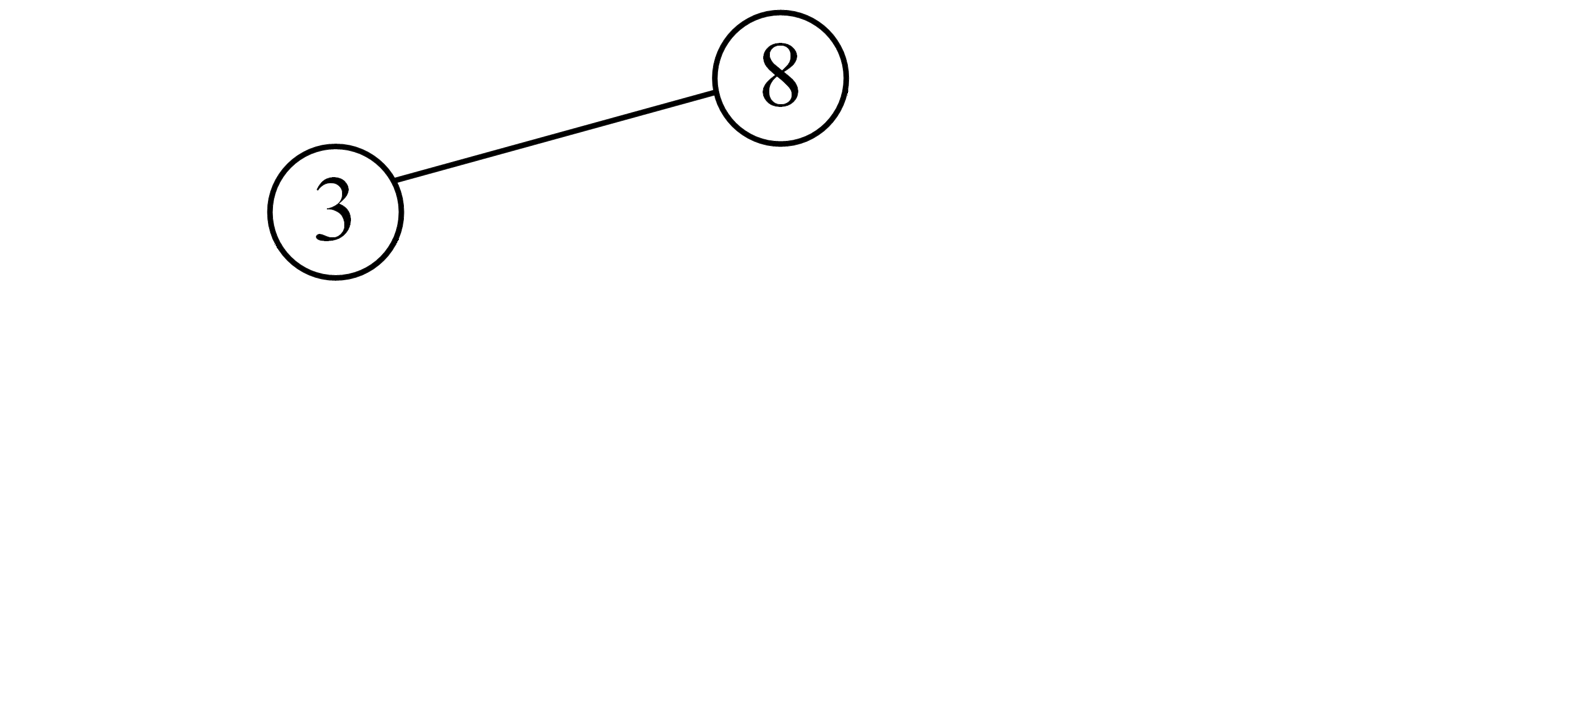
\includegraphics[width=0.7\textwidth]{create_binary_tree_2}}
\only<5>{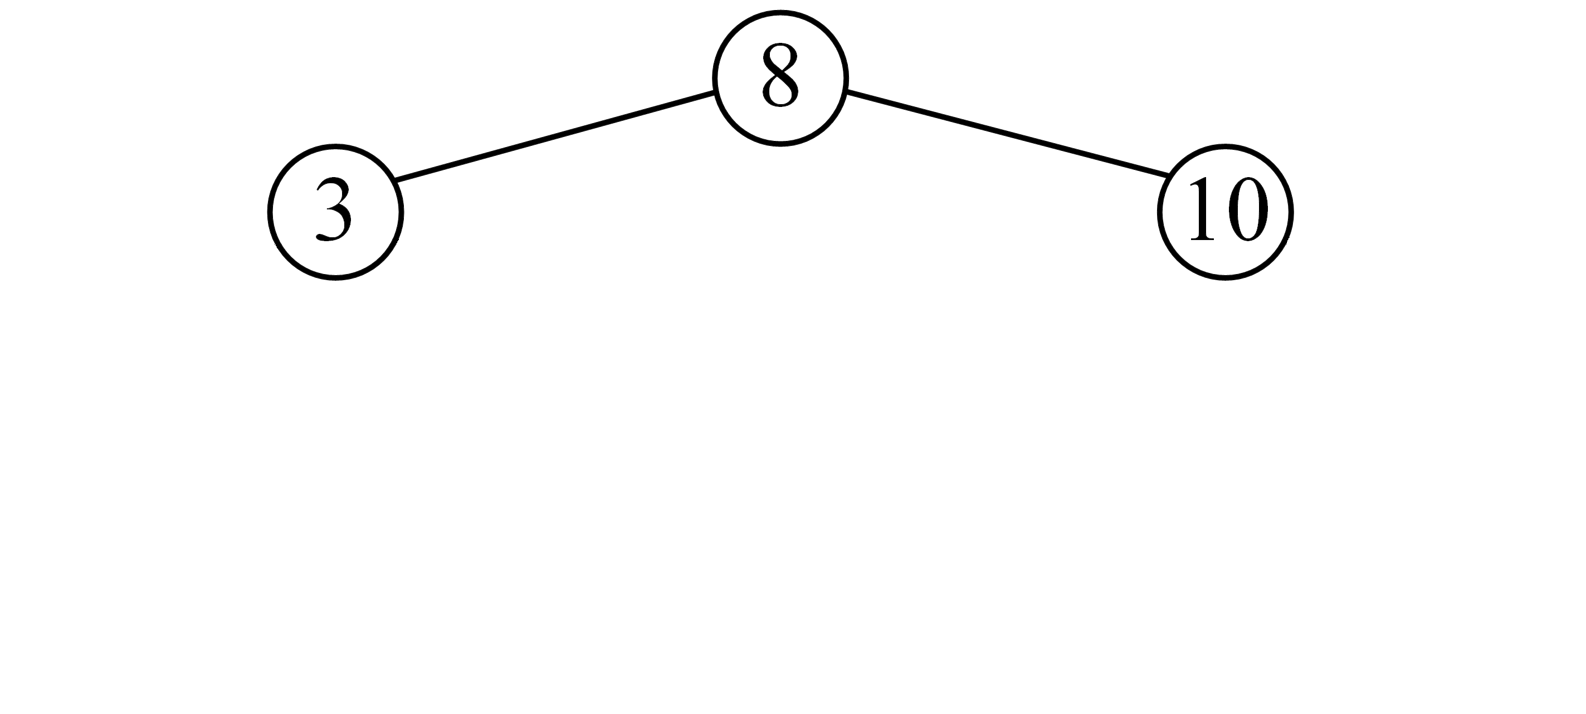
\includegraphics[width=0.7\textwidth]{create_binary_tree_3}}
\only<6>{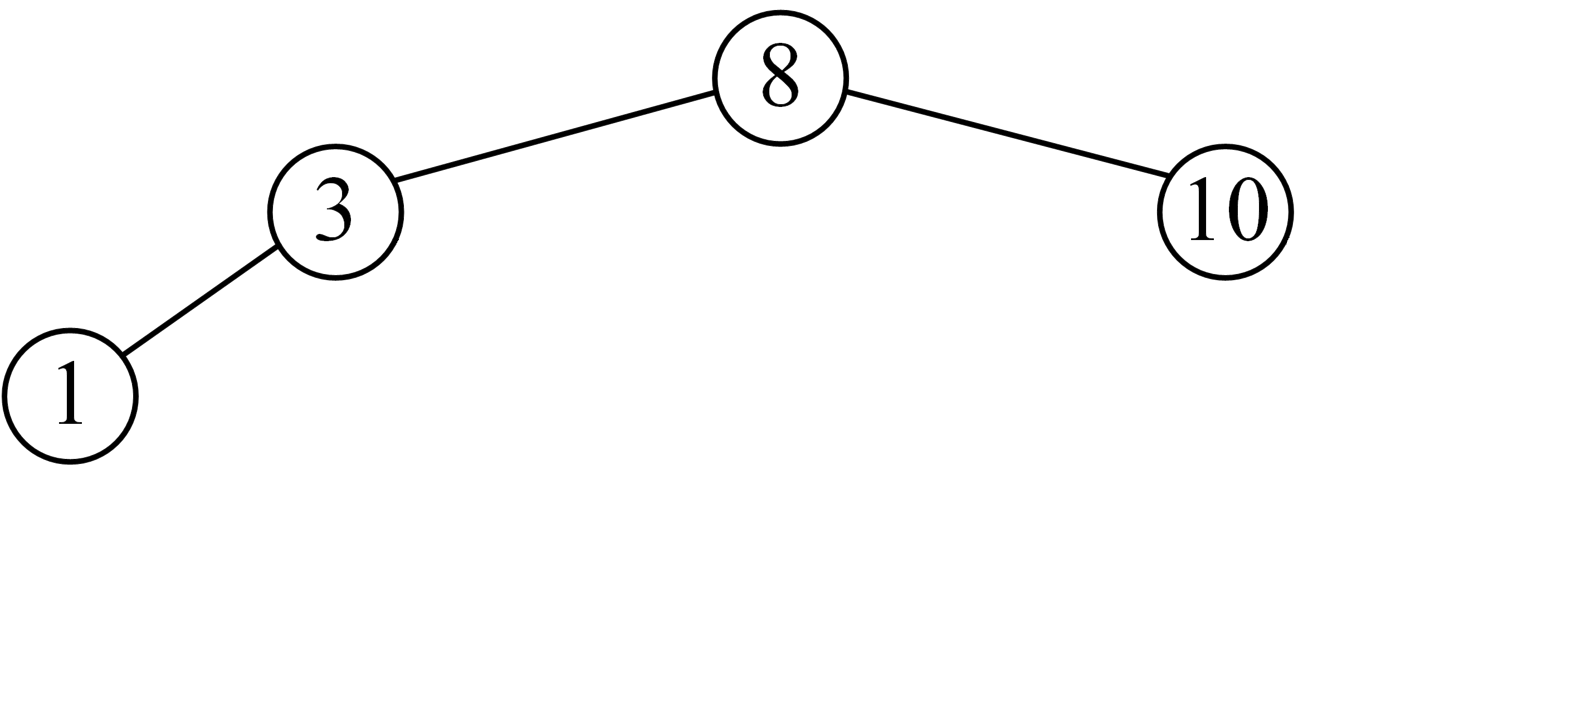
\includegraphics[width=0.7\textwidth]{create_binary_tree_4}}
\only<7>{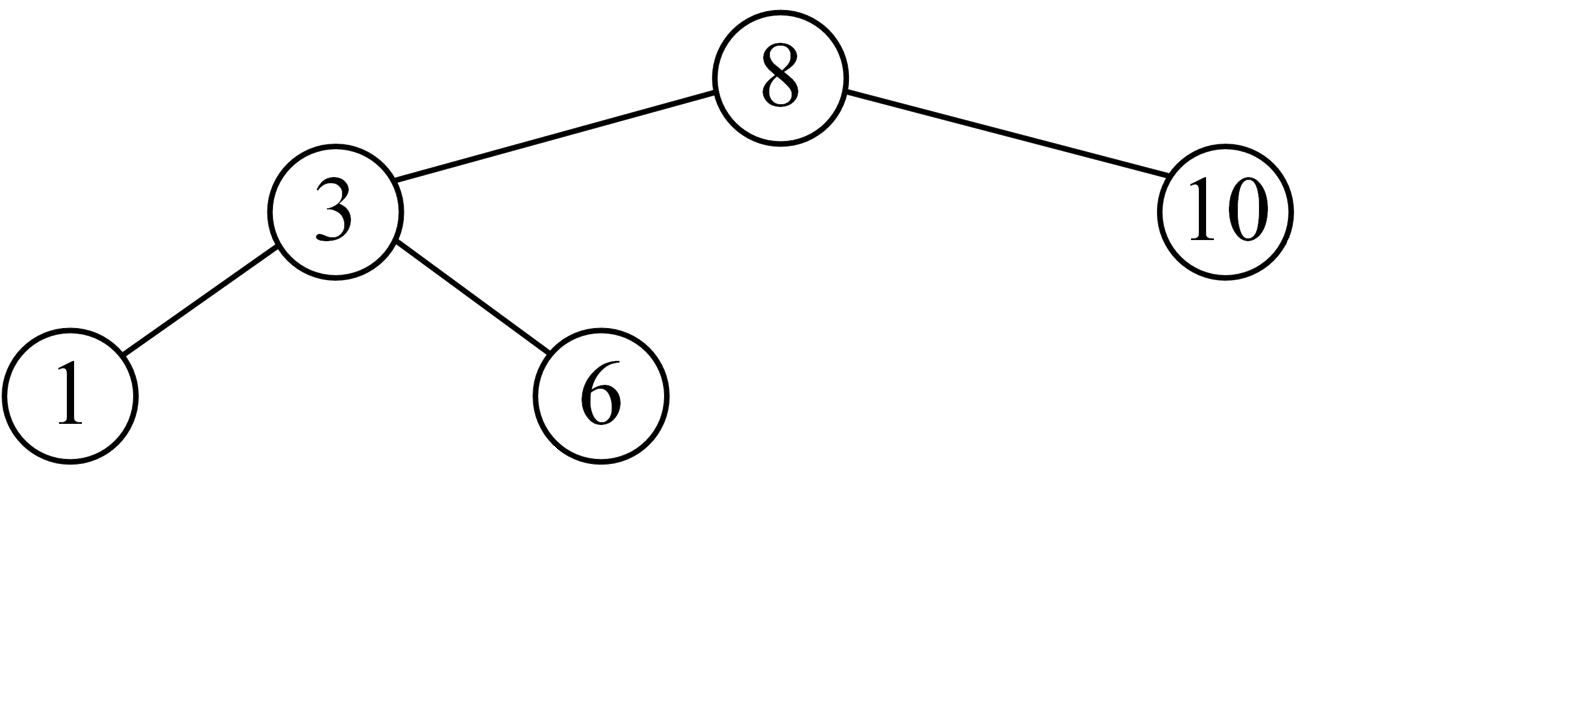
\includegraphics[width=0.7\textwidth]{create_binary_tree_5}}
\only<8>{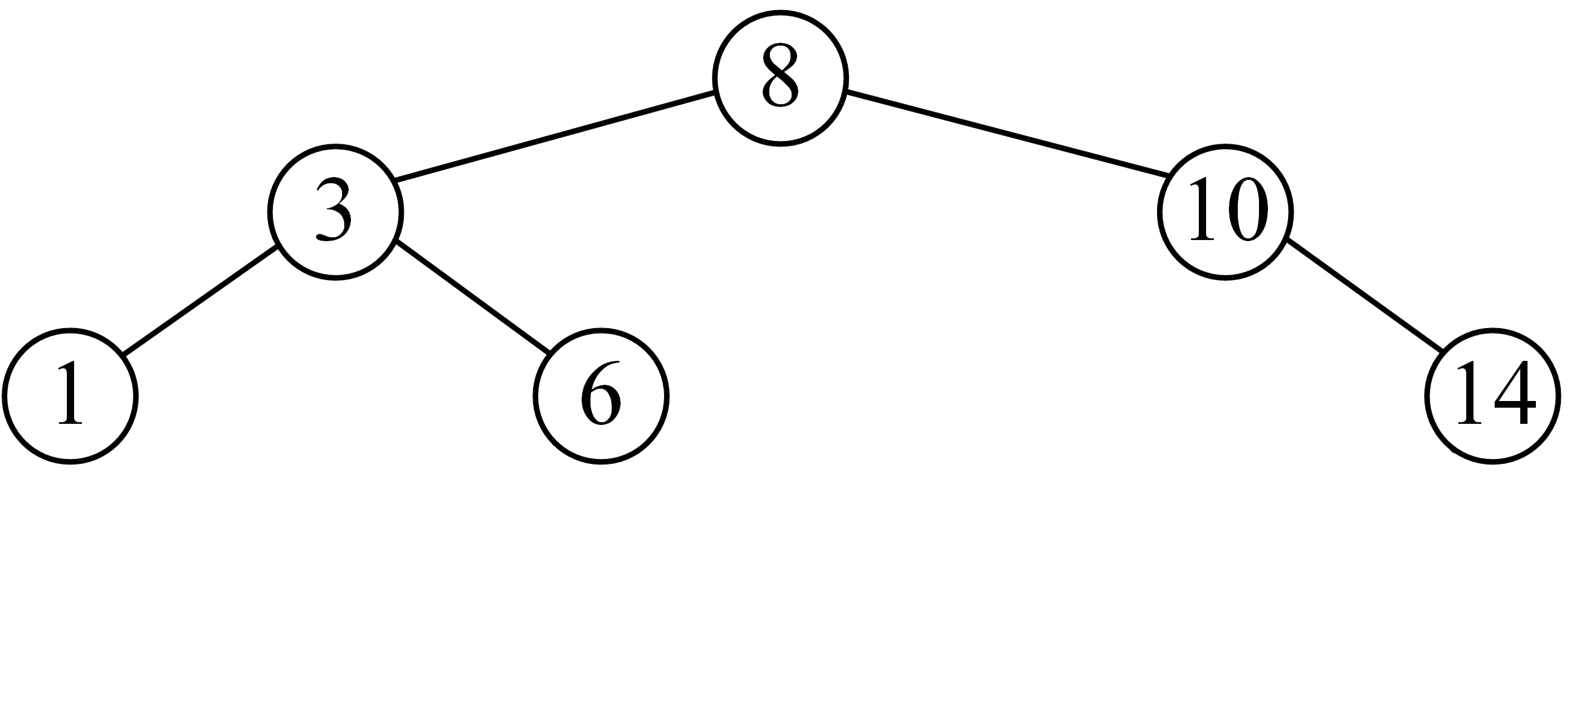
\includegraphics[width=0.7\textwidth]{create_binary_tree_6}}
\only<9>{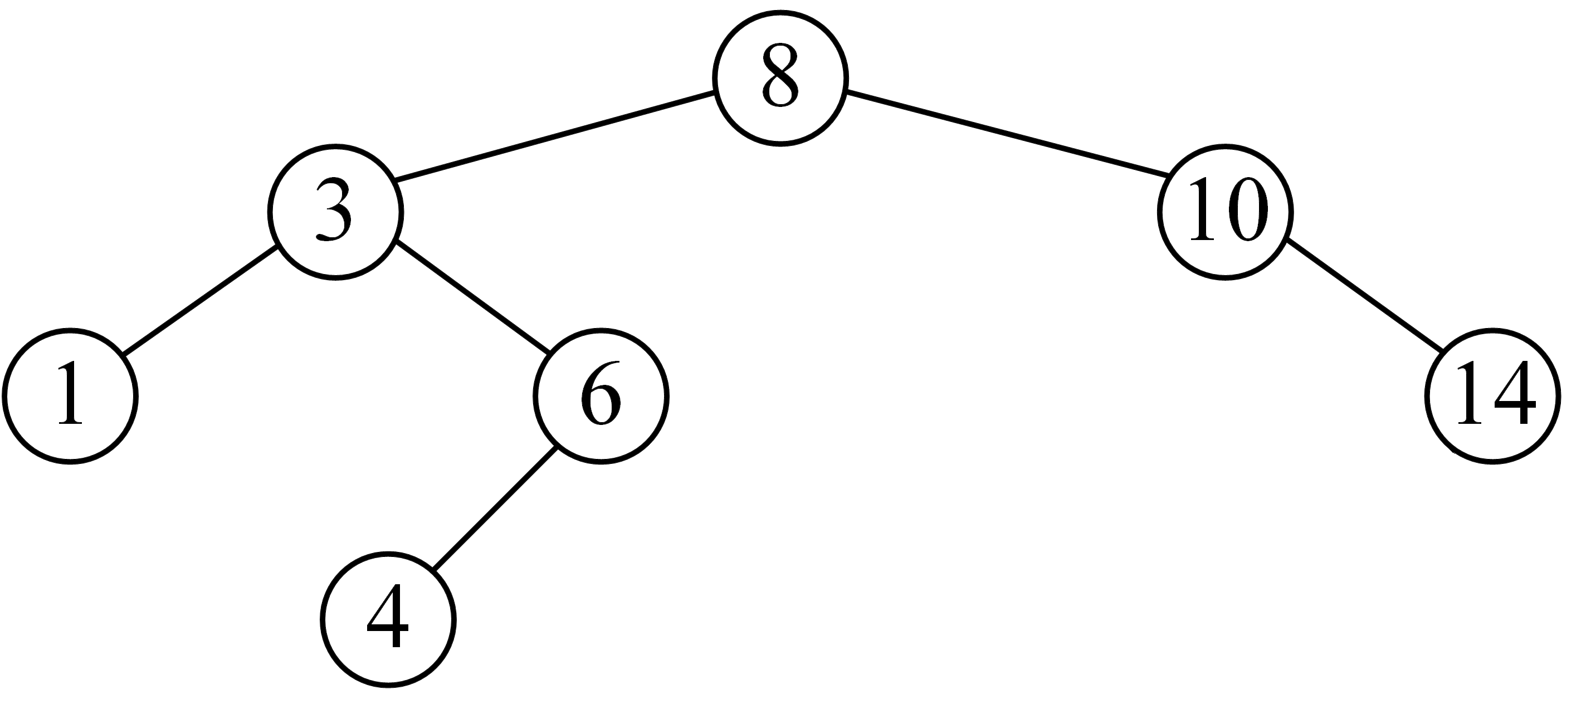
\includegraphics[width=0.7\textwidth]{create_binary_tree_7}}
\only<10>{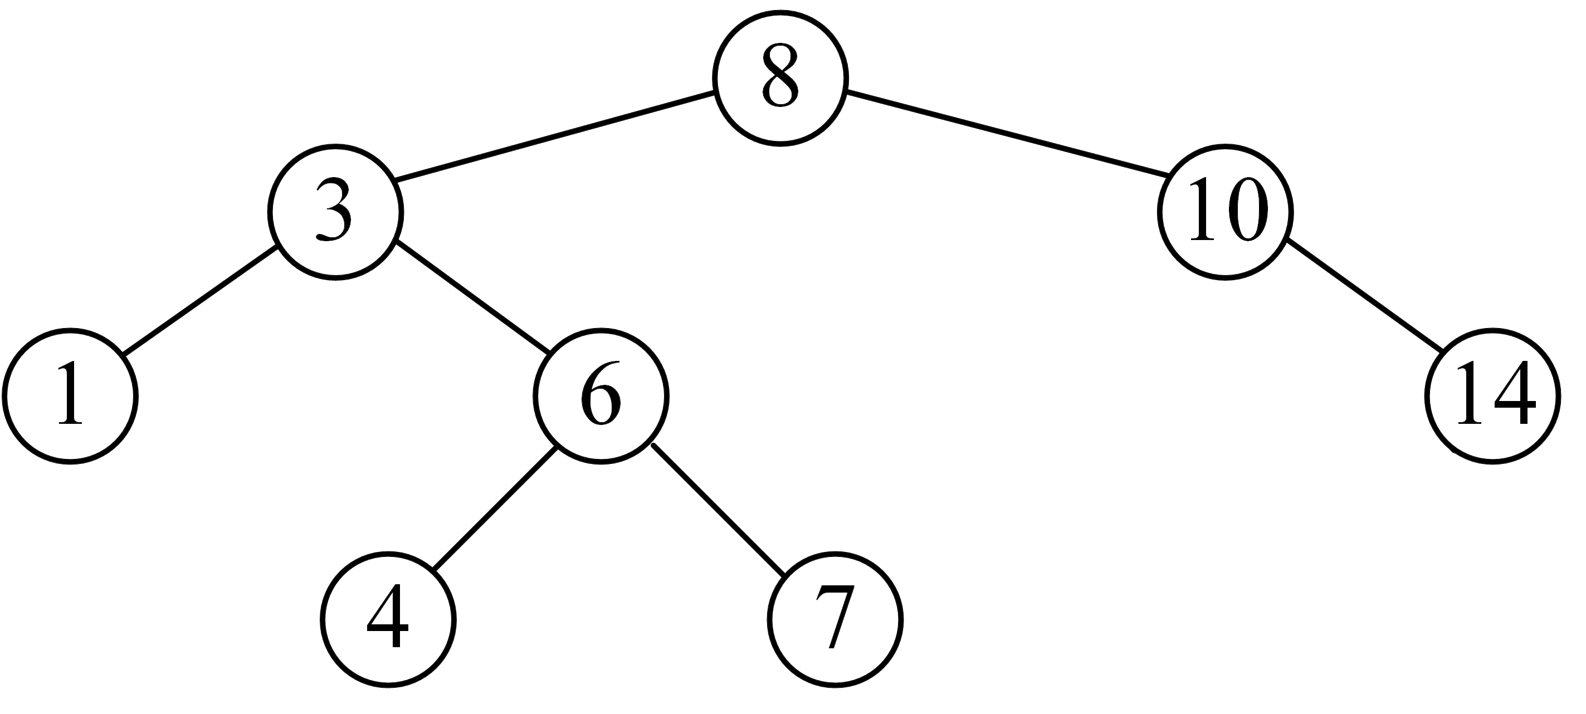
\includegraphics[width=0.7\textwidth]{create_binary_tree_8}}
\only<11->{\includegraphics[width=0.7\textwidth]{create_binary_tree_9}}

\column{0.3\textwidth}
\begin{yellowblock}{说明}
插入新结点成功则返回结点指针,然后打印数据
\end{yellowblock} \vspace{-2mm}
\begin{yellowblock}<2->{说明}
从根结点开始,若待插入结点小于根结点,则在左子树上继续查找插入位置;否则在右子树中查找
\end{yellowblock}\vspace{-2mm}
\begin{greenblock}<12->{问题}
如果改变插入顺序,如将\texttt{1}调到第一个插入,树的结构会有多大变化?
\end{greenblock}

\end{columns}

\end{frame}

%-----------------

\begin{frame}[fragile]{8.5.2~创建二叉搜索树}

成员函数\texttt{insert\_}的实现如下:

\vspace{-4mm}

\begin{columns}[t]

\column{0.65\textwidth}
\begin{blueblock}{创建二叉搜索树}
\begin{lstlisting}[moreemph={BinaryTree,T,Node}]
template<typename T>
Node<T> * BinaryTree<T>::insert_(Node<T>* (*@{\alert \&}@*)p, const T &value){
    if (p == nullptr)                           //找到插入位置,创建新结点
        return p = new (std::nothrow) Node<T>(value);
    else if (value < p->m_data)
        return insert_(p->m_left, value);       //在左子树中查找
    else
        return insert_(p->m_right, value);       //在右子树中查找
}
\end{lstlisting}
\end{blueblock}

\column{0.3\textwidth}
\begin{yellowblock}{说明}
如果\texttt{new}运算失败,\texttt{std::nothrow}保证返回空指针
\end{yellowblock}
\vspace{-2mm}
\begin{greenblock}<2->{问题}
第一个形参\alert{必须}为\texttt{Node}类型的\alert{指针的引用},而不是指针,为什么?
\end{greenblock}
\vspace{-2mm}
\begin{greenblock}<3->{答案}
否则创建新结点时,只有局部对象\texttt{p}被改指向新的动态内存地址,真正的实参的值还是\texttt{nullptr}
\end{greenblock}

\end{columns}

\end{frame}

%-----------------

%++++++++++++++++++++++++++++++++++++++++++++++
\subsection{遍历操作}
%++++++++++++++++++++++++++++++++++++++++++++++

%-----------------

\begin{frame}[fragile]{8.5.3~遍历操作}

\vspace{-2mm}

\begin{columns}[t]

\column{0.65\textwidth}
\begin{block}{二叉树的遍历}
\begin{itemize}
  \item 根据某种次序访问树中每个结点一次且仅一次
  \item 访问的过程中可以根据需要对结点的数据进行不同的处理操作,但\alert{不能}改变原来的结构
\end{itemize}
\end{block}
\uncover<2->{\begin{center}
\includegraphics[width=\textwidth]{binary_search_tree}
\end{center}}

\column{0.3\textwidth}
\begin{block}<2->{先序遍历}
\alert{根结点}-->左子树-->右子树\\
\texttt{\uncover<3->{8} \uncover<4->{3} \uncover<5->{1} \uncover<6->{6} \uncover<7->{4} \uncover<8->{7} \uncover<9->{10} \uncover<10->{14} \uncover<11->{13}}
\end{block}
\begin{block}<12->{中序遍历}
左子树-->\alert{根结点}-->右子树\\
\texttt{\uncover<13->{1} \uncover<14->{3} \uncover<15->{4} \uncover<16->{6} \uncover<17->{7} \uncover<18->{8} \uncover<19->{10} \uncover<20->{13} \uncover<21->{14}}\\
\alert{\uncover<22->{有序序列}}
\end{block}
\begin{block}<23->{后序遍历}
左子树-->右子树-->\alert{根结点}\\
\texttt{\uncover<24->{1} \uncover<25->{4} \uncover<26->{7} \uncover<27->{6} \uncover<28->{3} \uncover<29->{13} \uncover<30->{14} \uncover<31->{10} \uncover<32->{8}}
\end{block}

\end{columns}

\end{frame}

%-----------------

\begin{frame}[fragile]{8.5.3~遍历操作}

以中序遍历的实现为例:

\vspace{-5mm}

\begin{columns}[t]
\column{0.72\textwidth}
\begin{blueblock}{示例代码}
\vspace{-3mm}\begin{lstlisting}[moreemph={BinaryTree,Node}]
template<typename T>
void BinaryTree<T>::inOrder(Node<T> *p,void (*visit)(T&)){
    if (p != nullptr){
        inOrder(p->m_left, visit); //遍历左子树
        visit(p->m_data); //用户自定义访问函数
        inOrder(p->m_right, visit); //遍历右子树
    }
}
\end{lstlisting}\vspace{-2.5mm}
\end{blueblock}

\column{0.23\textwidth}
\begin{yellowblock}{说明}
第二个形参为一个返回值为空、包含一个\texttt{T\&}类型形参的函数指针,指向用户自定义的访问处理函数
\end{yellowblock}
\end{columns}

\uncover<2->{定义一个简单的访问函数模板:}

\vspace{-4mm}

\begin{columns}[t]
\column{0.72\textwidth}
\begin{blueblock}<2->{\texttt{visit}函数模板定义}
\vspace{-3mm}\begin{lstlisting}[moreemph={BinaryTree,T,Node}]
template<typename T> void visit(T &value) { cout << value << " "; }
\end{lstlisting}\vspace{-3mm}
\end{blueblock}

\column{0.23\textwidth}
\begin{yellowblock}<2->{说明}
打印结点的数据
\end{yellowblock}

\end{columns}

\uncover<3->{中序遍历之前创建的二叉搜索树:}

\vspace{-4mm}
\begin{columns}[t]
\column{0.72\textwidth}
\begin{blueblock}<3->{}
\vspace{-3mm}\begin{lstlisting}[moreemph={BinaryTree,T,Node}]
bstree.inOrder(bstree.root(), visit<int>);
输出结果为:1 3 4 6 7 8 10 13 14
\end{lstlisting}\vspace{-3mm}
\end{blueblock}

\column{0.23\textwidth}

\end{columns}

\end{frame}

%-----------------

%++++++++++++++++++++++++++++++++++++++++++++++
\subsection{搜索操作}
%++++++++++++++++++++++++++++++++++++++++++++++

%-----------------

\begin{frame}[fragile]{8.5.4~搜索操作}

根据二叉排序树的性质,可以采用\alert{二分法}来实现快速搜索:

\vspace{-4mm}

\begin{columns}[t]

\column{0.72\textwidth}
\begin{blueblock}{成员函数\texttt{search\_}定义}
\vspace{-3mm}\begin{lstlisting}[moreemph={BinaryTree,T,Node}]
template<typename T>
Node<T>* BinaryTree<T>::search_(Node<T> *p, const T &value)const{
    while (p != nullptr && p->m_data != value){
        if (value < p->m_data)
            p = p->m_left;
        else
            p = p->m_right;
    }
    return p;
}
\end{lstlisting}\vspace{-3mm}
\end{blueblock}

\column{0.23\textwidth}
\begin{yellowblock}{说明}
将返回第一个数据值为\texttt{value}的结点的指针
\end{yellowblock}

\end{columns}

\end{frame}

%-----------------

%++++++++++++++++++++++++++++++++++++++++++++++
\subsection{销毁操作}
%++++++++++++++++++++++++++++++++++++++++++++++

%-----------------

\begin{frame}[fragile]{8.5.5~销毁操作}

采用后序方式逐个释放每个结点的内存:

\vspace{-4mm}

\begin{columns}[t]

\column{0.72\textwidth}
\begin{blueblock}{成员函数\texttt{destroy}定义}
\vspace{-3mm}\begin{lstlisting}[moreemph={BinaryTree,T,Node}]
template<typename T>
void BinaryTree<T>::destroy(Node<T> *p){
    if (p != nullptr){
        destroy(p->m_left);//销毁左子树
        destroy(p->m_right);//销毁右子树
        delete p;//释放根结点内存
    }
}
\end{lstlisting}\vspace{-3mm}
\end{blueblock}

\column{0.23\textwidth}
\begin{yellowblock}{说明}
$\bullet$~释放给定结点及其左右子树的内存\\
$\bullet$~访问权限声明为私有,是析构函数的实现
\end{yellowblock}
\begin{redblock}<2->{注意}
若在它处执行此函数后,必须把给定结点的父结点(如有)指向此结点的指针成员置空,否则成为\alert{空悬指针}
\end{redblock}


\end{columns}

\end{frame}

%-----------------

%++++++++++++++++++++++++++++++++++++++++++++++
\subsection{拷贝控制及友元声明}
%++++++++++++++++++++++++++++++++++++++++++++++

%-----------------

\begin{frame}[fragile]{8.5.6~拷贝控制及友元声明}

类似于单链表,二叉树中的结点以及二叉树本身不允许执行默认的拷贝成员,因此将它们声明为\texttt{delete}

\vspace{-4mm}

\begin{columns}[t]

\column{0.72\textwidth}
\begin{blueblock}{\texttt{BianryTree}和\texttt{Node}类模板的拷贝控制及友元声明}\textsl{}
\vspace{-3mm}\begin{lstlisting}[moreemph={BinaryTree,T,Node}]
template<typename T> class BinaryTree;//前向声明
template<typename T>
class Node{
friend class BinaryTree<T>;
public:
    Node(const Node&) = delete;
    Node& operator=(const Node&) = delete;
    //其它成员保持不变
};
template<typename T>
class BinaryTree{
public:
    BinaryTree() = default; //使用默认的构造函数
    BinaryTree(const BinaryTree &) = delete;
    BinaryTree& operator=(const BinaryTree &) = delete;
    //其它成员保持不变
};
\end{lstlisting}\vspace{-3mm}
\end{blueblock}

\column{0.23\textwidth}
\begin{yellowblock}{说明}
同时将\texttt{BinaryTree}类模板声明为\texttt{Node}类模板的友元
\end{yellowblock}

\end{columns}

\end{frame}

%-----------------

\begin{frame}[c]{~}
\begin{center}
  \huge{本章结束}
  \begin{block}{上机作业}
 \begin{enumerate}
   \item 实验指导书:第八章
   \item 检查日期:待定
   \item 地点:与助教协商
   \item 特别说明:第三道题目二叉树的应用:哈夫曼编码
 \end{enumerate}
\end{block}
\end{center}
\end{frame}

%----------------------------------------------------------------------------------------

\end{document} 